% AER-Article.tex for AEA last revised 22 June 2011
\documentclass[No]{AEA}
%%%%%% NOTE FROM OVERLEAF: The mathtime package is no longer publicly available nor distributed. We recommend using a different font package e.g. mathptmx if you'd like to use a Times font.
% \usepackage{mathptmx}

% The mathtime package uses a Times font instead of Computer Modern.
% Uncomment the line below if you wish to use the mathtime package:
%\usepackage[cmbold]{mathtime}
% Note that miktex, by default, configures the mathtime package to use commercial fonts
% which you may not have. If you would like to use mathtime but you are seeing error
% messages about missing fonts (mtex.pfb, mtsy.pfb, or rmtmi.pfb) then please see
% the technical support document at http://www.aeaweb.org/templates/technical_support.pdf
% for instructions on fixing this problem.

% Note: you may use either harvard or natbib (but not both) to provide a wider
% variety of citation commands than latex supports natively. See below.

% Uncomment the next line to use the natbib package with bibtex 
%\usepackage{natbib}

% Uncomment the next line to use the harvard package with bibtex
%\usepackage[abbr]{harvard}

% This command determines the leading (vertical space between lines) in draft mode
% with 1.5 corresponding to "double" spacing.
\usepackage{graphicx, booktabs, rotating}
\usepackage{subcaption}
\usepackage{graphicx}
\usepackage{tabularx}
\newcommand{\tablexplain}[1]{\footnotesize{#1}}
\usepackage{comment}
\usepackage{hyperref}
\usepackage{pdflscape}
\draftSpacing{1.5}
\usepackage{natbib}
\newcommand{\citeg}[1]{\citep[e.g.,][]{#1}}
\usepackage{amsmath}
\usepackage{amssymb}
\usepackage{chronology}
\usepackage{epigraph}
\usepackage[nolists]{endfloat}%\newlength{\epigraphwidth}
\setlength{\epigraphwidth}{.5\textwidth}
%\newlength{\epigraphrule}
\setlength{\epigraphrule}{0pt}
\usepackage{subcaption}
%\DeclareMathOperator{\logit}{logit}
\usepackage[letterpaper, left=   1.5 in, right=  1.5 in, top= 1.5 in, bottom= 1.5in]{geometry}
% AEA.cls is a standalone class (not built on article/report/book), so it never defines the
% \if@titlepage boolean that the titling package's internals expect from the enclosing class.
% Define it (matching article.cls's own default) before loading titling, so titling.sty's
% internal \if@titlepage checks work instead of erroring out as an undefined control sequence.
\makeatletter
\newif\if@titlepage
\@titlepagefalse
\makeatother
\usepackage{titling}

%\begin{titlingpage}
\title{Decentralized Crypto Governance? \\ Transparency and Concentration in Ethereum Decision-Making}
\shortTitle{Decentralized Crypto Governance?}
\author{Cesare Fracassi, Moazzam Khoja, and Fabian Sch\"{a}r \thanks{Fracassi: University of Texas at Austin. Khoja: University of Texas at San Antonio. Sch\"{a}r: University of Basel. Data and code to replicate the results can be found at \url{https://github.com/Fintech-Research-Lab/Ethereum_Governance_Project}. We thank Ethan Abraham, Shantikiran Chanal, Haoxiang Yi, and Matthias Nadler for their invaluable contributions as research assistants, as well as Katrin Schuler, Dario Thürkauf, Vikramaditya Khanna, and the seminar participants and discussants at the Western Finance Association, University of Texas at Austin, Texas Tech University, New York University, the Swiss National Bank, the University of Zürich, and DAWO24 for their suggestions.}}
\date{\today}
\pubMonth{September}
\pubYear{2026}
\pubVolume{Vol}
\pubIssue{Issue}
\JEL{}
\Keywords{}


 
%%%%%%%%%%%%%%%%%%%%%%%%%%%%%%%%%%%%%%%%%%%%%%%%%%%%%%%%%%%%%%%%
%%%%%%%%%%%%%%%%%%%%%%%%%%%%%%%%%%%%%%%%%%%%%%%%%%%%%%%%%%%%%%%%
%%%%%%%%%%%%%%%%%%%%%%%%%%%%%%%%%%%%%%%%%%%%%%%%%%%%%%%%%%%%%%%%

\begin{document}

 \maketitle 

\begin{center}
    \textbf{Abstract}\\
\end{center}

Decentralized crypto decision making combines an open-source community with a liquid financial asset, a governance structure with no direct analog in traditional firms. This paper uses Ethereum to examine three corporate governance concerns: price-relevant information, contributor incentives, and effective control. We assemble a dataset covering the pipeline from proposal to adoption, linking participants to employment histories. We show that governance milestones affect the value of Ether. Ether experiences a 13\% run-up over the 25 trading days preceding Core EIP approval relative to Bitcoin, demonstrating that governance decisions contain economically relevant information. We then study labor-market returns to open-source contributions: EIP authors experience a 6\% increase in employment seniority and a 9\% increase in estimated compensation following proposal authorship. These effects are particularly pronounced among junior contributors, suggesting labor-market returns incentivize participation and partially substitute for traditional contractual incentives. Finally, we show that while governance discussion is broad based, effective control is substantially concentrated : ten individuals account for 62\% of implemented Core and Networking EIPs, while client development is highly concentrated among a small number of contributors. Governance control also extends beyond the formal process through dependencies on stablecoin issuers and oracle providers. Together, our findings show that Ethereum governance is broadly participatory and transparent, while information, incentives, and control remain concentrated at different stages.


 %\end{titlingpage}

\pagenumbering{gobble}

%%%%%%%%%%%%%%%%%%%%%%%%%%%%%%%%%%%%%%%%%%%%%%%%%%%%%%%%%%%%%%%%
%%%%%%%%%%%%%%%%%%%%%%%%%%%%%%%%%%%%%%%%%%%%%%%%%%%%%%%%%%%%%%%%
%%%%%%%%%%%%%%%%%%%%%%%%%%%%%%%%%%%%%%%%%%%%%%%%%%%%%%%%%%%%%%%%

\clearpage

\begin{titlingpage}


\emptythanks
\author{}

\maketitle

\begin{center}
    \textbf{Abstract}\\
\end{center}

Decentralized crypto decision making combines an open-source community with a liquid financial asset, a governance structure with no direct analog in traditional firms. This paper uses Ethereum to examine three corporate governance concerns: price-relevant information, contributor incentives, and effective control. We assemble a dataset covering the pipeline from proposal to adoption, linking participants to employment histories. We show that governance milestones affect the value of Ether. Ether experiences a 13\% run-up over the 25 trading days preceding Core EIP approval relative to Bitcoin, demonstrating that governance decisions contain economically relevant information. We then study labor-market returns to open-source contributions: EIP authors experience a 6\% increase in employment seniority and a 9\% increase in estimated compensation following proposal authorship. These effects are particularly pronounced among junior contributors, suggesting labor-market returns incentivize participation and partially substitute for traditional contractual incentives. Finally, we show that while governance discussion is broad based, effective control is substantially concentrated : Ten individuals account for 62\% of implemented Core and Networking EIPs, while client development is highly concentrated among a small number of contributors. Governance control also extends beyond the formal process through dependencies on stablecoin issuers and oracle providers. Together, our findings show that Ethereum governance is broadly participatory and transparent, while information, incentives, and control remain concentrated at different stages.



%%%%%%%%%%%%%%%%%%%%%%%%%%%%%%%%%%%%%%%%%%%%%%%%%%%%%%%%%%%%%%%%
%%%%%%%%%%%%%%%%%%%%%%%%%%%%%%%%%%%%%%%%%%%%%%%%%%%%%%%%%%%%%%%%
\clearpage
 \end{titlingpage}
\newgeometry{letterpaper, left=   1 in, right=  1 in, top=    1.5 in, bottom= 1.5in}

\pagenumbering{arabic}
\setcounter{page}{1}




\epigraph{``We reject: kings, presidents, and voting. We believe in: rough consensus and running code.''}{David Clark, \textit{IETF, 1992}}

Modern corporate governance has organized itself around three enduring questions: how to align the incentives of those who manage a project with those who hold residual claims on it, how to constrain the use of private information, and how to allocate liability and control. Each question presupposes a familiar institutional setting: a firm with employees, a board, and shareholders whose claims are mediated through securities markets. Open-source communities (OSCs) such as Linux or the Internet Engineering Task Force have long operated outside this setting, relying on volunteer contributions, informal hierarchies, and rough-consensus decision-making. Because their output was a public good with no directly tradable claim, classical governance concerns translated only loosely to these communities.

Cryptocurrencies have brought OSCs back within the reach of classical governance concerns. Each pairs an OSC governance structure with a tradable token whose value responds in real time to governance outcomes, in a market whose aggregate valuation has at times exceeded three trillion dollars. The pairing reintroduces, in new form, every classical governance concern: contributors' incentives need not align with those of token holders; contributors may possess price-relevant information; and the locus of effective control over the protocol determines whether the associated token is best characterized as a security, a commodity, or something else. This paper uses Ethereum as an empirical laboratory to examine what the three classical pillars of corporate governance look like when the firm is replaced by an OSC and the share by a token. We find that governance milestones move prices, that labor-market returns partially substitute for contractual incentives, especially for junior roles, and that effective control is concentrated at the margins of authorship and implementation despite broad participation in discussion.

Each governance pillar takes on a distinctive character in this setting. In a conventional firm, insider trading rules target a well-defined class of employees with fiduciary duties and identifiable information advantages; in a permissionless OSC, the boundary between insider and outsider is blurred, participation is voluntary, and there is no employment relationship to anchor disclosure obligations. The agency problem, which \cite{Coase1937} and \cite{JensenMeckling1976} analyzed in terms of contractual hierarchies, must here be understood through the lens of \cite{LernerTirole2005}: contributors are motivated not by compensation but by reputational returns and the value of their token holdings, mechanisms that are partial and heterogeneous in ways that employment contracts are not. And the question of control, which in public corporations is answered by share ownership and board structure, has no formal analog in an OSC: effective control must be inferred from the empirical distribution of who proposes, who implements, and who can veto. \cite{Benkler2002} showed that open-source communities could sustain large-scale production without markets or hierarchies; what he could not have anticipated is a community whose output is priced continuously in liquid markets. This creates conditions where open deliberation may limit but not eliminate insider information problems, where token holdings and reputational returns partially substitute for contractual incentives but in ways that are heterogeneous and hard to verify, and where effective control may be highly concentrated even when formal authority is absent. The incentive-alignment problem is, at its core, the collective-action problem \cite{Olson1965} describes: because the protocol is a non-rival public good, an individual contributor’s own effort has a negligible effect on its quality, so free-riding dominates unless reputational or token-price returns are large enough, for that contributor specifically, to justify the effort. The control problem is the one \cite{Ostrom1990} studies in self-governing communities that lack a formal hierarchy: sustained cooperation requires that participants can monitor each other’s contributions and that deviations from community norms carry some cost, conditions that map onto Ethereum’s reliance on public deliberation and rough consensus in place of a board or management structure. A parallel logic applies to information: because evaluating a proposal is costly, only some participants will find it worthwhile to do so, which is what allows governance milestones to carry price-relevant information in the first place (\cite{GrossmanStiglitz1980}).

We assemble a dataset of Ethereum governance activity from the protocol's launch in July 2015 through mid-2023. Our data spans the full pipeline of governance activity, from the introduction and discussion of proposals through implementation in client software to adoption by the network, and links governance participants to their on-chain activity, employment histories, and social networks. We supplement this with hourly price data for Ether, Bitcoin, and the S\&P 500 to measure the market response to governance events.

Applying the three classical pillars of corporate governance (insider information, incentive alignment, and control) to this setting raises three empirical questions. Does the governance process generate price-relevant information, and does the openness of deliberation limit the ability of insiders to exploit it? Do the available incentive mechanisms, like labor-market returns and company affiliation, substitute adequately for contractual alignment? And where does effective control actually reside when there is no formal organizational chart to consult? To answer these questions we construct four empirical tests.


Our first test asks whether protocol upgrades move prices, since price-relevant information is a precondition for insider trading, incentives of contributors, and regulatory classification. Identifying the price impact of governance is, however, empirically challenging. Because the governance process is fully transparent, there is no single moment at which information is revealed to the market. Instead, as a proposal progresses through discussion, developer calls, and code implementation, the market continuously updates its assessment of the likelihood of passage. We thus condition on proposals that ultimately pass, and examine whether prices rose in the preceding weeks as the probability of passage became increasingly apparent to market participants. We document a 13.2\% run-up in Ether prices in the weeks preceding the final discussion and approval of core protocol upgrades. This confirms that governance milestones are material, a necessary condition for insider trading to be a concern at all. For incentive alignment, the result speaks directly to the financial stake that contributors with token positions have in the outcome of their work: the market, in effect, rewards successful governance. For control, the timing and magnitude of the price response establish that token holders are dependent on the efforts of an identifiable group of contributors, which we will analyze later, a central condition of the Howey test for securities classification.

Our second test is motivated by \cite{LernerTirole2005}’s argument that reputational returns substitute for monetary compensation in OSCs. \cite{Olson1965}’s logic implies that such a substitute has to exist: without some private, selective benefit to offset the negligible effect of any one contributor’s effort on the protocol as a whole, rational contributors would free-ride on others’ work rather than author proposals themselves. We track the pre- and post-contribution employment trajectories of proposal authors using linked professional network data and a stacked diff-in-diff model, and ask whether the introduction of an authored proposal is followed by transitions to higher status or higher compensation positions. We find that after proposing an EIP, authors' seniority increases by 6\% and estimated compensation by 9\%. Consistent with \cite{LernerTirole2002}'s signaling hypothesis, we find that junior authors have a greater increase in labor market outcome than senior authors after proposing an EIP. This speaks directly to the incentive alignment pillar: reputational returns partially substitute for contractual incentives, but in a way that is heterogeneous: stronger for those who need the signal most, weaker for established contributors who have already built their reputations. It also has implications for control: if the contributors most responsive to labor-market incentives are also the least established, the governance process may be systematically shaped by those with the greatest reputational stake in its outcomes.

Our third test documents the degree to which information about the decision making process is publicly available. We find that the governance pipeline, from early ideation on public forums, to formal proposal submission, to community discussion and developer calls, to approval and client implementation, is publicly and immediately accessible, and that 89\% of participants disclose their real identities. Yet with an average readability score placing proposals at the college level, the information is public but costly to process. These results have a bearing on all three governance concerns: For insider information, the openness of deliberation greatly limits the window in which private information can be exploited. For incentive alignment, the near-universal disclosure of identities means that reputational returns to contribution are credible and observable. For control, the public nature of the process means that the distribution of effective decision-making power is, in principle, measurable, which is precisely what our subsequent tests exploit. This transparency is also the condition \cite{Ostrom1990} identifies as necessary for a community to govern itself without a formal hierarchy: participants must be able to monitor what others are doing before they can informally enforce the community’s norms.

Our fourth and last test maps the distribution of effective governance control across all stages of the governance pipeline using a battery of concentration measures: Lorenz curves, network centrality, and Herfindahl Index. The motivation is threefold: concentration determines whose incentives matter most for the health of the protocol; it shapes the scope for private information, since the more diffuse participation is, the harder it is for any individual to possess a meaningful informational advantage; and it bears directly on regulatory classification, since a system where a small group of identifiable individuals exercises decisive control looks very different, from a securities law perspective, from one where control is genuinely diffuse. We find that while more than 600 people have actively proposed improvements to the Ethereum ecosystem, many of the changes to the Ethereum protocol are proposed and implemented only by a handful of contributors: ten individuals account for 62\% of all core protocol upgrades and client software development is more concentrated still, with a Gini coefficient exceeding 80\%. The Ethereum Foundation is central to both margins: it employs more authors than any other single organization, is affiliated with over 20\% of all EIPs, and backs all four major client teams. While the introduction of protocol changes seems to be relatively concentrated, the discussion involves a much greater number of participants: over 1,100 people actively comment on proposals in online discussion boards, and 387 people participate in technical implementation calls. Finally, the adoption stage introduces additional centralization vectors that operate entirely outside the formal governance process: two stablecoin issuers account for over 90\% of stablecoin value on Ethereum, and a single oracle provider supplies the great majority of price feeds used by smart contracts, each holding an effective veto over protocol upgrades. Taken together, these findings paint a picture of a system where discussion is broad-based, but authorship, implementation, and adoption are concentrated, and where the locus of effective control is sufficiently identifiable to have direct implications for incentive design, regulatory classification, and the attribution of liability in the event of harm. This pattern is consistent with \cite{Olson1965}’s prediction that collective action concentrates in the hands of participants who capture a private benefit large enough to bear its cost, and with \cite{Ostrom1990}’s finding that self-governing communities typically rely on an identifiable core of participants to monitor and enforce norms even in the absence of formal authority.

Our paper contributes to four strands of literature. The first is corporate governance and securities law. A large literature, surveyed by \cite{Mahoney2009}, has examined the intersection of governance structures and legal obligations, including disclosure requirements, insider trading rules, and the conditions under which securities regulation applies. \cite{Choi_Pritchard2019} discuss the economics of securities disclosure in the context of cryptocurrencies, and \cite{yermack2017corporate} evaluates the governance implications of blockchain technology for equity markets. We contribute to this strand by providing the first systematic empirical analysis of how the three classical pillars of corporate governance (insider information, incentive alignment, and control) apply to a programmable blockchain, with direct implications for the regulatory classification of cryptoassets under frameworks such as the Howey test.

The second strand concerns the economics of open-source communities and, more broadly, collective action. \cite{Olson1965} shows why voluntary contribution to a non-rival public good is predicted to be scarce absent a private, selective incentive, and \cite{Ostrom1990} shows how communities can nonetheless sustain functioning self-governance without formal hierarchy. \cite{Coase1937} and \cite{Benkler2002} established the theoretical puzzle that large-scale productive collaboration can occur without markets or hierarchies, and \cite{LernerTirole2005} provided the canonical resolution through reputational and skill returns. We extend this literature by introducing a setting where the public good produced by an OSC is paired with a tradable token, adding financial incentives and market feedback that earlier OSC models did not contemplate.

The third strand concerns decentralized platforms and crypto markets. \cite{Cong_Zhiguo2019} show that decentralized consensus reduces asymmetric information but raises the potential for collusion, and \cite{Sockin_Xiong2023} examine the tradeoffs of decentralized token ownership. \cite{MakarovSchoar22} document concentration in the Bitcoin ecosystem, and \cite{cong2022inclusion} study concentration in Ethereum holdings and transactions. We complement this work by focusing on governance rather than ownership or trading, and by connecting governance structure to the classical corporate finance concerns that motivate securities regulation.

The fourth strand is the emerging literature on DAO governance. \citet{AppelGrennan2023,Appel-Grennan2024} document that a small number of entities exert large control over most DAO voting decisions, and that vote outcomes impact token prices. \cite{Fan-et-al2025} and \cite{Bongaerts-et-al2025} study voting delegation in DeFi governance, while \cite{Cong-et-al2025} examine insider trading by DAO managers. Relative to this literature, we study a governance system that operates entirely off-chain through rough consensus rather than on-chain voting, and we are the first to apply the full three-pillar corporate governance framework to such a system.


%%%%%%%%%%%%%%%%%%%%%%%%%%%%%%%%%%%%%%%%%%%%%%%%%%%%%%%%%%%%%%%%
%%%%%%%%%%%%%%%%%%%%%%%%%%%%%%%%%%%%%%%%%%%%%%%%%%%%%%%%%%%%%%%%
%%%%%%%%%%%%%%%%%%%%%%%%%%%%%%%%%%%%%%%%%%%%%%%%%%%%%%%%%%%%%%%%
\section{The Ethereum Ecosystem}
%%%%%%%%%%%%%%%%%%%%%%%%%%%%%%%%%%%%%%%%%%%%%%%%%%%%%%%%%%%%%%%%
%%%%%%%%%%%%%%%%%%%%%%%%%%%%%%%%%%%%%%%%%%%%%%%%%%%%%%%%%%%%%%%%
%%%%%%%%%%%%%%%%%%%%%%%%%%%%%%%%%%%%%%%%%%%%%%%%%%%%%%%%%%%%%%%%


%%%%%%%%%%%%%%%%%%%%%%%%%%%%%%%%%%%%%%%%%%%%%%%%%%%%%%%%%%%%%%%%
%%%%%%%%%%%%%%%%%%%%%%%%%%%%%%%%%%%%%%%%%%%%%%%%%%%%%%%%%%%%%%%%
\subsection{Ethereum Infrastructure}
%%%%%%%%%%%%%%%%%%%%%%%%%%%%%%%%%%%%%%%%%%%%%%%%%%%%%%%%%%%%%%%%
%%%%%%%%%%%%%%%%%%%%%%%%%%%%%%%%%%%%%%%%%%%%%%%%%%%%%%%%%%%%%%%%


Ethereum is a peer-to-peer permissionless blockchain network created in 2014 by a group of developers in the crypto community, and launched in July 2015. Ethereum was one of the first blockchains that included a Turing-complete virtual machine (Ethereum Virtual Machine, or EVM). In addition to regular accounts which are controlled by users, Ethereum also introduces contract accounts (or smart contracts) which are controlled by code. Whenever someone interacts with a smart contract, the code is executed by each node and the result of the execution is stored on-chain. This allows for the execution of conditional financial interactions, for which a set of operations and instructions are only executed when specific conditions are met. Prior blockchains, like Bitcoin, have been limited in this regard, as their execution environment did not allow for flow control (loops), nor was it possible to create new variables on which state changes could be persisted. In simple terms, Ethereum could be described as a decentralized permissionless operating system, where anyone in the world with an internet connection can provide financial and commercial services to anyone else, through the use of smart contracts deployed on-chain. For example, several smart contract applications allow people to borrow and lend cryptocurrencies, where lenders deposit tokens in a liquidity pool, that borrowers can take, after posting collateral to ensure the loan repayment. In this case, Ethereum acts as the operating system that enables borrowers and lenders to interact with each other through the smart contract.

Three main actors define the Ethereum ecosystem: (i) the peer-to-peer network of nodes, which is the underlying core infrastructure; (ii) application developers, who deploy smart contracts on the network; (iii) end-users, whose wallets interact with the smart contracts to engage in a service.     
Each full node of the Ethereum peer-to-peer network is an instance of the Ethereum client software, which enables nodes to communicate with each  other according to a pre-specified set of standard communication protocols. Each node runs two pieces of client software: an execution client, and a consensus client. The former is used to listen and relay transactions throughout the network, to execute transactions in the virtual machine, and to store the current and past state of the database. The latter enables the network to achieve consensus about the validity and the order of transactions in blocks. 

Application developers create and deploy smart contracts to offer services to end-users. These applications are usually governed through a decentralized autonomous organization (DAO) where token holders have a say in the management of the smart contract. This type of governance is commonly called on-chain governance, because proposals are approved through a token voting process. Applications currently offered on-chain range from decentralized finance services like token swaps, borrowing/lending services, and stablecoin issuance, to gaming, and digital identity. Currently, there are more than 36 million contracts deployed on the Ethereum network.\footnote{see \url{https://cryptoquant.com/asset/eth/chart/addresses/number-of-contracts?window=DAY&sma=0&ema=0&priceScale=log&metricScale=linear&chartStyle=line}}

Finally, end-users usually own a wallet containing a set of public and private keys that act as a sort of pseudonymous digital identity in the Ethereum network. Users can interact with each other and with smart contracts using their wallets. Currently, there are over 248 million unique addresses, and 400 thousand daily active addresses.\footnote{see \url{https://etherscan.io/chart/address}}

%%%%%%%%%%%%%%%%%%%%%%%%%%%%%%%%%%%%%%%%%%%%%%%%%%%%%%%%%%%%%%%%
%%%%%%%%%%%%%%%%%%%%%%%%%%%%%%%%%%%%%%%%%%%%%%%%%%%%%%%%%%%%%%%%
\subsection{Ethereum Governance} \label{subsec_eth_gov}
%%%%%%%%%%%%%%%%%%%%%%%%%%%%%%%%%%%%%%%%%%%%%%%%%%%%%%%%%%%%%%%%
%%%%%%%%%%%%%%%%%%%%%%%%%%%%%%%%%%%%%%%%%%%%%%%%%%%%%%%%%%%%%%%%


Ethereum's governance system is a multi-tiered framework designed to evolve the protocol in a collaborative and decentralized fashion. Drawing inspiration from established open-source governance models, such as Bitcoin Improvement Proposals (BIPs) and Python Enhancement Proposals (PEPs), Ethereum's central mechanism for change is the Ethereum Improvement Proposal (EIP). Open to all, the EIP process, illustrated in Figure \ref{EIP_process}, includes three main phases: EIP introduction and discussion, implementation, and adoption. 


%%%%%%%%%%%%%%%%%%%%%%%%%%%%%%%%%%%%%%%%%%%%%%%%%%%%%%%
\begin{figure}[t!]
    \caption{EIP Process}
     \begin{small}
    \begin{minipage}{\textwidth}
      This figure shows the EIP process, from idea generation to adoption. Once EIPs are finalized, they cannot be changed. EIPs become stagnant if they do not make any tangible progress for at least 6 months, but they can be resurrected by the EIP editors and authors. Withdrawn EIPs cannot be resurrected.  
     \end{minipage}
         \end{small}
         \\[0.5cm]
    \makebox[\textwidth][c]{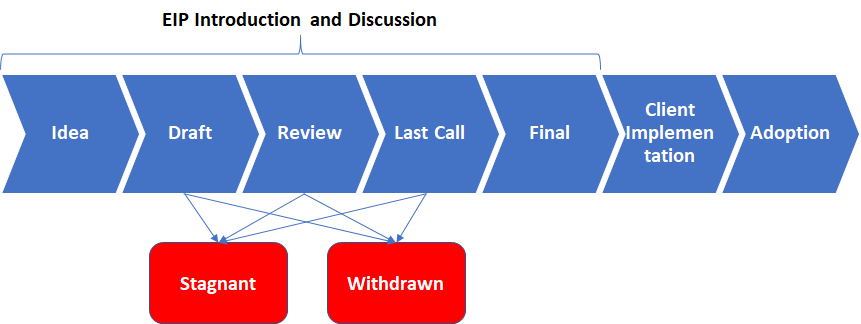
\includegraphics[width = 1\textwidth]{Figures/EIP_Process.png}}
    \label{EIP_process}
\end{figure}

\textit{EIP Introduction and Discussion:} The EIP process typically begins on a discussion board called Ethereum Research\footnote{See \url{https://ethresear.ch/}}, a forum for those interested to discuss ideas on how to change the Ethereum protocol. This venue serves as a sounding board for community feedback, and it is commonly used before an official EIP is created. Official proposals are then submitted via GitHub through a pull request, where an editor is tasked with ensuring adherence to format standards, acting as an archivist and moderator rather than a gatekeeper. The editor assigns a number to the EIP, and opens a dedicated channel on the Fellowship of Ethereum Magicians, the main forum to discuss EIPs. The EIP thus enters the Draft stage, where the proposal is further developed. When the authors, in agreement with the editor, are ready to receive feedback from the community, they move the EIP to the Review stage. The term ``editor'' may be misleading, particularly to an academic audience. There are no editorial decisions involved; anyone who wishes to write an EIP may do so, provided that the formatting standards and general structure of an EIP are met. EIP authors are responsible for shepherding the proposal to all stakeholders, listen to their comments, and address possible concerns. Venues for discussing include the Magicians discussion board, Ethereum conferences, developer calls, and social media servers like Discord. 

After the proposal is mature and stable, it is advanced to the Last Call stage, where the proposal is discussed in AllCoreDevs calls, a biweekly meeting held by the Ethereum developer community. Since Ethereum is not a membership organization, it does not vote, nor does it believe that voting is the best decision-making process. Instead, it follows the idea of ``rough consensus'', where proposals are advanced and finalized only when a large number of participants agree, and there is a general sense that the concerns of the dissenting party have been heard and considered. This does not necessarily require a unanimous agreement that the proposal is the best option. Instead, it signifies a consensus that it is ``good enough'' and that no specific concerns remain unaddressed.\footnote{See \cite{Resnick2014} for a detailed description of what rough consensus means.} Once a rough consensus is achieved, its status is updated to final. Once the proposal is final, it cannot be changed anymore.

Any proposal in the draft, review, and last call stages that lies dormant for six months enters a Stagnant stage, but can be revived, or formally withdrawn by its authors, if consensus cannot be reached, or if it is made redundant by other proposals. Withdrawn proposals cannot be resurrected. \footnote{Two additional stages, ``living'' (for continuously updated EIPs, exemplified by EIP 1, which establishes EIP standards and guidelines) and ``idea'' (for pre-draft proposals not formally tracked in the EIP repository), are excluded from our analysis.} 

\textit{EIP Implementation:}  EIPs can be divided into proposals that necessitate client software changes, and those that do not. EIPs are classified into 6 categories: ERCs, Interface, Core, Networking, Informational, and Meta. ERCs and Interface EIPs are related to creating a standard for specific applications and smart contracts, like EIP-20, which creates a standard for fungible tokens. These EIPs do not require any implementation in the client software. The finalization of such EIPs means that these standards have been approved by the Ethereum community. In theory, there is no need to go through the EIP process to create a standard, but it is good practice to do so to engage the community on the standard creation. Informational and Meta EIPs provide information about the governance process, and the software releases. 

All Core and Networking EIPs involve a change to the client software, and thus require the involvement of client developers. Ethereum currently has 4 main execution clients, written in 3 different programming language: Geth is by far the most popular client with 85\% of nodes running its implementation of the Ethereum protocol, written in the Go language. Nethermind and Besu are next, with both about 5\% of market share, written in C\# and Java, respectively. Erigon, with about 1\% of market share, was also written in Go.\footnote{Recently, Reth, a new client written in Rust, has gained some popularity. Reth is excluded from our analysis as the first alpha has only been released in June 2023. It therefore falls outside the observation period. Similarly, we are not considering deprecated clients.} Each client is an open source project with dedicated developers who often attend AllCoreDevs meetings, and participate in the governance process. Client developers work with EIP authors to implement proposals that they deem worthy. Technically, clients cannot be forced to implement all finalized EIPs. They are often constrained in their resources to implement changes to the software. Not implementing the same changes as other clients could lead to consensus issues and unintentional chain splits. Consequently, the client teams often work together with the community at large to find which finalized EIPs should be implemented first.

\textit{EIP Adoption:} Finally, once EIPs are implemented, a new client software version is released to the public, and node operators decide whether to upgrade. Major protocol upgrades historically occur through hard forks which are not backward compatible, meaning that if some nodes decide not to upgrade, they are left out of the peer-to-peer network. This means that all upgraded nodes will be part of a new network, and all the nodes that decide not to upgrade will be on another network, and the protocol splits. This has happened rarely in the history of Ethereum: The most controversial persistent chain split occurred during the DAO hacking event of June 2016, when the community decided to rewind a very large hacking attack, effectively re-writing its history. While many participants agreed to the change, some did not, and the protocol split into two networks: Ethereum and Ethereum Classic. 

Nodes are not the only entities deciding which version of the software to adopt. Other stakeholders influence whether to follow the recommended changes or not. For example, if the network splits into two forks, some service providers might decide to follow just one of the forks. For example, issuers of off-chain collateralized stablecoins have to choose only one of the forks, as a dollar of off-chain reserves cannot be backing two stablecoin tokens. Since stablecoins are an important component of the Ethereum ecosystem and used as collateral across numerous smart contract-based financial protocols, stablecoin issuers may have substantial influence on whether an upgrade is successful or not. Similarly, providers of external data, so-called oracles, might decide not to support an upgrade if they do not agree with the changes to the protocol. Since many smart contract-based financial protocols are dependent on these oracles, they will only ever work on a chain that is supported by the data provider. Consequently, oracle providers could hold effective veto power in the governance process. 

%%%%%%%%%%%%%%%%%%%%%%%%%%%%%%%%%%%%%%%%%%%%%%%%%%%%%%%%%%%%%%%%
%%%%%%%%%%%%%%%%%%%%%%%%%%%%%%%%%%%%%%%%%%%%%%%%%%%%%%%%%%%%%%%%
\subsection{Data} \label{subsec_data}
%%%%%%%%%%%%%%%%%%%%%%%%%%%%%%%%%%%%%%%%%%%%%%%%%%%%%%%%%%%%%%%%
%%%%%%%%%%%%%%%%%%%%%%%%%%%%%%%%%%%%%%%%%%%%%%%%%%%%%%%%%%%%%%%%

Ethereum is a permissionless platform not only because anyone can run client software and join the network, but also because it allows anyone to engage in the governance, and propose a change to the protocol. Most information about the protocol is accessible openly on the Ethereum GitHub page.\footnote{https://github.com/ethereum/} From there, we collect the list of all EIP numbers, titles, and authors as of June 21, 2023. A total of 612 EIPs have been submitted by 685 unique authors. The median EIP has 2 authors. Figure \ref{fig:neip_year} illustrates the growth in the number of EIPs and authors and the categorization of EIPs initiated each year.\footnote{In our study, we exclude EIPs labeled as ``Meta'' (21 EIPs) and ``Informational'' (6 EIPs) as they simply provide governance information, rather than proposals to actually change the protocol.} 

%%%%%%%%%%%%%%%%%%%%%%%%%%%%%%%%%%%%%%%%%%%%%%%%%%%%%%%
\begin{figure}[t!]
    \caption{Number of EIPs by Year}
     \begin{small}
    \begin{minipage}{\textwidth}
      This figure shows the number of EIPs by category (left axis) and the number of unique authors (right axis) over time. Year 2023 numbers are incomplete, as data collection ended on June 21, and are marked with an asterisk.
  \end{minipage}
         \end{small}
    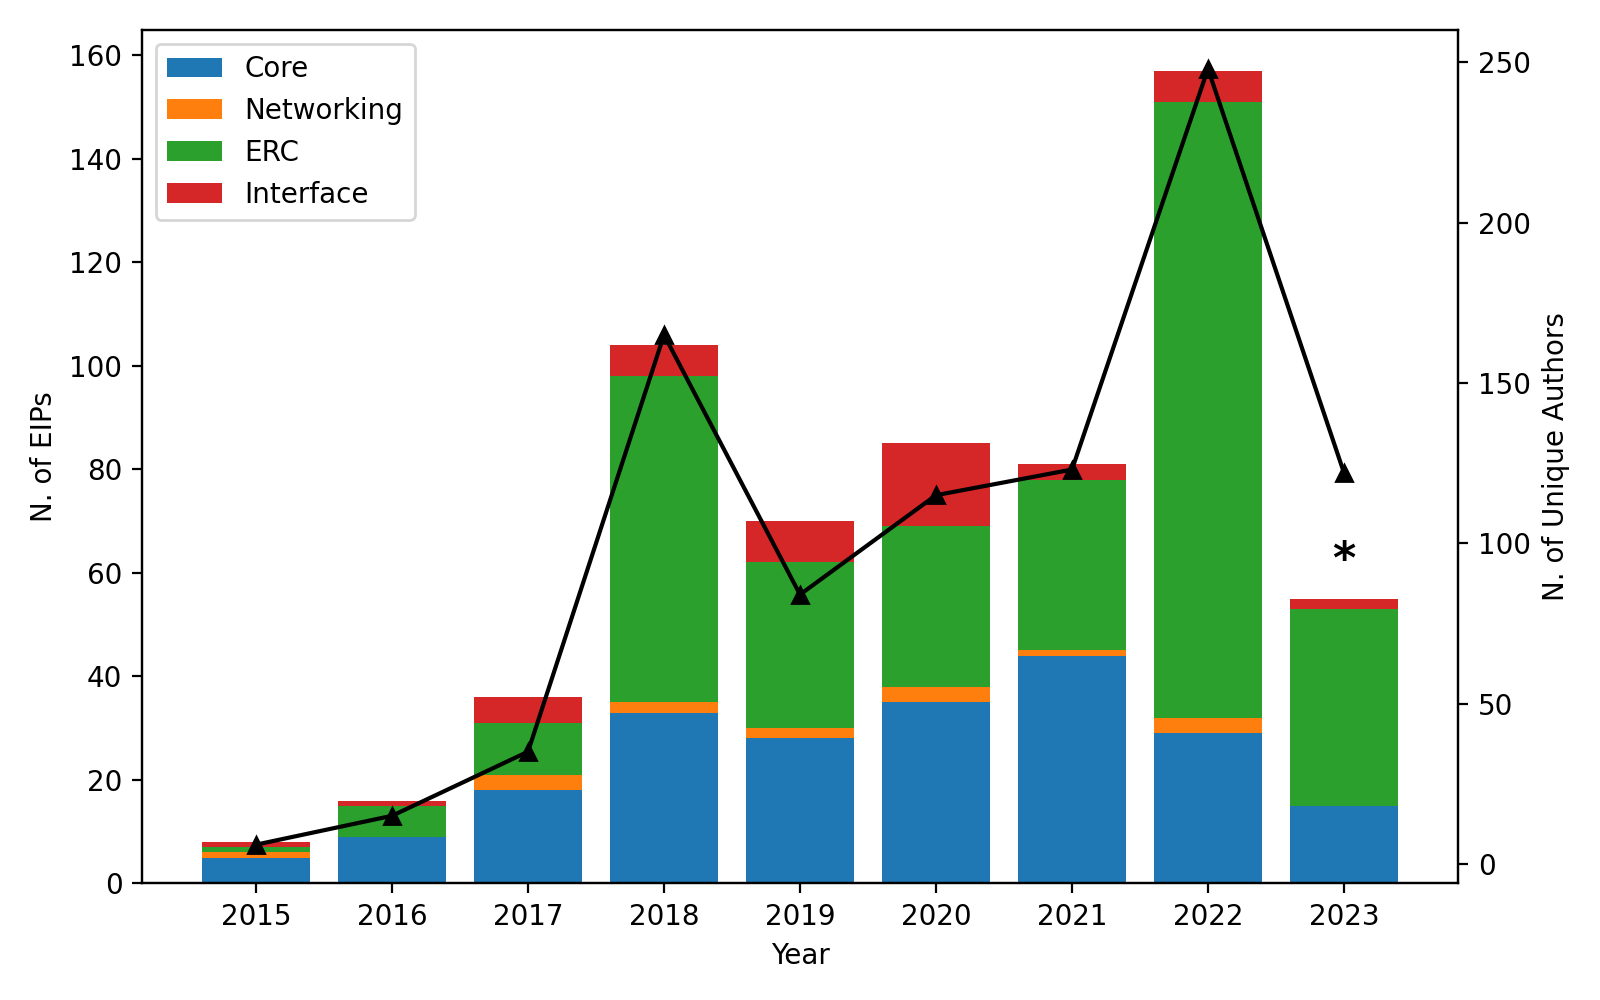
\includegraphics[width = \textwidth]{Figures/neip_by_year.png}
    \label{fig:neip_year}
\end{figure}
%\clearpage
%%%%%%%%%%%%%%%%%%%%%%%%%%%%%%%%%%%%%%%%%%%%%%%%%%%%%%%

54\% of all proposed EIPs are related to ERC standards, 35\% are Core EIPs that propose changes to the client software, and the rest are Interface and Networking related. Since Ethereum's early days, the total number of EIPs has grown steadily. ERC EIPs have gained recent popularity, while Core EIPs have remained relatively stable since 2018. Similarly, the number of authors has risen markedly, with over 250 individuals authoring an EIP in 2022. EIP discussions are also held in open venues, either on the ``Fellowship of Ethereum Magicians'' internet forum, or during AllCoreDevs calls. Proposals are also discussed in unofficial venues, like Ethereum conferences and Discord channels. Table \ref{summarystats} shows the summary statistics of the variables collected for the analysis.


%%%%%%%%%%%%%%%%%%%%%%%%%%%%%%%%%%%%%%%%%%%%%%%%%%%%%%%
%\begin{landscape}
\begin{table}
    \caption{Summary Statistics}
     \begin{small}
    \begin{minipage}{\textwidth}
      This table shows the summary statistics of the variables used in the paper. 
  \end{minipage}
         \end{small}
    \makebox[\textwidth][c]{{
\def\sym#1{\ifmmode^{#1}\else\(^{#1}\)\fi}
\begin{tabular}{l*{1}{rrrrrrrr}}
\hline\hline
                    &\multicolumn{8}{c}{}                                                                                   \\
                    &          N.&        Mean&    St. Dev.&         Min&         p25&         p50&         p75&         Max\\
\hline
Anonymous Author    &         610&       0.118&       0.323&           0&           0&           0&           0&           1\\
Finalized           &         431&       0.334&       0.472&           0&           0&           0&           1&           1\\
Implemented         &         178&       0.309&       0.463&           0&           0&           0&           1&           1\\
N. EIP Authors      &         605&       2.098&       1.545&           1&           1&           2&           3&          15\\
N. Twitter Followers (K)&         612&     348.704&   1,212.335&           0&        .436&        4.04&        13.3&       4,700\\
N. Github Followers &         612&   1,193.819&   2,785.890&           0&          25&         235&         743&      11,000\\
N. Words in EIP (k) &         612&       1.500&       1.272&        .087&        .648&        1.13&         1.9&        8.11\\
Readability Score   &         612&      39.061&      12.221&           0&          33&        39.8&          47&        76.8\\
\hline\hline
\end{tabular}
}
}
    \label{summarystats}

\end{table}
%\end{landscape}
%%%%%%%%%%%%%%%%%%%%%%%%%%%%%%%%%%%%%%%%%%%%%%%%%%%%%%%




%%%%%%%%%%%%%%%%%%%%%%%%%%%%%%%%%%%%%%%%%%%%%%%%%%%%%%%%%%%%%%%%
%%%%%%%%%%%%%%%%%%%%%%%%%%%%%%%%%%%%%%%%%%%%%%%%%%%%%%%%%%%%%%%%
%%%%%%%%%%%%%%%%%%%%%%%%%%%%%%%%%%%%%%%%%%%%%%%%%%%%%%%%%%%%%%%%
\section{The Effect of Ethereum Governance on Token Value}
%%%%%%%%%%%%%%%%%%%%%%%%%%%%%%%%%%%%%%%%%%%%%%%%%%%%%%%%%%%%%%%%
%%%%%%%%%%%%%%%%%%%%%%%%%%%%%%%%%%%%%%%%%%%%%%%%%%%%%%%%%%%%%%%%
%%%%%%%%%%%%%%%%%%%%%%%%%%%%%%%%%%%%%%%%%%%%%%%%%%%%%%%%%%%%%%%%

Establishing a clear link between governance actions and token price is a necessary precondition for the rest of our analysis: price-relevant information is what makes insider trading possible, contributor incentives meaningful, and regulatory classification relevant. Unlike traditional open-source communities, which rely uniquely on intrinsic motivation and reputational rewards, crypto governance affects a broad base of token holders with direct financial exposure to its outcomes. 

The governance structure of Ethereum is uniquely distinct from its native cryptocurrency, Ether. Unlike traditional companies where shareholders influence governance through voting and board elections, Ethereum's governance does not grant such power to Ether holders. Instead, anyone can participate in governance discussions, regardless of their Ether ownership. This approach, which operates off-chain without voting, contrasts with many DAOs where governance decisions are made through on-chain voting exclusive to token holders.

Ether's value is theoretically linked to Ethereum's governance, as it underpins a decentralized financial ecosystem aiming for accessibility, scalability, speed, and affordability. Every network-validated transaction incurs a fee payable in Ether, with a portion of this fee being ``burned,'' effectively reducing the Ether supply similar to a company's share repurchase. 

Analyzing Ethereum's governance effect on Ether's price poses two main empirical challenges. The first is selecting an appropriate benchmark for comparison. We use the S\&P 500 index and Bitcoin price as reference markets. The S\&P 500 offers a broad stock market perspective, but Ether's price has outpaced it over the sample period, with an average abnormal return of over 100\% per year. Comparing Ether and S\&P500 returns on random dates would thus provide an upward drift in Ether cumulative abnormal returns of about 10\% per month.  Bitcoin, having similar return levels to Ether, mitigates this drift, but the interconnected nature of the crypto market could mean that an improvement in Ethereum's prospects might spill over to the rest of the crypto-market, leading to underestimation of governance-related price responses.

The second challenge is Ethereum's transparent governance process, with few market-surprising announcements. Major decisions, like the transition from proof-of-work to proof-of-stake, unfolded over years with extensive public discussion, with multiple proposals, testnet implementations, and delays. Even single EIPs are openly proposed on GitHub, discussed in online forums, conferences, and in AllCoreDevs Calls. Updates to the EIP proposals and the client code are also visible in plain sight on GitHub. It is thus likely that the effect of an EIP proposal on Ether value is priced in gradually over time until it is finalized. 

Under the null that no information about an EIP's prospects is revealed before its final discussion, a conventional event-study design is appropriate: abnormal returns should be flat in the pre-event window and react sharply at the event itself. Under the alternative that information is released gradually and transparently, as the process described above suggests, the pre-event window itself becomes the object of interest: we should instead observe a run-up in abnormal returns beginning before the final discussion.
 
Our study focuses on Ether's price trend around the final discussions and approvals of successful Core EIPs. First, we collect hourly candles (open, close, min, max, and volume) from Coinbase's open API data feeds. \footnote{https://docs.cloud.coinbase.com/exchange/docs/welcome} The time-series data begins in May 2016 and ends in November 2023. Although cryptocurrencies trade 24/7, we compute daily returns using close prices at 4:00 pm Eastern US time during trading days when traditional financial markets are open, so that the Ether time-series data is aligned with the S\&P500. We then use the S\&P500 index and the Bitcoin prices as benchmarks to compute abnormal returns; Bitcoin's return series is restricted to this same set of trading days, so that the Ether, Bitcoin, and S\&P 500 series all share an identical calendar, with any price movement over a weekend or market holiday folded into the return of the following trading day. 

For each EIP, we identify the last AllCoreDevs Call in which developers meet to discuss and approve the proposal. We identified 41 out of 51 finalized Core EIPs. Table \ref{tab:car_event_study} and Figure \ref{fig:CAR} show the cumulative abnormal returns (CARs) in the red line, and the 90\% confidence interval in the gray shaded area, on a window of [-40;+40] trading days around the call. Panel (a) uses as reference the S\&P500 index, and panel (b) Bitcoin. 
 
The findings reveal a price increase beginning about 30 trading days before a Core EIP's final discussion. As expected, when benchmarked against the S\&P 500, Ether's excess returns over the sample period display a drift, making quantitative assessment of the influence of governance on prices challenging. Still, removing a 10\% drift per month, one can notice a run-up in price that begins about a month prior to the approval of the core EIP. To make a more precise assessment, we use Bitcoin as reference. We observe a 13.2\% price run-up in the 25 days preceding a Core EIP approval. 

These findings show that the Ethereum governance, and the process of improving the protocol and thus the speed, security, and costs of operating on the platform, has a material impact on the value of the Ether token. This has direct implications both for investors, as we show that crypto returns are driven by governance decisions, and for regulators, as the impact of governance on token value is an important condition for disclosure and supervisory regimes. 


%%%%%%%%%%%%%%%%%%%%%%%%%%%%%%%%%%%%%%%%%%%%%%%%%%%%%%%
\begin{figure}[ht!]
    \caption{Ethereum Governance and Token Price}
     \begin{small}
    \begin{minipage}{\textwidth}
      This figure shows the Cumulative Abnormal Returns (CARs) of Ether prices in a [-40;+40] trading day window around the last AllCoreDevs Call where a Core EIP is discussed. Panel (a) uses the S\&P500 as reference, and panel (b) uses Bitcoin.  
     \end{minipage}
         \end{small}
         \\[0.5cm]
   \begin{subfigure}{0.49\textwidth}
           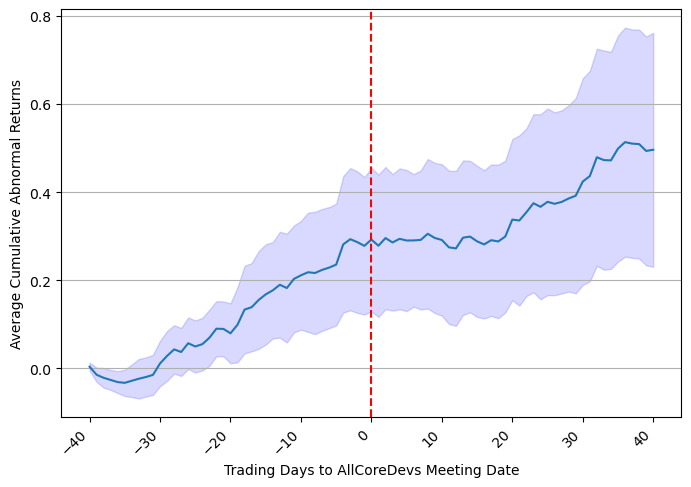
\includegraphics[width = 1\textwidth]{Figures/CAR_SPY.png}
            \caption{Benchmark: S\&P500 }
            \label{fig:CARSPY}
   \end{subfigure}
   \begin{subfigure}{0.49\textwidth}
           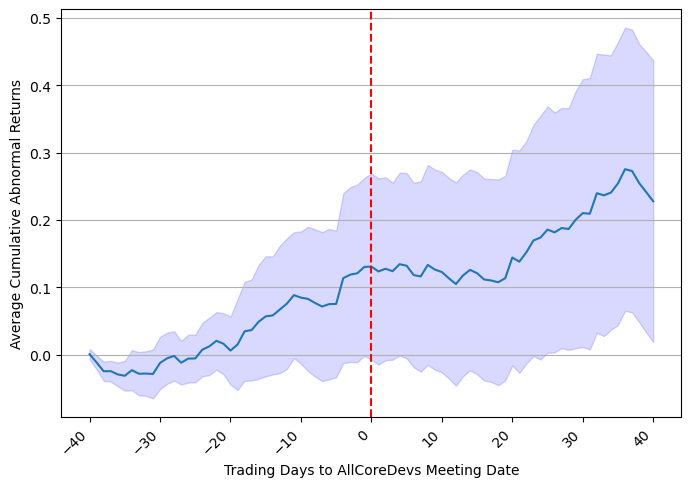
\includegraphics[width = 1\textwidth]{Figures/CAR_BTC.png}
            \caption{Benchmark: Bitcoin}
            \label{fig:CARBTC}
   \end{subfigure}
  
    \label{fig:CAR}
\end{figure}

%%%%%%%%%%%%%%%%%%%%%%%%%%%%%%%%%%%%%%%%%%%%%%%%%%%%%%%
\begin{table}[ht!]
    \caption{Cumulative Abnormal Returns around AllCoreDevs Discussion of Finalized Core EIPs}
     \begin{small}
    \begin{minipage}{\textwidth}
      This table reports the mean cumulative abnormal return (CAR) of Ether at selected trading-day horizons around the last AllCoreDevs meeting discussing each finalized Core EIP, benchmarked against the S\&P 500 (column 1) and Bitcoin (column 2), corresponding to Figure \ref{fig:CAR}. Standard errors, reported in parentheses, are computed across events at each horizon. *, **, and *** indicate statistical significance at the 10\%, 5\%, and 1\% levels, respectively.
  \end{minipage}
         \end{small}
    \makebox[\textwidth][c]{% ===== Table: CAR event-study estimates (SPY and BTC benchmarks) =====
% Companion to Figure \ref{fig:CAR}: same estimates, selected horizons, tabular form.
\begin{tabular}{lcc}
\toprule
 & CAR (S\&P 500 benchmark) & CAR (Bitcoin benchmark) \\
\midrule
\quad $t=-40$ & 0.004 & 0.001 \\
 & (0.006) & (0.005) \\
\quad $t=-35$ & -0.033$^{*}$ & -0.031$^{**}$ \\
 & (0.018) & (0.013) \\
\quad $t=-30$ & 0.011 & -0.012 \\
 & (0.031) & (0.024) \\
\quad $t=-25$ & 0.050 & -0.005 \\
 & (0.036) & (0.022) \\
\quad $t=-20$ & 0.079$^{*}$ & 0.006 \\
 & (0.041) & (0.031) \\
\quad $t=-15$ & 0.168$^{**}$ & 0.057 \\
 & (0.069) & (0.054) \\
\quad $t=-10$ & 0.211$^{***}$ & 0.085 \\
 & (0.075) & (0.060) \\
\quad $t=-5$ & 0.235$^{***}$ & 0.076 \\
 & (0.084) & (0.066) \\
\quad $t=-1$ & 0.278$^{***}$ & 0.130 \\
 & (0.095) & (0.080) \\
\quad $t=0$ (Final Discussion Date) & 0.292$^{***}$ & 0.131 \\
 & (0.099) & (0.084) \\
\quad $t=+1$ & 0.278$^{***}$ & 0.124 \\
 & (0.098) & (0.084) \\
\quad $t=+5$ & 0.290$^{***}$ & 0.132 \\
 & (0.097) & (0.084) \\
\quad $t=+10$ & 0.291$^{***}$ & 0.123 \\
 & (0.105) & (0.090) \\
\quad $t=+15$ & 0.288$^{***}$ & 0.121 \\
 & (0.104) & (0.091) \\
\quad $t=+20$ & 0.338$^{***}$ & 0.144 \\
 & (0.111) & (0.097) \\
\quad $t=+25$ & 0.378$^{***}$ & 0.186 \\
 & (0.129) & (0.111) \\
\quad $t=+30$ & 0.424$^{***}$ & 0.210$^{*}$ \\
 & (0.143) & (0.121) \\
\quad $t=+35$ & 0.499$^{***}$ & 0.254$^{*}$ \\
 & (0.156) & (0.128) \\
\quad $t=+40$ & 0.496$^{***}$ & 0.228$^{*}$ \\
 & (0.161) & (0.127) \\
\midrule
Observations (events) & 41 & 41 \\
\bottomrule
\end{tabular}
}
    \label{tab:car_event_study}
\end{table}
%%%%%%%%%%%%%%%%%%%%%%%%%%%%%%%%%%%%%%%%%%%%%%%%%%%%%%%



%%%%%%%%%%%%%%%%%%%%%%%%%%%%%%%%%%%%%%%%%%%%%%%%%%%%%%%%%%%%%%%%
%%%%%%%%%%%%%%%%%%%%%%%%%%%%%%%%%%%%%%%%%%%%%%%%%%%%%%%%%%%%%%%%
%%%%%%%%%%%%%%%%%%%%%%%%%%%%%%%%%%%%%%%%%%%%%%%%%%%%%%%%%%%%%%%%
\section{The Effect of Governance Proposals on Labor Market Outcomes} \label{sec:labor}
%%%%%%%%%%%%%%%%%%%%%%%%%%%%%%%%%%%%%%%%%%%%%%%%%%%%%%%%%%%%%%%%
%%%%%%%%%%%%%%%%%%%%%%%%%%%%%%%%%%%%%%%%%%%%%%%%%%%%%%%%%%%%%%%%
%%%%%%%%%%%%%%%%%%%%%%%%%%%%%%%%%%%%%%%%%%%%%%%%%%%%%%%%%%%%%%%%

The financial incentives associated with token holdings, discussed in the previous section, are a first-order consideration for governance participants, who often accumulate large token grants and holdings over the course of their involvement. Many of these volunteers also hold full-time positions at companies operating in the Ethereum ecosystem, and so already face financial incentives set by their employers. However, financial incentives are not the only channel through which contributors are rewarded for their effort. Like any OSC, Ethereum's governance process has no formal employment relationship: authors of an Ethereum Improvement Proposal (EIP) are volunteers, not employees of the protocol. A traditional explanation for sustained participation in open-source communities is the signaling channel formalized by \cite{Spence1973}: in a labor market where employers cannot directly observe a worker's underlying ability, individuals take costly, observable actions to credibly reveal private information about their quality. Authoring an EIP is exactly this kind of costly signal, requiring specialized technical knowledge and subjecting the author's work to public scrutiny by the developer community. We would therefore expect that proposing an EIP allows contributors to signal both their skill and their visibility within the ecosystem, improving their subsequent career prospects along two dimensions: the seniority of their employment and their compensation. Revelio Labs' Seniority is an ordinal variable with 7 discrete levels (Entry/Intern through Senior Executive) that is predicted from a worker's title, industry, company size, job-history patterns, and position tenure.

To test this hypothesis, we collect career history data from Revelio Labs, a provider of professional profile data that tracks employment transitions, job titles, and estimated compensation. We match 469 of all EIP authors (68.5\% of the authors in our sample) to a Revelio profile, and construct a panel tracking each matched author's seniority level and estimated compensation in each year surrounding their EIP proposal.

We consider each author's proposal of an EIP as a treatment event occurring at time $t=0$ as long as the person has not authored any in
the preceding two years, and match each treated author to at most three control authors. Matching is performed on pre-event seniority and on Mahalanobis distance over log compensation in the pre-period, using a $\chi^2(0.90)$ caliper, and control authors are required to have proposed no EIP of their own within the $[-2,+2]$ window. Each treated author together with their three matched controls forms a cohort, observed over a window of $[-2,+2]$ years around the proposal year. We then stack all cohorts together and estimate a generalized stacked difference-in-differences model.

\begin{equation}
\begin{split}   
  Y_{i,c,t}  =& \alpha_0 + \alpha_1 D_{i,c} * P_{t,c} + \gamma_{i,c} + \delta_{t,c} +  \epsilon_{i,c,t}  \label{eq:labor}
\end{split}
\end{equation}

where $Y_{i,c,t}$ is the seniority or total compensation (log) of author $i$ in cohort $c$ at time $t$. $D_{i,c}$ is a dummy equal to one if the author proposes an EIP at time $t=0$. $P_{t,c}$ is a dummy equal to 1 if $t\geq0$. $\gamma_{i,c}$ and $\delta_{t,c}$ are author-cohort and time-cohort fixed effects. In addition to this static specification, we also estimate a dynamic version of the model, replacing the single post-treatment indicator $P_{t,c}$ with a full set of indicators for each year relative to the proposal, allowing the treatment effect to vary flexibly across the $[-2,+2]$ event window. This dynamic specification lets us trace the evolution of the effect over time and visually assess pre-trends in the years leading up to the EIP proposal. Standard errors are clustered at the author level.

Our identification relies on the assumption that the timing of an author's EIP proposal is orthogonal to their subsequent labor market outcomes. We provide two pieces of evidence in support of this assumption. First, because treated and control authors are matched on seniority and compensation in both pre-event years, they exhibit similar levels and pre-trends on the very outcomes we study. Second, and more informative, treated and matched control authors also look similar the year before the EIP proposal along a wide range of characteristics that play no role in the matching procedure, as shown in Panel A of Table \ref{tab:did_main}. This balance on characteristics excluded from the matching procedure is suggestive that unobservable characteristics are similarly balanced across the two groups, and that our identifying assumption is not invalidated by systematic differences between authors who choose to propose an EIP in a given year and those who do not.

Panel B of Table \ref{tab:did_main} presents the diff-in-diff estimates for seniority. Column (1) shows that, on average, seniority rises by 0.22 notches following EIP proposal, a 6\% increase relative to the sample mean. Column (2), together with panel (a) of Figure \ref{fig:labor}, reports the dynamic specification. By construction, the pre-trend is flat, since authors are matched on pre-EIP seniority levels. The effect emerges quickly and grows over time: seniority rises by 0.2 notches by the end of the calendar year in which the EIP is introduced, and reaches almost 0.3 notches two years out. This rapid response may seem surprising, but it likely reflects the fact that event time, defined here by the EIP's formal introduction, understates when the underlying signal actually begins: EIPs are typically preceded by extensive discussion in venues such as Ethereum Research (\url{https://ethresear.ch/}), so the true starting point of the signal probably precedes our measured event date. \footnote{As a robustness check, we repeat the analysis at a quarterly frequency and obtain similar results.}


% ===== Table: covariate balance + difference-in-differences results =====

\begin{center}
\begin{table}
 \caption{The Effect of EIP Authorship on Seniority and Compensation} \label{tab:did_main}
     \begin{small}
    \begin{minipage}{\textwidth}
      The table reports covariate balance and difference-in-differences estimates of the effect of authoring an Ethereum Improvement Proposal (EIP) on career outcomes over a
$\pm2$-year event window. An author is treated if they propose an EIP at t=0. Each treated author is matched to at most three similar control
authors drawn from the population of EIP authors who author no EIP anywhere in the $\pm2$-year window; Panel A shows the results of a balance test. Panel B and C report stacked diff-in-diff results for Seniority and Total Compensation (log) as outcome variable. Column~(1) reports the static model. Column~(2) replaces it with separate coefficients for each event year, $t-1$ omitted as the reference. Columns~(3) and~(4)
re-run column~(1) on the two halves of the sample, split at the median of seniority in the year before authorship. Standard errors, reported in parentheses, are clustered at the author level;  $^{*}$, $^{**}$, and $^{***}$ denote statistical significance at the 10\%, 5\%, and 1\% levels, respectively.
  \end{minipage}
         \end{small}
\begin{tabular}{lcccccc}
\\

\multicolumn{5}{l}{\textbf{Panel A. Covariate Balance (at $t-1$)}} \\[2pt]
\toprule
 & \multicolumn{2}{c}{Mean} & & & & \\
\cmidrule(lr){2-3}
Variable & Treated & Control & Difference  & $p$-value \\
 & (1) & (2) & (3) & (4) \\
\midrule
\multicolumn{7}{l}{\textit{Variables used in matching}} \\
\quad Seniority (1--7) & 3.876 & 3.835 & 0.041  & 0.735 \\
\quad Total compensation (USD) & \$194,759 & \$189,813 & \$4,946 &  0.703 \\
\addlinespace
\multicolumn{7}{l}{\textit{Variables not used in matching}} \\
\quad School prestige score & 0.530 & 0.521 & 0.009 &  0.704 \\
\quad Education level (1--5) & 3.594 & 3.616 & -0.022 &0.703 \\
\quad Log base salary & 11.409 & 11.416 & -0.007 & 0.880 \\
\quad Engineering occupation & 64.0\% & 68.1\% & -4.0\% &  0.179 \\
\quad Female & 7.0\% & 8.0\% & -1.0\% &  0.547 \\
\quad Ethnicity: White & 70.8\% & 68.1\% & 2.7\%  & 0.348 \\
\quad Based in United States & 31.5\% & 33.4\% & -1.9\% & 0.507 \\
\quad Job located in North America & 43.3\% & 47.5\% & -4.2\% &  0.177 \\
\quad Employer identified in data & 91.0\% & 90.2\% & 0.9\% & 0.641 \\
\quad 500+ LinkedIn connections & 33.4\% & 36.3\% & -2.8\% &  0.341 \\
\midrule
Observations & 356 & 874 & &  \\
\bottomrule
\end{tabular}
\vspace{10pt}
\begin{tabular}{lcccc}
\multicolumn{5}{l}{\textbf{Panel B. Seniority (1--7)}} \\[2pt]
\toprule
 & (1) & (2) & (3) & (4) \\
 & \multicolumn{2}{c}{Full sample} & \multicolumn{2}{c}{By pre-event seniority} \\
\cmidrule(lr){2-3} \cmidrule(lr){4-5}
 & Static & Dynamic & Junior & Senior \\
 & & & \small(1--3) & \small(4--7) \\
\midrule
\quad Treated $\times$ Post ($t\geq 0$) & 0.221$^{***}$ &  & 0.284$^{**}$ & 0.150 \\
 & (0.083) &  & (0.112) & (0.124) \\
\addlinespace
\quad Treated $\times$ $t=-2$ &  & 0.000 &  &  \\
\quad Treated $\times$ $t=-1$ & & --- & & \\
\quad Treated $\times$ $t=+0$ &  & 0.190$^{**}$ &  &  \\
 &  & (0.080) &  &  \\
\quad Treated $\times$ $t=+1$ &  & 0.193$^{*}$ &  &  \\
 &  & (0.099) &  &  \\
\quad Treated $\times$ $t=+2$ &  & 0.282$^{***}$ &  &  \\
 &  & (0.106) &  &  \\
\midrule
Author $\times$ cohort FE & Yes & Yes & Yes & Yes \\
Cohort $\times$ event-time FE & Yes & Yes & Yes & Yes \\
Observations & 6,073 & 6,073 & 3,263 & 2,810 \\
\bottomrule
\end{tabular}
\end{table}
\nomarkersintext
\begin{table}[t]
\vspace{-9cm}
\begin{tabular}{lcccc}
\multicolumn{5}{l}{\textbf{Panel C. Log compensation}} \\[2pt]
\toprule
 & (1) & (2) & (3) & (4) \\
 & \multicolumn{2}{c}{Full sample} & \multicolumn{2}{c}{By pre-event seniority} \\
\cmidrule(lr){2-3} \cmidrule(lr){4-5}
 & Static & Dynamic & Junior & Senior \\
 & & & \small(1--3) & \small(4--7) \\
\midrule
\quad Treated $\times$ Post ($t\geq 0$) & 0.090$^{**}$ &  & 0.093$^{*}$ & 0.085 \\
 & (0.039) &  & (0.050) & (0.060) \\
\addlinespace
\quad Treated $\times$ $t=-2$ &  & -0.024 &  &  \\
 &  & (0.017) &  &  \\
\quad Treated $\times$ $t=-1$ & & --- & & \\
\quad Treated $\times$ $t=+0$ &  & 0.051 &  &  \\
 &  & (0.035) &  &  \\
\quad Treated $\times$ $t=+1$ &  & 0.077 &  &  \\
 &  & (0.048) &  &  \\
\quad Treated $\times$ $t=+2$ &  & 0.105$^{**}$ &  &  \\
 &  & (0.052) &  &  \\
\midrule
Author $\times$ cohort FE & Yes & Yes & Yes & Yes \\
Cohort $\times$ event-time FE & Yes & Yes & Yes & Yes \\
Observations & 6,073 & 6,073 & 3,263 & 2,810 \\
\bottomrule
\end{tabular}
\end{table}
\markersintext
\end{center}



\begin{figure}[p]
\centering
\begin{subfigure}[b]{0.48\textwidth}
    \centering
    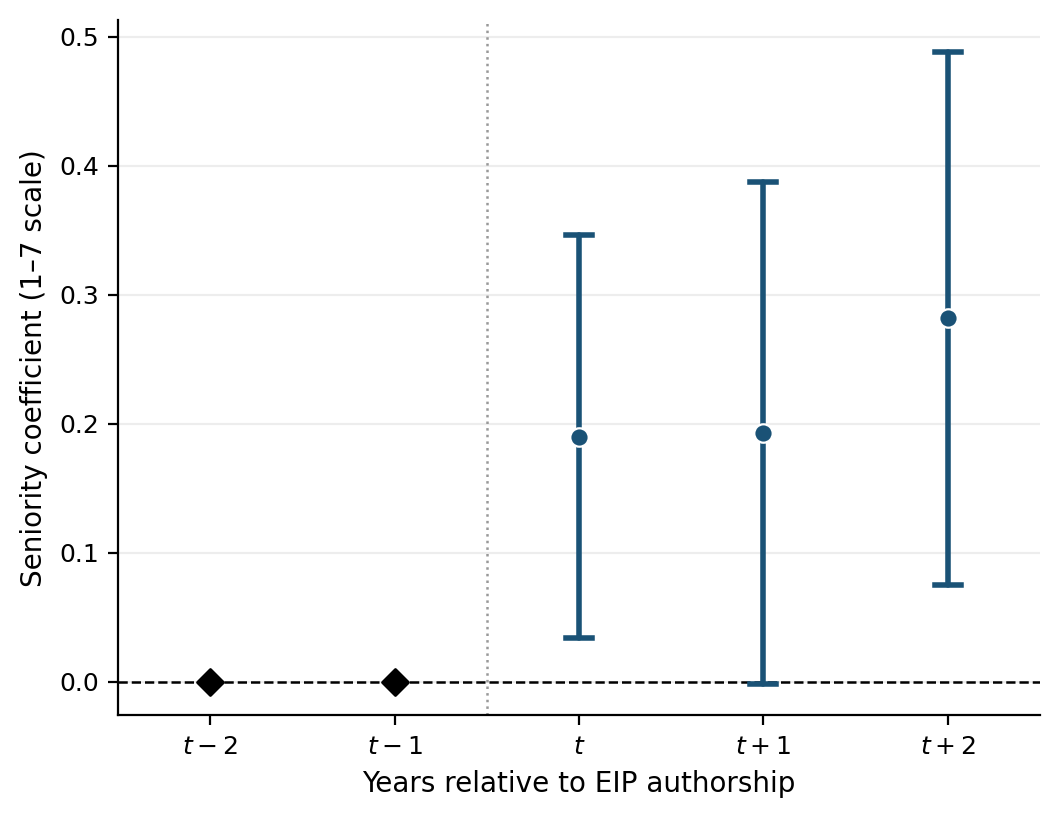
\includegraphics[width=\textwidth]{Figures/EIP_W2_EventStudy_Seniority.png}
    \caption{Seniority}
    \label{fig:sub_a}
\end{subfigure}
\hfill
\begin{subfigure}[b]{0.48\textwidth}
    \centering
    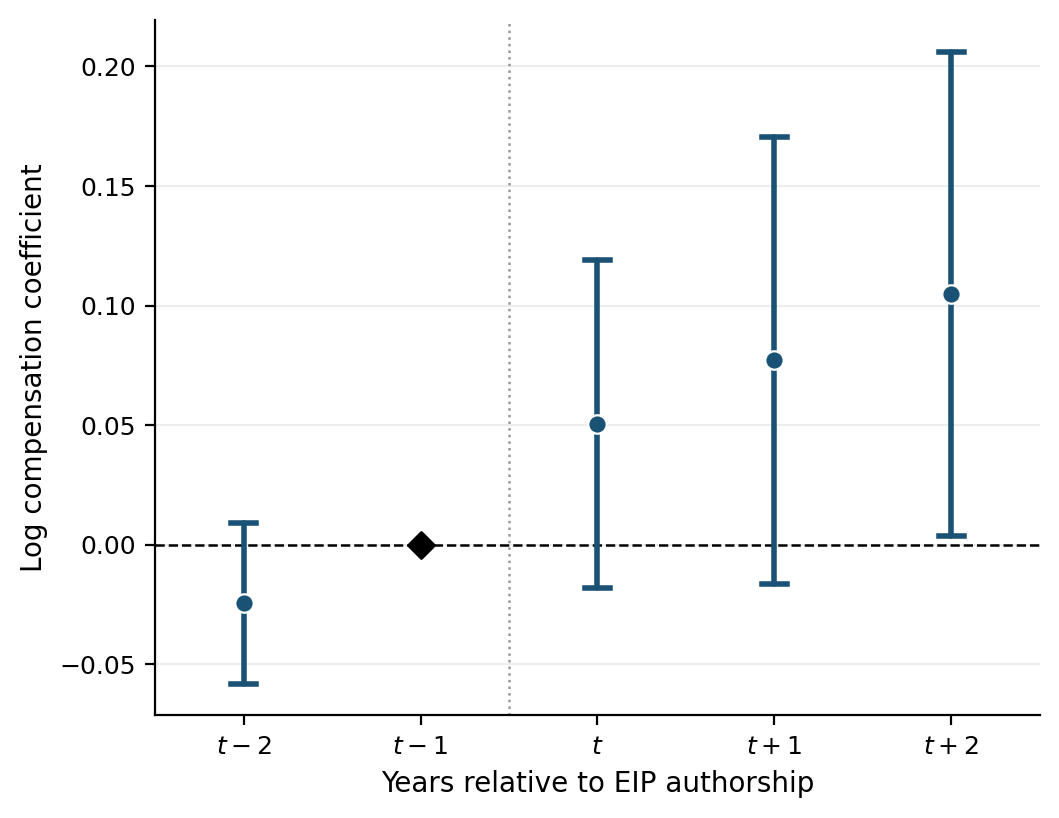
\includegraphics[width=\textwidth]{Figures/EIP_W2_EventStudy_LogComp.png}
    \caption{Total Compensation (log)}
    \label{fig:sub_b}
\end{subfigure}
\caption{The figure shows the coefficients of the stacked diff-in-diff equation \ref{eq:labor} dynamic specification, where the outcome variable is Seniority (a) and log of Total Compensation (b). Markers denote point estimates and vertical bars denote 95\% confidence intervals based on standard errors clustered at the author level.}
\label{fig:labor}
\end{figure}

Under the signaling hypothesis, information asymmetries are greatest for authors in more junior roles, so the labor market effects of proposing an EIP should be correspondingly larger for this group. To test this, we split the sample into Junior (Seniority $<$ 4 at $t=-1$) and Senior (Seniority $\geq$ 4) median subgroups and re-estimate the model separately for each. Columns (3) and (4) show that the effect is nearly twice as large for junior authors as for senior ones, confirming that authors benefit from authoring EIPs through an improvement in their labor careers.

We then repeat the analysis using total compensation (log) as outcome variable. While compensation is not disclosed on LinkedIn, Revelio Labs uses machine learning models trained on self-reported data and public employment records, and using features like company, role, seniority, and location to predict a salary distribution for each position, then separately estimates total compensation as a multiplier on that predicted base salary. Panel C of Table \ref{tab:did_main} shows the results using the same specifications of Panel B. Total compensation increases by 9\% after the introduction of an EIP, relative to other EIP authors who did not propose an EIP at that time. Column (2) and panel (b) of Figure \ref{fig:labor} show that the increase is gradual, peaking at 10.5\% two years out. Albeit smaller than in panel B, we find that the compensation of authors with junior roles are marginally larger than authors with senior roles. 

Overall, the analysis supports the signaling hypothesis that EIP contributors have indirect benefits associated with participating in Ethereum governance. Upon the proposal of an EIP, authors are promoted to more senior roles and receive greater compensation, particularly if they held junior roles beforehand. These results speak to the incentives that participants have in contributing to maintaining and improving the protocol. We view this as a desirable feature of the governance process rather than a source of concern: the existence of tangible labor-market returns to participation helps align contributors' individual incentives with the protocol's long-term needs, encouraging sustained engagement rather than one-off contributions. At the same time, this also implies that the governance process may be disproportionately shaped by contributors with the greatest reputational and career stake in its outcomes: those most responsive to labor-market incentives are also often the least established.



%%%%%%%%%%%%%%%%%%%%%%%%%%%%%%%%%%%%%%%%%%%%%%%%%%%%%%%%%%%%%%%%
%%%%%%%%%%%%%%%%%%%%%%%%%%%%%%%%%%%%%%%%%%%%%%%%%%%%%%%%%%%%%%%%
%%%%%%%%%%%%%%%%%%%%%%%%%%%%%%%%%%%%%%%%%%%%%%%%%%%%%%%%%%%%%%%%
\section{Transparency and Openness of Ethereum Governance} \label{sec:transparency}
%%%%%%%%%%%%%%%%%%%%%%%%%%%%%%%%%%%%%%%%%%%%%%%%%%%%%%%%%%%%%%%%
%%%%%%%%%%%%%%%%%%%%%%%%%%%%%%%%%%%%%%%%%%%%%%%%%%%%%%%%%%%%%%%%
%%%%%%%%%%%%%%%%%%%%%%%%%%%%%%%%%%%%%%%%%%%%%%%%%%%%%%%%%%%%%%%%

We then turn to the third test related to the extent of asymmetric or insider information in the Ethereum governance process. If all or most information is publicly available, concerns about insider trading and disclosure requirements should be greatly alleviated.   

Open source communities are known to have a high level of transparency. This is not simply a necessity to effectively collaborate on a global scale, but also part of a cultural ethos based on the belief that openness and transparency generate positive externalities. We thus proceed to assess the level of access and transparency of the Ethereum governance process. We use three main measures: the availability and technicality of the Ethereum protocol documents and code, the anonymity of the participants, and the transparency of the Ethereum Foundation. 

First, we look at the availability and technicality of the documents and proposals. While it is plausible that unobservable, private discussions occur among some developers (e.g., through Telegram chats or closed-door meetings), most discussions occur in official venues. The first forum to discuss possible protocol changes is Ethereum Research, an official open discussion platform dedicated to the advancement of Ethereum's core technology and protocol design. It serves as a collaborative hub where developers, academics, and cryptographers propose, debate, and refine ideas about protocol upgrades. After an EIP is drafted, it enters a circulation phase that includes three primary channels for community engagement and discussion. The first is the Fellowship of Ethereum Magicians (FEM) internet forum, followed by a repository on Github where participants can directly comment on the text of the proposed EIP, and AllCoreDevs Meetings, biweekly calls between authors, contributors, and client developers live streamed where core proposals that are closed to be finalized are discussed in an open, live-streamed venue. 

Overall, we conclude that the EIP process is open and transparent, particularly when compared to more traditional private and public companies where detailed disclosure about governance decision making is generally unavailable.

While the information about protocol upgrades is for the most part publicly available, individuals need to thoroughly understand the associated documentation and code. However, this can be challenging for those without a technical background. To gauge the extent to which people can understand EIPs, we have analyzed the length and readability of each EIP using the Flesch Reading Ease scale. This scale rates texts on a spectrum from 0 (least readable) to 100 (most readable) taking into account the number of words in a sentence, and the number of syllables in words. Our findings, illustrated in Figure \ref{fig:understand}, reveal that the average EIP scores 39.1 in readability, with a standard deviation of 12.2, as shown in table \ref{summarystats}. Scores in the 30-50 range typically indicate that a college-level understanding is necessary for comprehension. As a frame of reference, this paper has a readability score of 43.5, and computer science papers have an average readability score of 40.1  \citep{VainshteinEtAl2019}. While this may be expected for technical documents, a push for greater clarity in EIPs could help make them more accessible to a broader audience. Also, the average text length is 1,500 words, which is similar to typical scientific publications and articles. 

%%%%%%%%%%%%%%%%%%%%%%%%%%%%%%%%%%%%%%%%%%%%%%%%%%%%%%%
\begin{figure}[ht!]
    \caption{EIP Readability}
     \begin{small}
    \begin{minipage}{\textwidth}
      Panel (a) shows the histogram of the Flesch Reading Ease readability score applied to EIP texts. The score takes into account the number of words in a sentence, and the number of syllables in words. Panel (b) shows the histogram of the length of EIP texts, measured as the number of words (,000s).   
     \end{minipage}
         \end{small}
          \\[0.5cm]
   \begin{subfigure}{0.49\textwidth}
           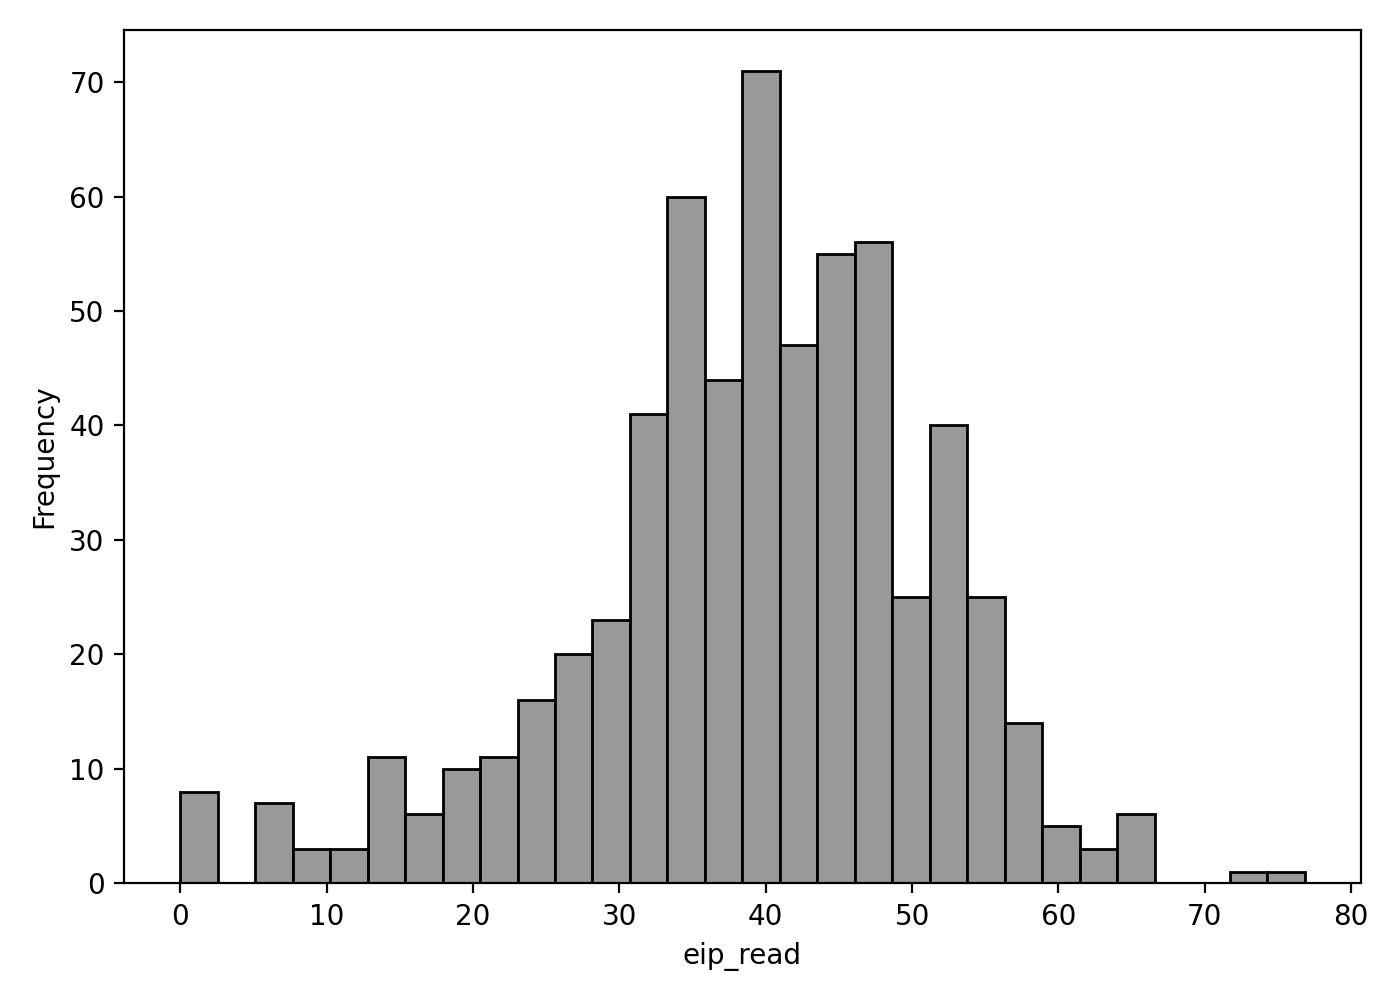
\includegraphics[width = 1\textwidth]{Figures/read_hist.png}
            \caption{EIP Readability Score}
            \label{fig:read}
   \end{subfigure}
    \begin{subfigure}{0.49\textwidth}
           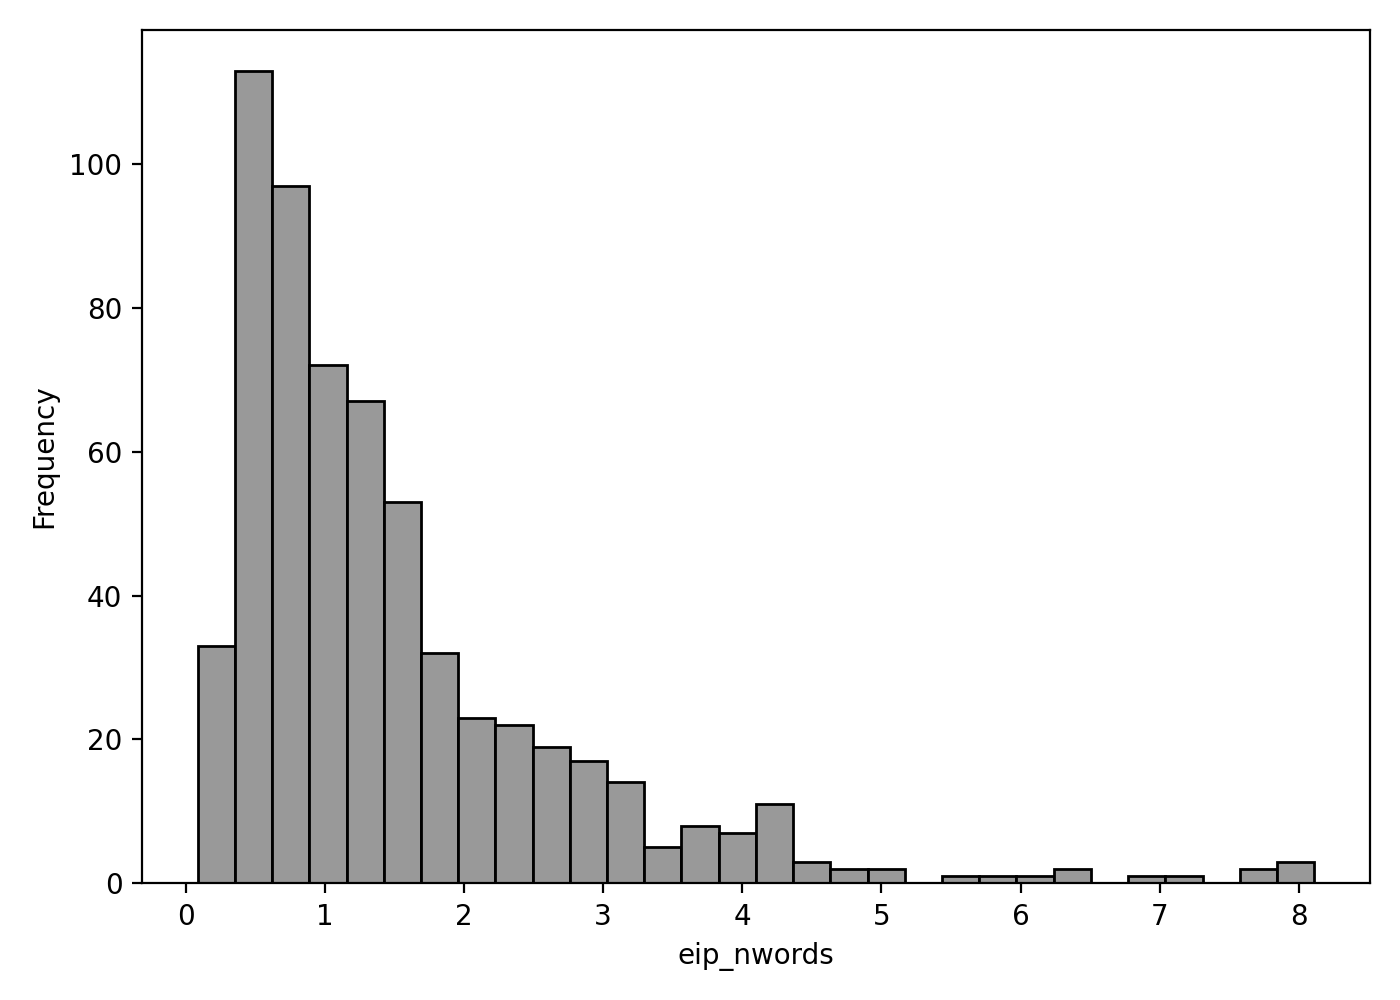
\includegraphics[width = 1\textwidth]{Figures/nwords_hist.png}
            \caption{EIP Length}
            \label{fig:nword}
   \end{subfigure}
    \label{fig:understand}
\end{figure}
%%%%%%%%%%%%%%%%%%%%%%%%%%%%%%%%%%%%%%%%%%%%%%%%%%%%%%%

Finally, we turn to the issue of anonymity. A common concern in the cryptocurrency sector is that projects are occasionally developed by anonymous bad actors that proceed to abscond with users' funds through what are called rug pulls. The lack of identity verification hinders law enforcement from pursuing charges against these criminals. Anonymity also prevents third parties from pursuing legal claims against responsible individuals in case of negligence or malfeasance. A fully transparent ecosystem includes not only the disclosure and availability of relevant discussions and documents, but also information about their contributors to assess potential conflicts of interest. We thus measure how many contributors in the Ethereum governance process disclose their full names. Figure \ref{fig:anon} shows that 89\% of EIP authors disclose their identity, 79\% of attendees of AllCoreDevs meetings, and 80\% of top client developers. A potential issue is that we do not have the ability to confirm whether their disclosed names match their true identity. We thus proceed to search for their social media accounts, to verify their real identity, and to use their employment information for further tests. We are able to find 75\% of EIP authors who disclose their full names on X, and 72\% on LinkedIn.      

%%%%%%%%%%%%%%%%%%%%%%%%%%%%%%%%%%%%%%%%%%%%%%%%%%%%%%%
\begin{figure}[ht!]
    \caption{Anonymity in the Ethereum Governance Process}
     \begin{small}
    \begin{minipage}{\textwidth}
      This figure shows the percentage of people disclosing their full names in EIP proposals, AllCoreDevs meetings, and Github Client commits for the top 20 most prolific developers.    
     \end{minipage}
         \end{small}
         \\[0.5cm]
    \makebox[\textwidth][c]{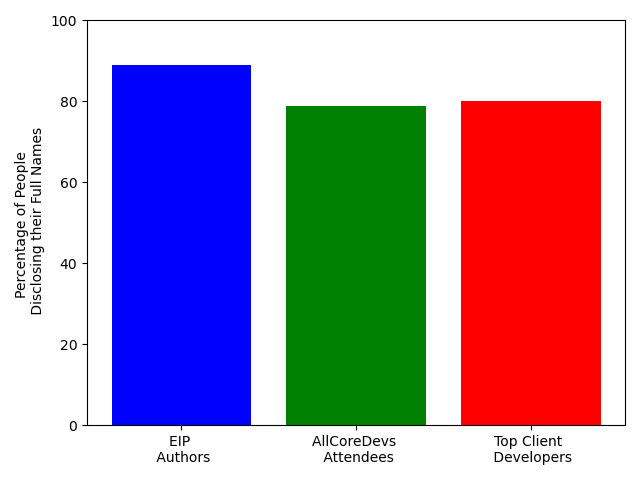
\includegraphics[width = 0.8\textwidth]{Figures/Anonymity_Diagram.png}}
    \label{fig:anon}
\end{figure}
%%%%%%%%%%%%%%%%%%%%%%%%%%%%%%%%%%%%%%%%%%%%%%%%%%%%%%%


Many companies and non-profits engage with the Ethereum governance process. By the nature of their businesses, these companies are not as transparent as the Ethereum governance process. However, one organization stands out among many for its special role within the ecosystem: The Ethereum Foundation. The goal of the Ethereum Foundation is to support the development of the Ethereum ecosystem. During Ethereum's 2014 initial coin offering, about 12 million Ether tokens (or 20\% of the pre-mined supply) were allocated to the Ethereum Foundation and early contributors. As we will see in the next sections, the Ethereum Foundation still plays an important role in the introduction, approval, and implementation of governance proposals. While the foundation is not the only decision maker, the extent of its influence raises important questions about the transparency of the foundation's organizational structure to assess conflict of interests and insider information in the Ethereum governance process. 

While the Ethereum governance process is open and transparent, the case of the Ethereum Foundation is more complex. The foundation is registered in Zug, Switzerland (UID: CHE-292.124.800) and controlled by three board members, one of whom acts as an executive director. Crypto funding sources and addresses are publicly disclosed and can be monitored in real time by anyone. According to the \emph{Swiss Central Business Registry}, two different companies have audited the Ethereum Foundation. Grants are regularly disclosed and the corresponding transactions visible on-chain. 
While some parts of the Ethereum Foundation are very transparent, this transparency takes a somewhat unconventional form. Traditional disclosure methods, such as financial and audit reports, are rarely used, and the governance processes within the foundation itself appear unstructured compared to those of traditional legal entities. 
In fact, the foundation issued its first report on its finances and activities only in 2022. Instead, it uses the public permissionless nature of the blockchain, where any transaction is public by default. 


Taken together, these findings suggest that the Ethereum governance process provides relatively extensive public access to information relevant to protocol changes, while also revealing important limits to transparency. These distinctions are important for assessing the potential for insider information.  EIPs, governance discussions, and AllCoreDevs meetings are generally observable to outside participants, and most individuals involved in the process disclose their identities. At the same time, the technical complexity of the available information and the less conventional disclosure practices of the Ethereum Foundation may limit the ability of outsiders to fully interpret or contextualize that information. 


%%%%%%%%%%%%%%%%%%%%%%%%%%%%%%%%%%%%%%%%%%%%%%%%%%%%%%%%%%%%%%%%
%%%%%%%%%%%%%%%%%%%%%%%%%%%%%%%%%%%%%%%%%%%%%%%%%%%%%%%%%%%%%%%%
%%%%%%%%%%%%%%%%%%%%%%%%%%%%%%%%%%%%%%%%%%%%%%%%%%%%%%%%%%%%%%%%
\section{Concentration in Ethereum Governance} \label{sec:concentration}
%%%%%%%%%%%%%%%%%%%%%%%%%%%%%%%%%%%%%%%%%%%%%%%%%%%%%%%%%%%%%%%%
%%%%%%%%%%%%%%%%%%%%%%%%%%%%%%%%%%%%%%%%%%%%%%%%%%%%%%%%%%%%%%%%
%%%%%%%%%%%%%%%%%%%%%%%%%%%%%%%%%%%%%%%%%%%%%%%%%%%%%%%%%%%%%%%%

As we have seen in the previous section, the Ethereum governance process is relatively transparent and open. However, the extent to which the governance process is decentralized is a further dimension related to information disclosure, liability, and asymmetric information. In corporate finance and securities laws, disclosures are required to limit information asymmetries between firms and investors, because firms' profits are derived from the efforts of their management team. If the management of a project or organization is reasonably decentralized, where no independent entity has enough control to influence business outcomes, then concerns about inside information and liability are limited. To assess the decentralization of the governance process, we examine whether governance concentrates in the hands of few individuals along the four main stages of EIP development: EIP proposals, EIP discussion, client development, and client adoption. 

%%%%%%%%%%%%%%%%%%%%%%%%%%%%%%%%%%%%%%%%%%%%%%%%%%%%%%%%%%%%%%%%
\subsection{Concentration in EIP Proposals} \label{subsec:concentration_EIP_Proposal}
%%%%%%%%%%%%%%%%%%%%%%%%%%%%%%%%%%%%%%%%%%%%%%%%%%%%%%%%%%%%%%%%

We begin by examining the concentration of power during the EIP proposal stage. As shown in figure \ref{n_author_by_stage}, the analysis reveals that 685 individuals have proposed at least one EIP, with a majority contributing to Ethereum Request for Comments (ERCs), and smaller percentages to core and interface EIPs. The count of contributors drops to 149 when considering only successful ERC and Interface EIPs that have been finalized, and further narrows down to 52 individuals for Core EIPs implemented into client software.

%%%%%%%%%%%%%%%%%%%%%%%%%%%%%%%%%%%%%%%%%%%%%%%%%%%%%%%
\begin{figure}[ht!]
    \caption{Number of EIP Authors}
     \begin{small}
    \begin{minipage}{\textwidth}
      This figure shows the number of unique individuals involved in authoring an EIP. The first bar shows the unique authors for all EIPs. The second bar only uses finalized ERC and Interface EIPs. The third bar only uses implemented Core and Network EIPs.    
     \end{minipage}
         \end{small}
         \\[0.5cm]
    \makebox[\textwidth][c]{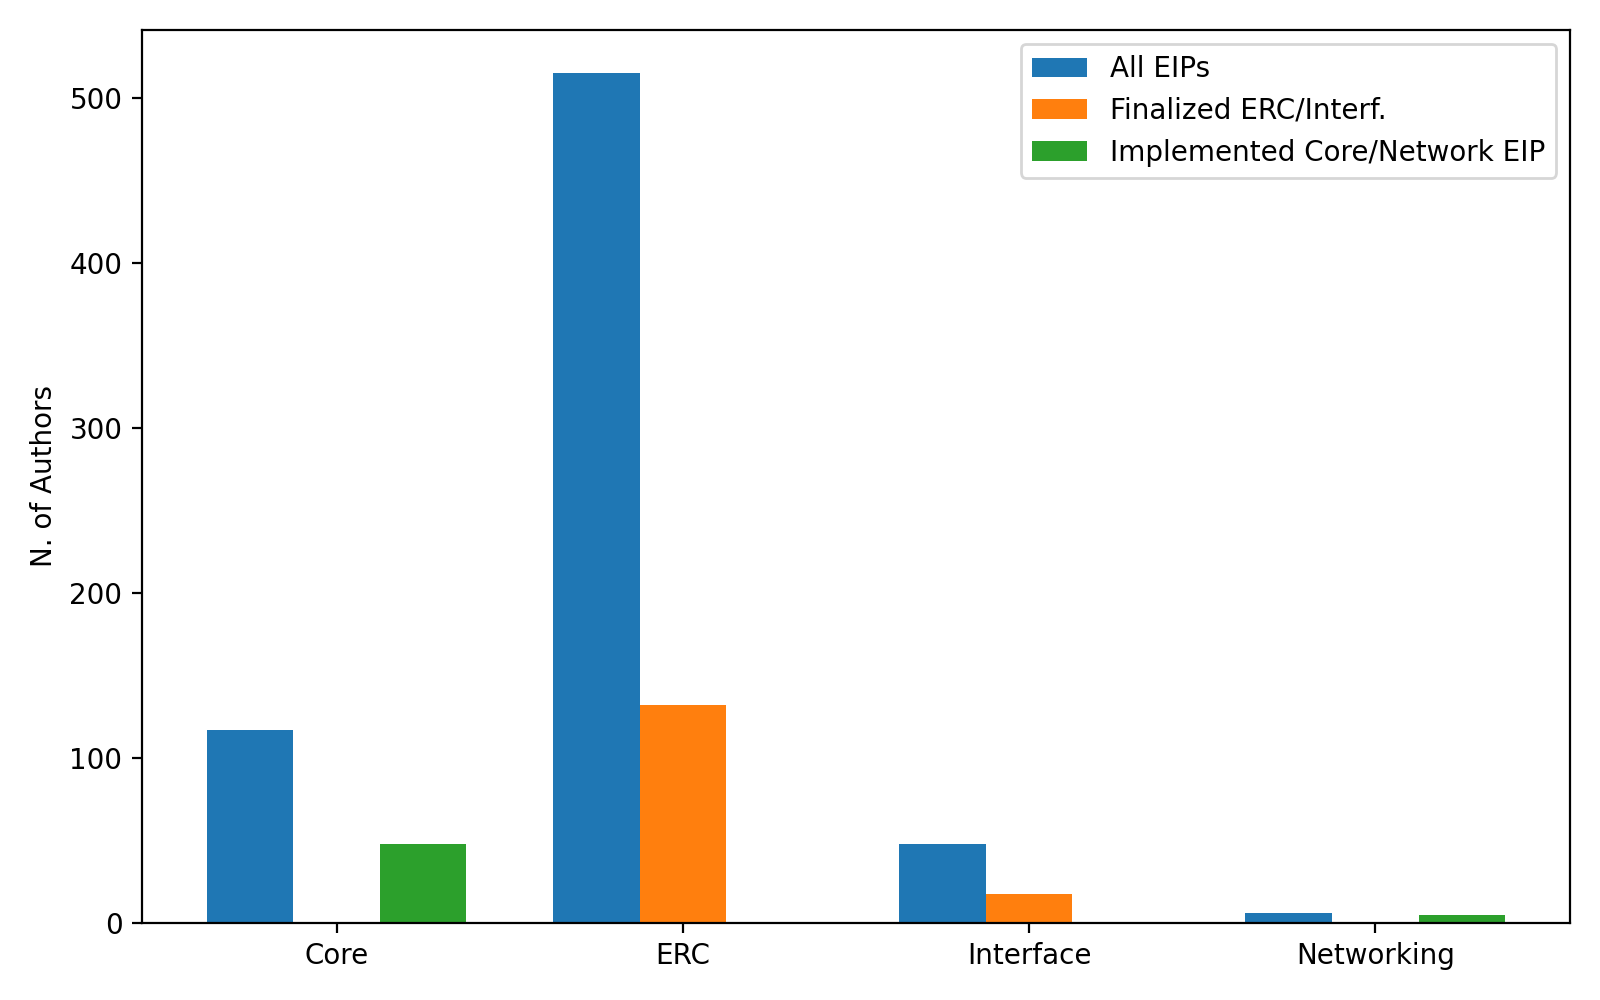
\includegraphics[width = 0.8\textwidth]{Figures/n_authors_by_stage.png}}
    \label{n_author_by_stage}
\end{figure}
%%%%%%%%%%%%%%%%%%%%%%%%%%%%%%%%%%%%%%%%%%%%%%%%%%%%%%%

We then shift focus to the disparity in contributions among authors. A few authors are exceptionally prolific, with figure \ref{top10_author} illustrating the top 10 EIP contributors across different EIP categories. Vitalik Buterin, Ethereum's co-founder, is the most prolific proposer of EIPs. However, when we focus on EIPs that have actually been approved, we find that authors seem to specialize their contributions either on Core or ERC EIPs: None of the top 10 ERC EIP authors are in the top 10 of Core EIPs. 

%%%%%%%%%%%%%%%%%%%%%%%%%%%%%%%%%%%%%%%%%%%%%%%%%%%%%%%
\begin{figure}[ht!]
    \caption{Top 10 EIP Authors}
     \begin{small}
    \begin{minipage}{\textwidth}
      This figure shows the top 10 authors ranked in terms of how many EIPs they co-authored. The top figure includes all EIPs, whether they have been approved or not. The figure on the lower left only focuses on authorship of finalized ERC/Interf EIPs. The figure on the lower right focuses on authorship of Implemented Core/Network EIPs.    
     \end{minipage}
         \end{small}
         \\[0.5cm]
    \makebox[\textwidth][c]{\begin{tabular}{cc}
    \hspace{5cm} All EIPs  \\
     \multicolumn{2}{c}{ 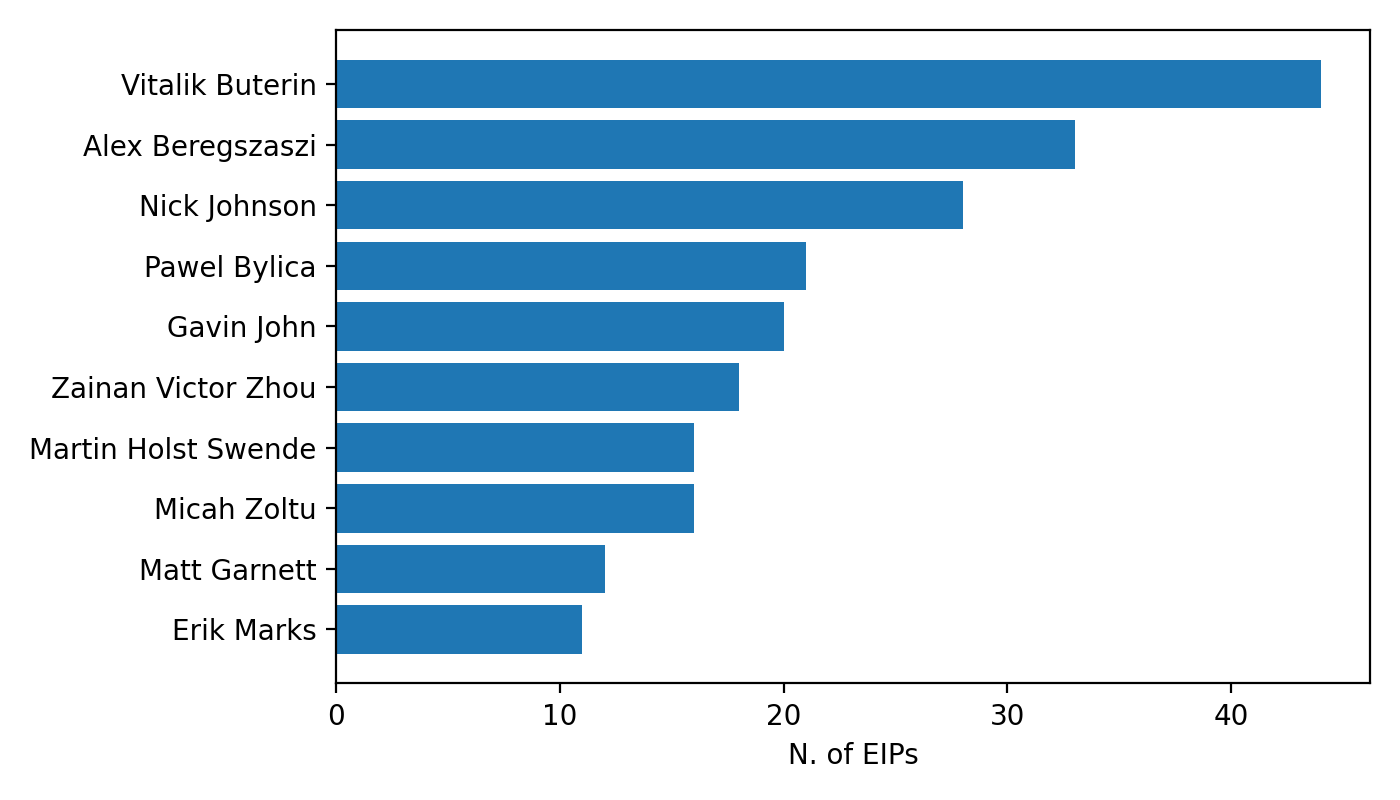
\includegraphics[width =.55\textwidth]{Figures/neip_top10author.png}} \\
      \hspace{-1cm} Finalized ERCs/Interf. &       \hspace{-1cm} Implemented Core/Network EIPs \\ \hspace{-1cm}
      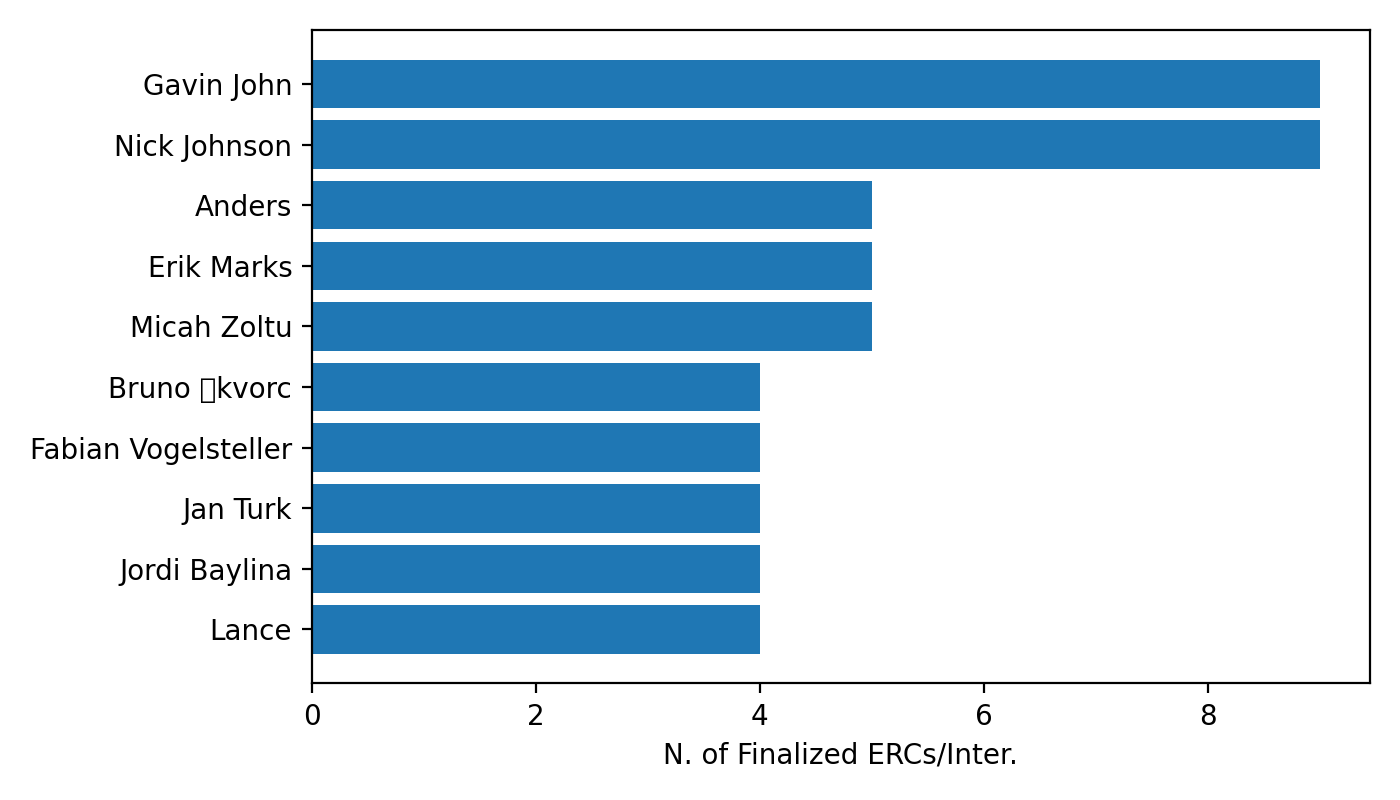
\includegraphics[width =.55\textwidth]{Figures/neip_final_top10author.png}   &
      \hspace{-1cm}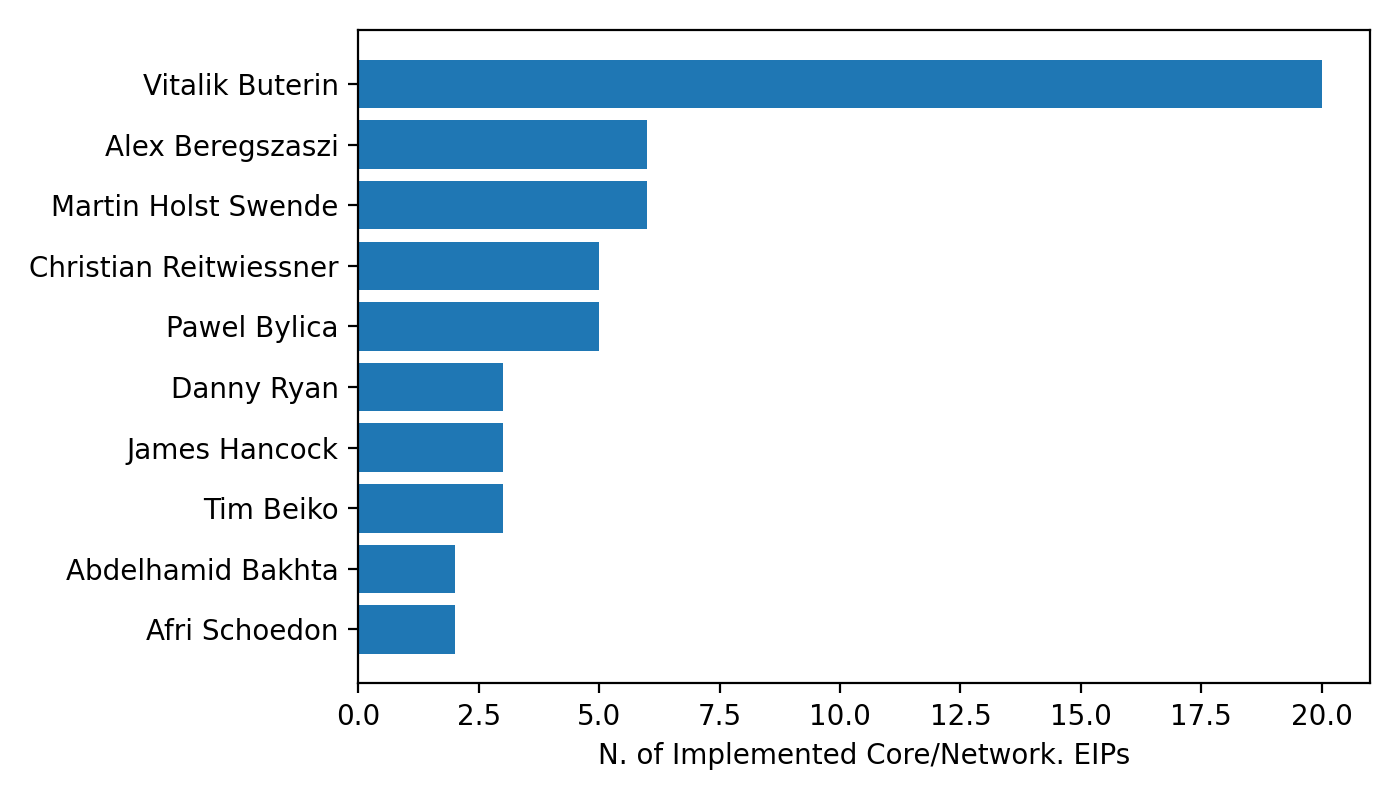
\includegraphics[width =.55\textwidth]{Figures/neip_imp_top10author.png}   \\
    \end{tabular} }
    \label{top10_author}
\end{figure}

We can also use network analysis to explore which authors are more centrally located in the EIP co-authorship network. We create an undirected weighted graph where each node is an EIP author, and each node pair is connected with a weight proportional to the number of times the two individuals co-author an EIP together. Figure \ref{fig:between} depicts the network's spring layout, revealing cliques around prolific authors like Gavin John, Vitalik Buterin, Nick Johnson, Fabian Vogelsteller, and Charles Cooper, emphasizing their central role in the EIP production. 

%%%%%%%%%%%%%%%%%%%%%%%%%%%%%%%%%%%%%%%%%%%%%%%%%%%%%%%
\begin{figure}[h!]
    \caption{EIP Co-Authorship Network}
     \begin{small}
    \begin{minipage}{\textwidth}
      This figure shows the EIP co-authorship network, restricted to the largest connected component (251 of 685 authors; the remaining 434 authors have no or very few co-authorship ties and are not shown). Each node identifies an EIP author. Authors are connected with each other if they are co-authors in an EIP. Connections are weighted by the numbers of EIPs co-authored together. Nodes in the graph are positioned using the Fruchterman-Reingold force-directed algorithm, with attraction between nodes weighted by the number of EIPs co-authored. Node color indicates community membership, identified via greedy modularity maximization on the weighted co-authorship network (12 communities). The size of each node is proportional to its betweenness centrality value. We display the names of the top 5 percent of authors, ranked by betweenness centrality.
     \end{minipage}
     \end{small}
     \makebox[\textwidth][c]{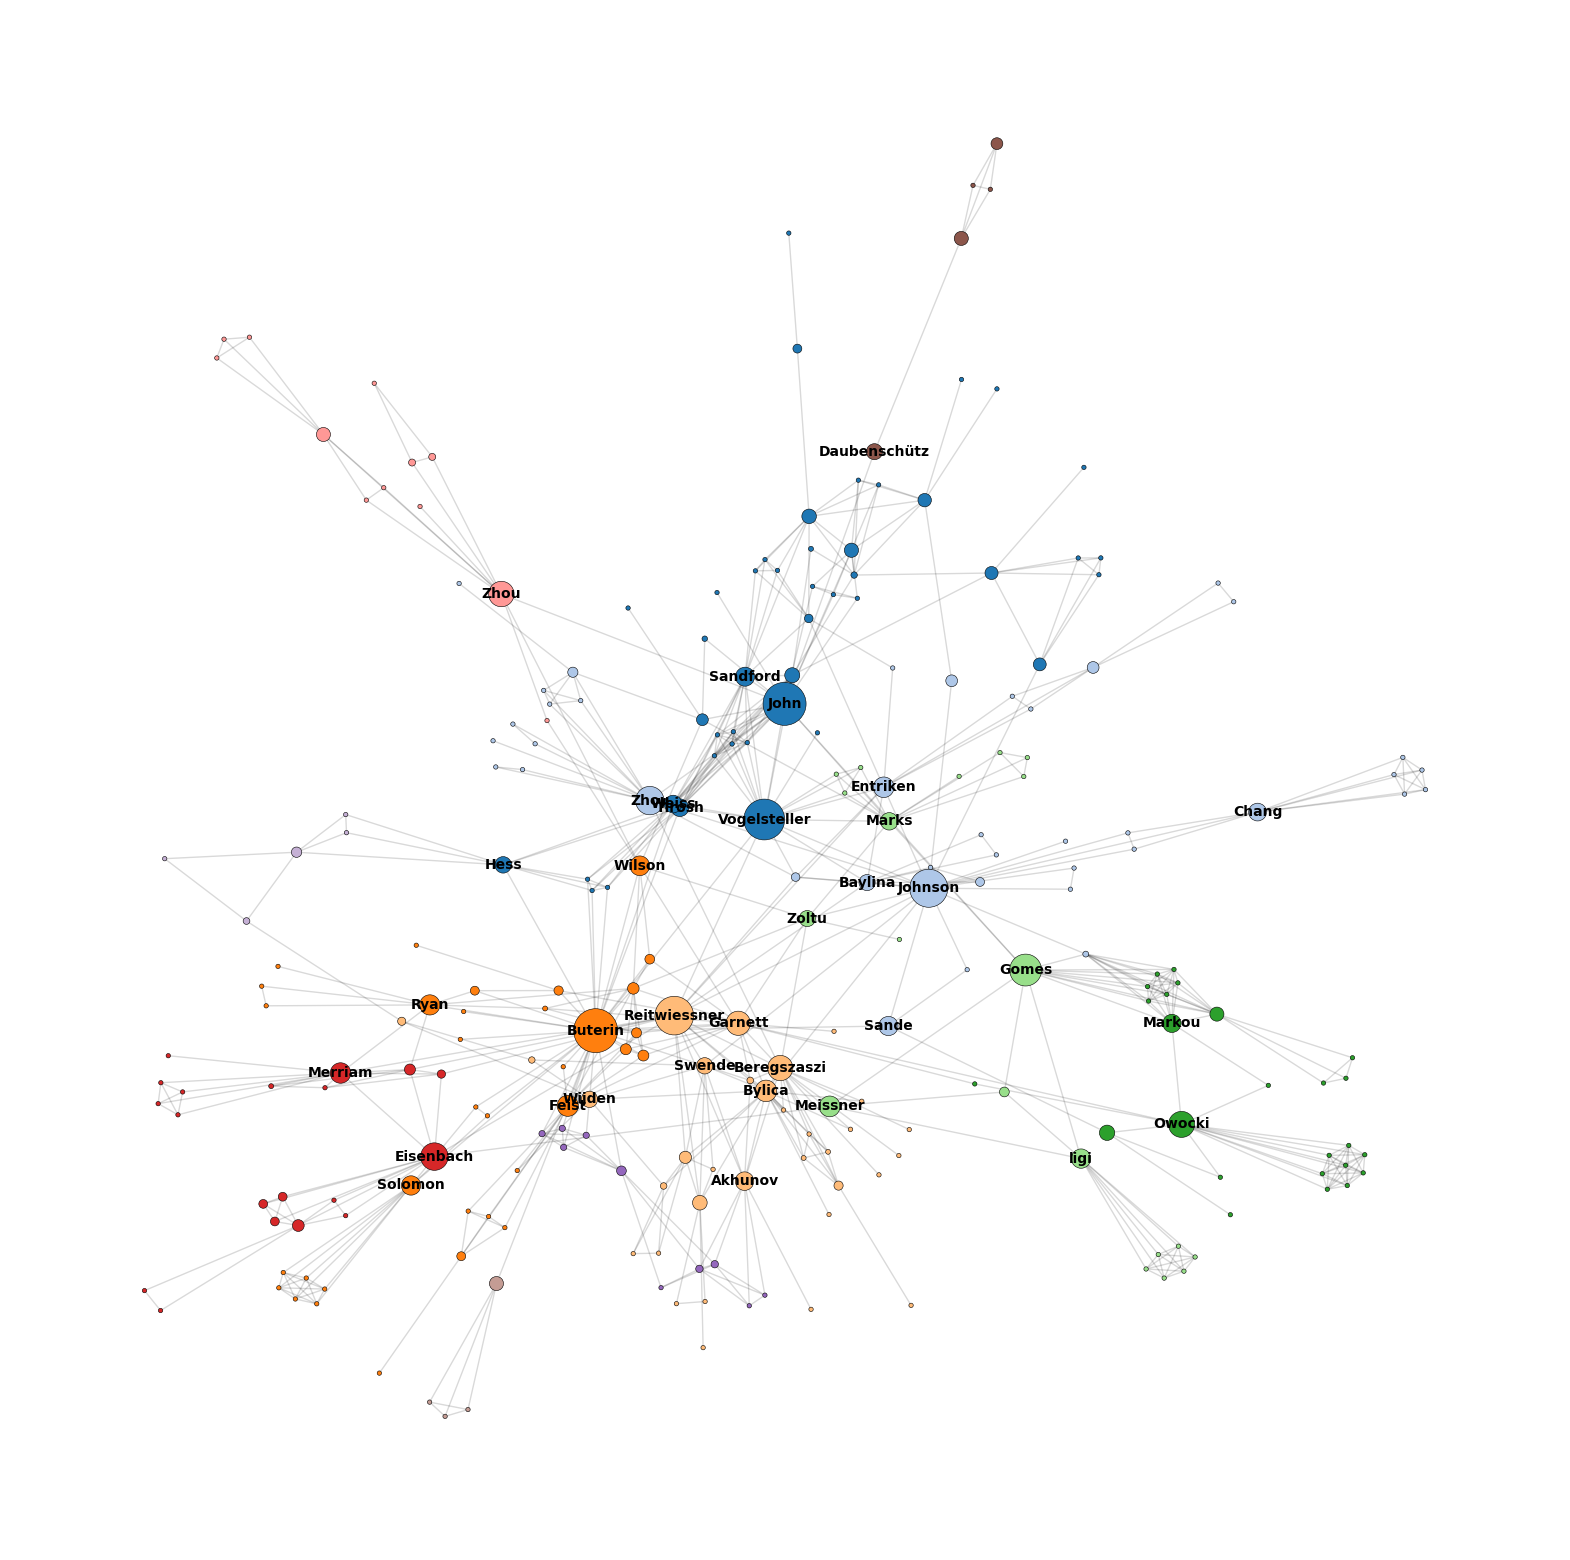
\includegraphics[width = \textwidth]{Figures/eip_between_all.png}}
     \label{fig:between}
\end{figure}


To analyze numerically the concentration of EIP production, we can use the Lorenz curve adapted to EIP authorship, as shown in Figure \ref{lorenz_authorship}, which plots the proportion of all EIPs cumulatively authored by the fraction of the population of authors in the horizontal axis. The vertical axis is the cumulative percentage of EIPs, and the horizontal axis is the number (panel a) or percentile (panel b) of authors sorted from the most to the least prolific. The top 10 EIP authors produced about 22\% of all EIPs, 31\% of finalized ERC/Interface EIPs, and 62\% of implemented Core/Networking EIPs. The Gini coefficient, defined as two times the area between the 45-degree line and the Lorenz curve in the bottom graph of Figure \ref{lorenz_authorship} \citep{Dorfman1979}, is a typical measure of concentration. The Gini coefficient for all EIPs is 0.59, but it is lower for finalized ERCs and Interface EIPs, at 0.50, and similarly high for Implemented Core/Networking EIPs, at 0.59. This is consistent with the argument that proposing Core/Networking EIPs is a much more sophisticated and time-consuming process which is the domain of few skilled individuals, while proposing ERCs and Interface EIPs is technically accessible to a wider audience.  

%%%%%%%%%%%%%%%%%%%%%%%%%%%%%%%%%%%%%%%%%%%%%%%%%%%%%%%
\begin{figure}[ht!]
    \caption{EIP Introduction Concentration}
     \begin{small}
    \begin{minipage}{\textwidth}
      This figure shows the Lorenz curve adapted to EIP authorship. The horizontal axis represents the number of authors, sorted from the most prolific to the least ones. The vertical axis represents the cumulative number of EIPs authored by the number of authors indicated in the horizontal axis. Each author is assigned a fraction of the EIP relative to the total number of co-authors on the EIP.   
     \end{minipage}
         \end{small}
         \\[0.5cm]
   \begin{subfigure}{0.49\textwidth}
           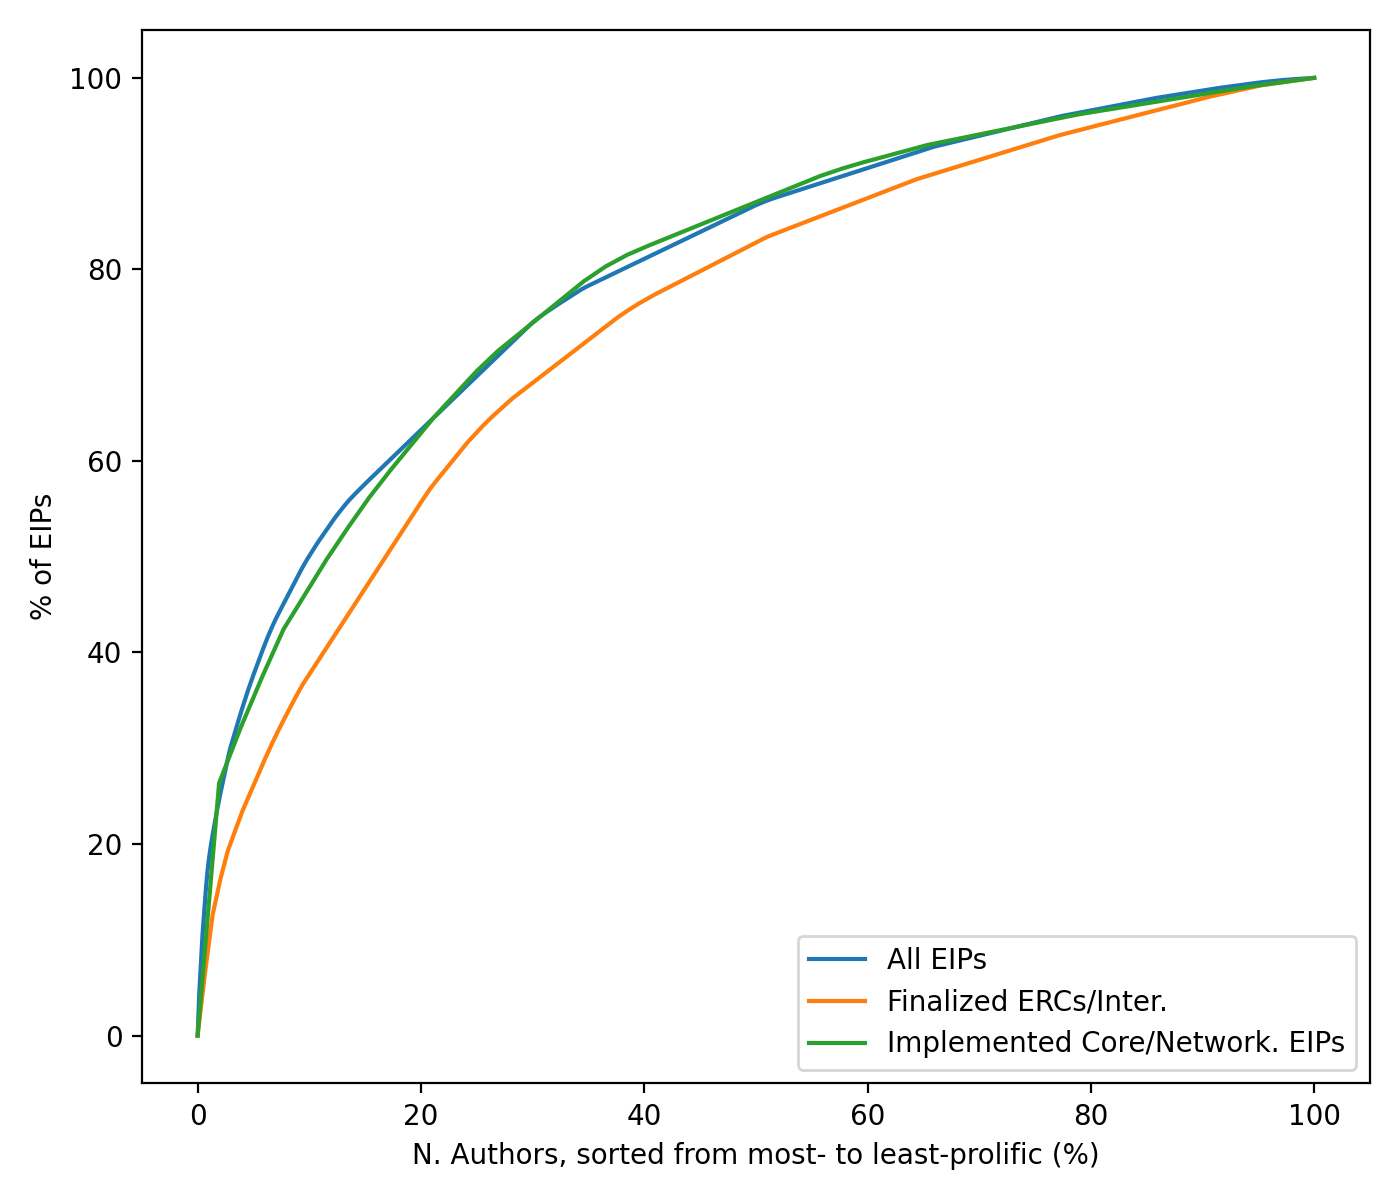
\includegraphics[width = 1\textwidth]{Figures/neip_by_author.png}
            \caption{by Number of Authors}
            \label{fig:neip}
   \end{subfigure}
    \begin{subfigure}{0.49\textwidth}
           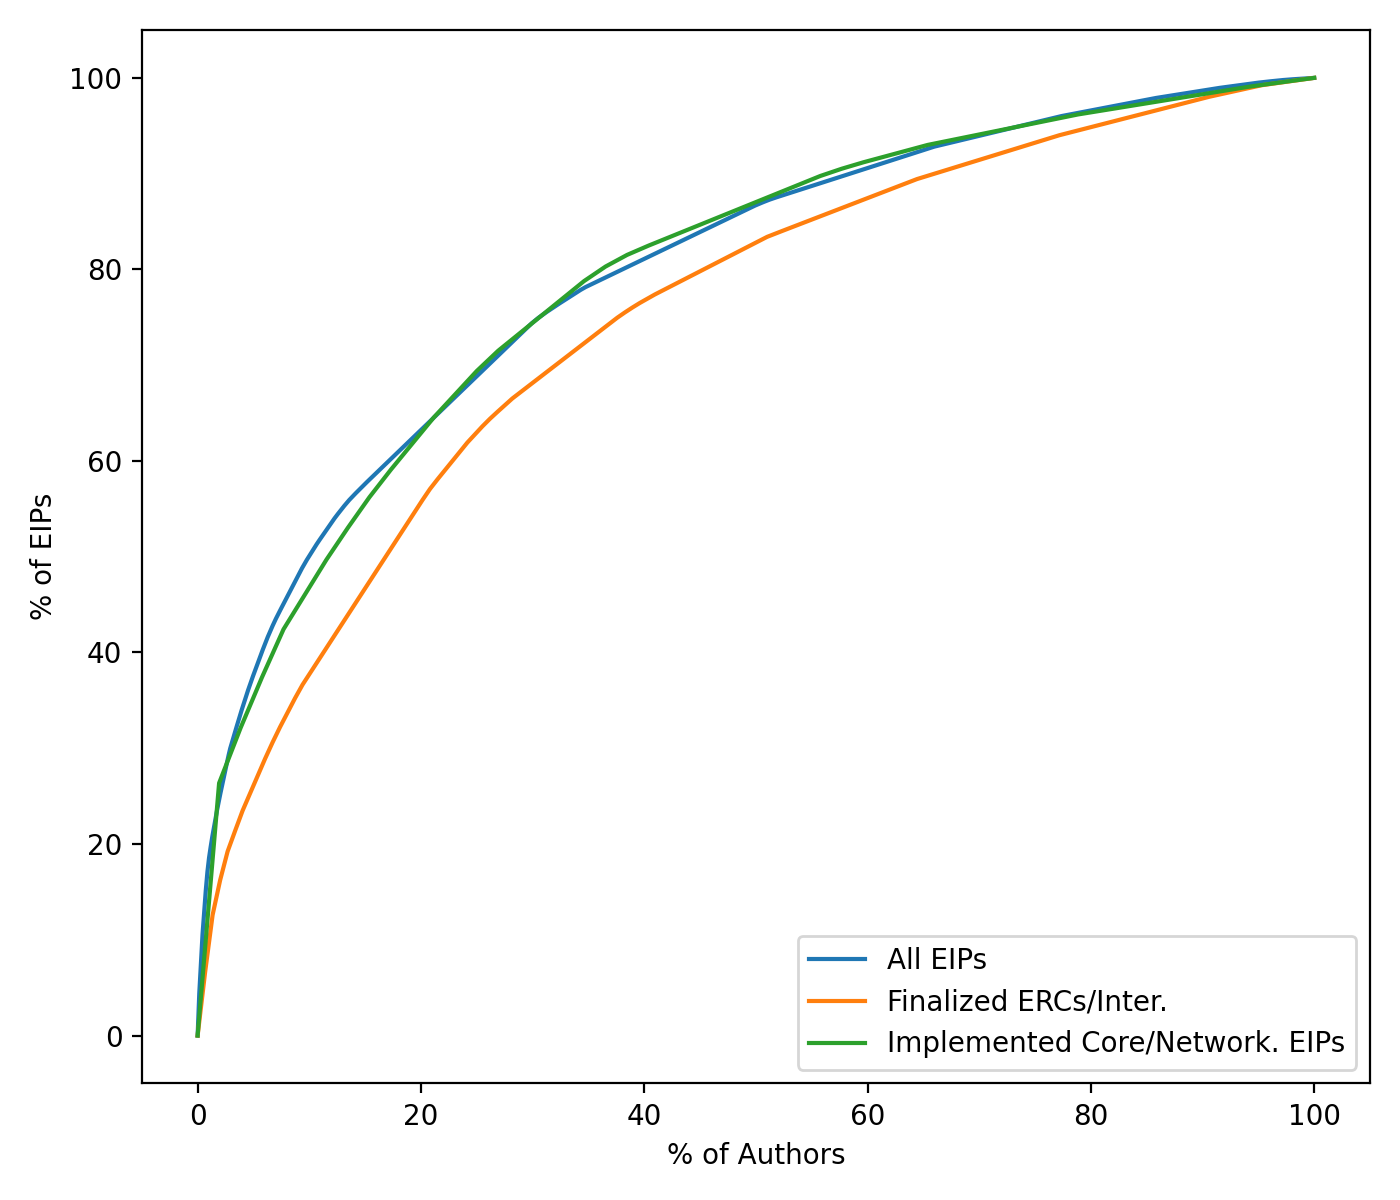
\includegraphics[width = 1\textwidth]{Figures/npeip_by_author.png}
            \caption{by Percentile of Authors}
            \label{fig:npeip}
   \end{subfigure}
  
    \label{lorenz_authorship}
\end{figure}


Our analysis covers the period from Ethereum's launch in 2015 to mid-2023. During this time, Ethereum has undergone several changes, including the expansion of its features, a shift in its core consensus mechanism, and a broadening of its community. As a result, current centralization trends in Ethereum may differ from the average outcomes observed over the entire period. We therefore examine temporal trends in decision-making concentration within Ethereum.

Given the increasing involvement in EIP authorship shown in figure \ref{fig:neip_year}, we investigate if this wider participation has led to a decreased concentration in decision-making within Ethereum's governance. To smooth out annual fluctuations in EIP production and to take into account that EIPs often take longer than one year to be implemented, we employ a two-year rolling window for our analysis. First, we examine the Gini coefficient of EIP authorship concentration. More authors do not automatically imply a lower Gini coefficient, as it could increase if new authors contribute fewer EIPs, steepening the Lorenz curve and raising the Gini coefficient. Figure \ref{fig:gini_year} shows a sharp drop in concentration around 2018-2019, but a stabilization thereafter.

%%%%%%%%%%%%%%%%%%%%%%%%%%%%%%%%%%%%%%%%%%%%%%%%%%%%%%%
\begin{figure}
    \caption{Concentration of EIP Production over Time}
     \begin{small}
    \begin{minipage}{\textwidth}
      This figure shows the Gini coefficient for each two-year rolling window. Year 2023 numbers are incomplete, as data collection ended on June 21, and are marked with an asterisk.
  \end{minipage}
         \end{small}
    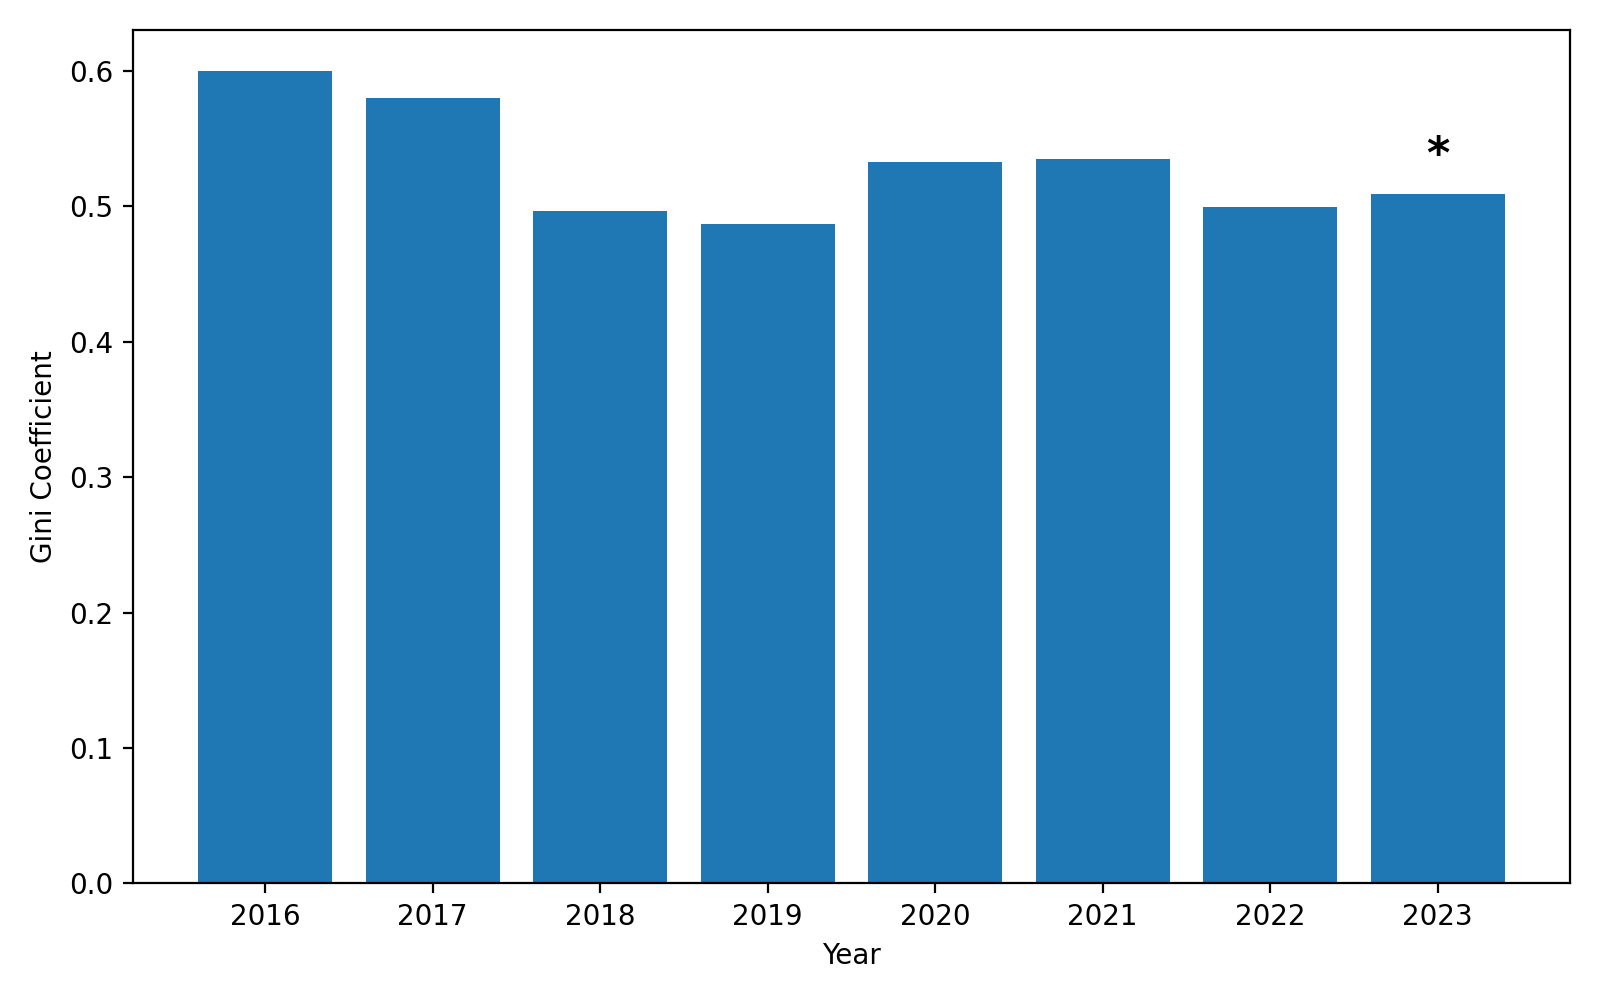
\includegraphics[width = 0.8\textwidth]{Figures/gini_by_year.png}
    \label{fig:gini_year}
\end{figure}


Finally, we can assess the decentralization of the co-authorship network measuring the average clustering coefficient, a metric used in network analysis to gauge the density of a network. More precisely, the local clustering coefficient $C_i$ for each node $i$ counts the fraction of closed triangles over the total possible triangles involving node $i$. The average clustering coefficient $C$ is the average of the individual clustering coefficients across all $n$ nodes in the network. 

\begin{equation}
    C = \frac{1}{n} \sum_i C_i = \frac{1}{n} \sum_i \frac{\sum_{j,k} A_{i,j}A_{j,k}A_{k,i}}{\sum_j A_{i,j} ( \sum_j A_{i,j} - 1)}
\end{equation} \label{eq:cc}

where $A$ is the adjacency matrix of the co-authorship network.

A network with $C=0$ is a hub-and-spoke network where there is one single central node that is connected with all other nodes, which can be thought as a very centralized network. A network with $C=1$ is a fully connected network, where all nodes have equal influence, and thus fully decentralized.

Our analysis of the co-authorship network in Figure \ref{fig:between} shows an average clustering coefficient of 0.6 over the period. The red column in Figure \ref{fig:clustering_trends} shows an upward trend from 0.5 in 2016 to over 0.65 in 2023. Such a rise in connectedness could be attributed to two main factors: The number of co-authors in each EIPs might be rising over time, or authors might be working with different people across EIPs. The blue column in the figure shows that the average number of co-authors working for an EIP has been relatively flat over the last five years, suggesting growing interconnectedness and decentralization in EIP co-authorship.


%%%%%%%%%%%%%%%%%%%%%%%%%%%%%%%%%%%%%%%%%%%%%%%%%%%%%%%
\begin{figure}[ht!]
    \caption{Decentralization of EIP Co-Authorship over Time}
     \begin{small}
    \begin{minipage}{\textwidth}
      This figure shows the clustering coefficient of the EIP co-authorship network for each two-year rolling window. The clustering coefficient is defined in eq (\ref{eq:cc}). Year 2023 numbers are incomplete, as data collection ended on June 21, and are marked with an asterisk.
  \end{minipage}
         \end{small}
            \\[0.5cm]
 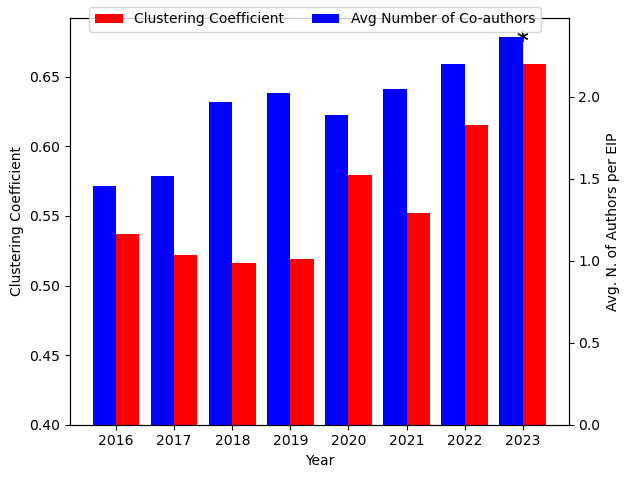
\includegraphics[width = 0.8\textwidth]{Figures/clustering_trends.png}
    \label{fig:clustering_trends}
\end{figure}

Overall, we find that the EIP production is rather concentrated in the hands of few individuals, especially for the most important EIPs which introduce a change to the protocol. Such concentration has remained relatively constant over the last 5 years. We also find that a handful of authors are in the center of the co-authorship network, even though lately the network has become more decentralized. Next we turn to how these proposals are discussed and approved in the Ethereum community. 


%%%%%%%%%%%%%%%%%%%%%%%%%%%%%%%%%%%%%%%%%%%%%%%%%%%%%%%%%%%%%%%%
\subsection{Concentration in EIP Discussion} \label{subsec:concentration_EIP_Discussion}
%%%%%%%%%%%%%%%%%%%%%%%%%%%%%%%%%%%%%%%%%%%%%%%%%%%%%%%%%%%%%%%%

As explained above, three main open venues are used to discuss EIPs: the Fellowship of Ethereum Magicians (FEM) forum, github repositories, and the AllCoreDevs calls. 

We begin by analyzing the participation and concentration of discussions in the FEM forum. on the forum, each EIP is allocated a discussion board. This platform allows anyone to pose questions or suggest amendments to the proposal. We are able to find 448 EIPs discussed on the board.\footnote{FEM was launched only on Feb 16, 2018, thus the early EIPs did not have a formal venue for discussion.} So far, 1,370 unique individuals have contributed to these discussions, resulting in 3.4M views, 9,271 comments, and 7,129 likes. Panel (a) of table \ref{tab:participation_summary} shows that on average, 5 unique participants actively commented for each poposals, with 5,573 views and 15 comments. Panel (a) of Figure \ref{fig:FEM} shows that the community engagement has been increasing over time, with views growing at a compound annual rate of about 13\% from 2018 to 2022. Contributors are not all equally engaged with the discussion, as shown in the Lorenz Curve in panel (b) of Figure \ref{fig:FEM}. The top 10 FEM contributors account for 23.3\% of all comments, with a moderately high Gini coefficient of 72.6\%.


%%%%%%%%%%%%%%%%%%%%%%%%%%%%%%%%%%%%%%%%%%%%%%%%%%%%%%%
\begin{table}[ht!]
    \caption{Participation in EIP Discussion by Venue}
     \begin{small}
    \begin{minipage}{\textwidth}
      This table reports summary statistics of EIP discussion and development activity across three venues: the Fellowship of Ethereum Magicians forum (Panel A), GitHub (Panel B), and AllCoreDevs calls (Panel C). FEM Comments/Views/Likes are totals for the EIP's forum thread, and Active Participants is the number of unique commenters. GitHub Commits counts commits to the EIP's file in the EIPs repository; Comment and Reviews count, respectively, general pull-request/issue comments and formal review submissions (including inline review comments) on the EIP. Panel C is computed per AllCoreDevs call rather than per EIP: Active Participants per Meeting is the number of unique attendees at a given call, over all calls from 2015 onward.
  \end{minipage}
         \end{small}
    \makebox[\textwidth][c]{\begin{tabular}{lrrrrr}
\toprule
 & Mean & Median & Std. Dev. & Min & Max \\
\midrule
\multicolumn{6}{l}{\textbf{Panel A. Fellowship of Ethereum Magicians (FEM)}} \\
Comments & 15.15 & 5.00 & 33.00 & 0.00 & 476.00 \\
Views & 5573.35 & 2861.00 & 11935.59 & 0.00 & 166037.00 \\
Likes & 11.65 & 2.00 & 32.57 & 0.00 & 443.00 \\
Active Participants & 5.16 & 3.00 & 8.91 & 0.00 & 108.00 \\
\midrule
\multicolumn{6}{l}{\textbf{Panel B. GitHub}} \\
Commits & 6.66 & 5.00 & 6.21 & 0.00 & 30.00 \\
Comment & 14.26 & 4.00 & 48.81 & 0.00 & 708.00 \\
Reviews & 17.96 & 11.00 & 23.58 & 0.00 & 181.00 \\
\midrule
\multicolumn{6}{l}{\textbf{Panel C. AllCoreDevs}} \\
Active Participants per Meeting & 20.82 & 19.00 & 7.20 & 4.00 & 38.00 \\
\bottomrule
\end{tabular}
}
    \label{tab:participation_summary}
\end{table}
%%%%%%%%%%%%%%%%%%%%%%%%%%%%%%%%%%%%%%%%%%%%%%%%%%%%%%%



%%%%%%%%%%%%%%%%%%%%%%%%%%%%%%%%%%%%%%%%%%%%%%%%%%%%%%%
\begin{figure}[ht!]
    \caption{Discussion on Fellowship of Ethereum Magicians}
     \begin{small}
    \begin{minipage}{\textwidth}
      Panel (a) shows the number of views received ordered by year in which the EIP discussion was initiated on the Fellowship of Ethereum magicians (FEM) discussion board. Year 2023 is incomplete, as data collection stopped in June 2023, and is marked with an asterisk. Panel (b) shows the Lorenz curve for comments on the discussion board by contributor. The vertical axis is the percentage of all comments made by the most prolific contributors, and the horizontal axis is the number of contributors sorted by the most to the least prolific. 
 
     \end{minipage}
         \end{small}
         \\[0.5cm]
   \begin{subfigure}{0.49\textwidth}
           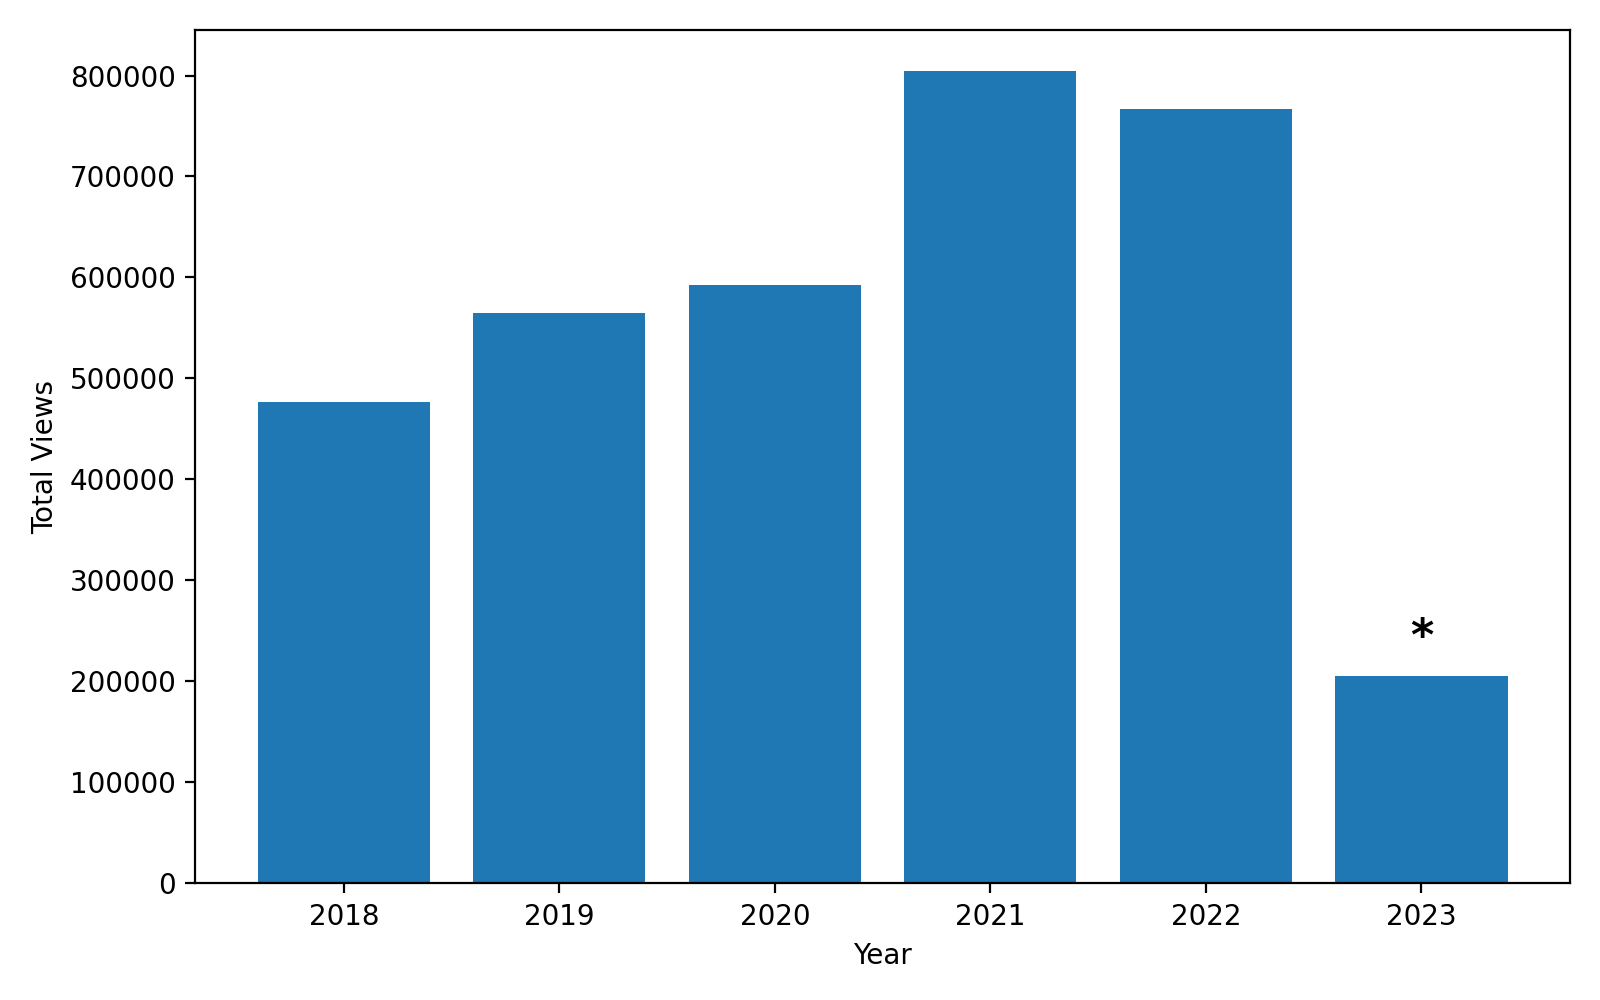
\includegraphics[width = 1\textwidth]{Figures/FEM_Views_year.png}
            \caption{FEM Views by EIP Year}
            \label{fig:FEM_Views_year}
   \end{subfigure}
    \begin{subfigure}{0.49\textwidth}
           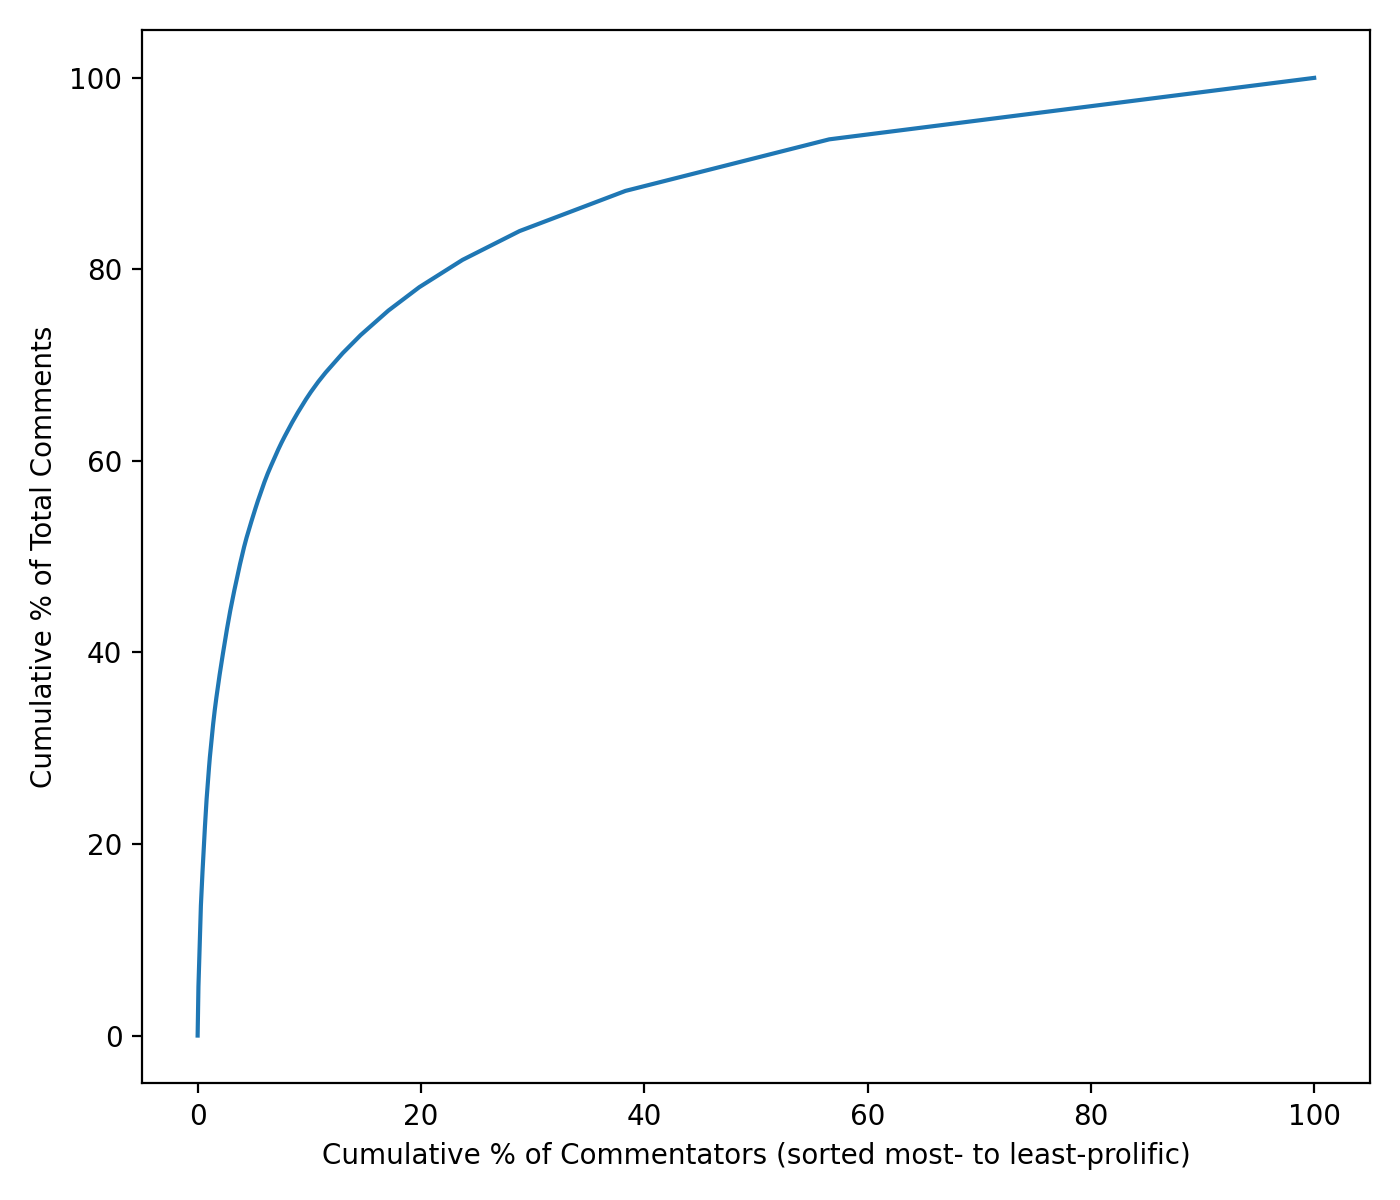
\includegraphics[width = 1\textwidth]{Figures/FEM_Lorenz_Comments.png}
            \caption{Lorenz Curve of FEM Contributors}
            \label{fig:FEM_Lorenz_Comments}
   \end{subfigure}
  
    \label{fig:FEM}
\end{figure}
%%%%%%%%%%%%%%%%%%%%%%%%%%%%%%%%%%%%%%%%%%%%%%%%%%%%%%%

We next turn to github repositories. Each EIP has a corresponding document where feedback can be directly incorporated via pull requests. Authors then have the discretion to either integrate and commit these changes into the main branch or reject them. Github also allows users to provide comments on the posted proposal, and reviewers can respond in line to the comments.

To assess the extent of meaningful contributions from participants other than the authors, we downloaded all GitHub commits, comments, and reviews for each EIP. Panel B of table \ref{tab:participation_summary} shows that on average there are nearly 7 commits per EIP. Figure \ref{fig:commit_total} differentiates between commits made by authors and those by external contributors, excluding bot-generated commits, with 85\% originating from authors and only 15\% from external contributors. A small subset of EIPs have received over 30 commits. 

%%%%%%%%%%%%%%%%%%%%%%%%%%%%%%%%%%%%%%%%%%%%%%%%%%%%%%%
\begin{figure}
    \caption{Number of GitHub Commits by EIP}
     \begin{small}
    \begin{minipage}{\textwidth}
      This figure shows the histogram of the number of GitHub commits by EIP. The blue bar represents the fraction of commits in the bin that are made by the authors of the EIP, and the red bar by other contributors.   
  \end{minipage}
         \end{small}
    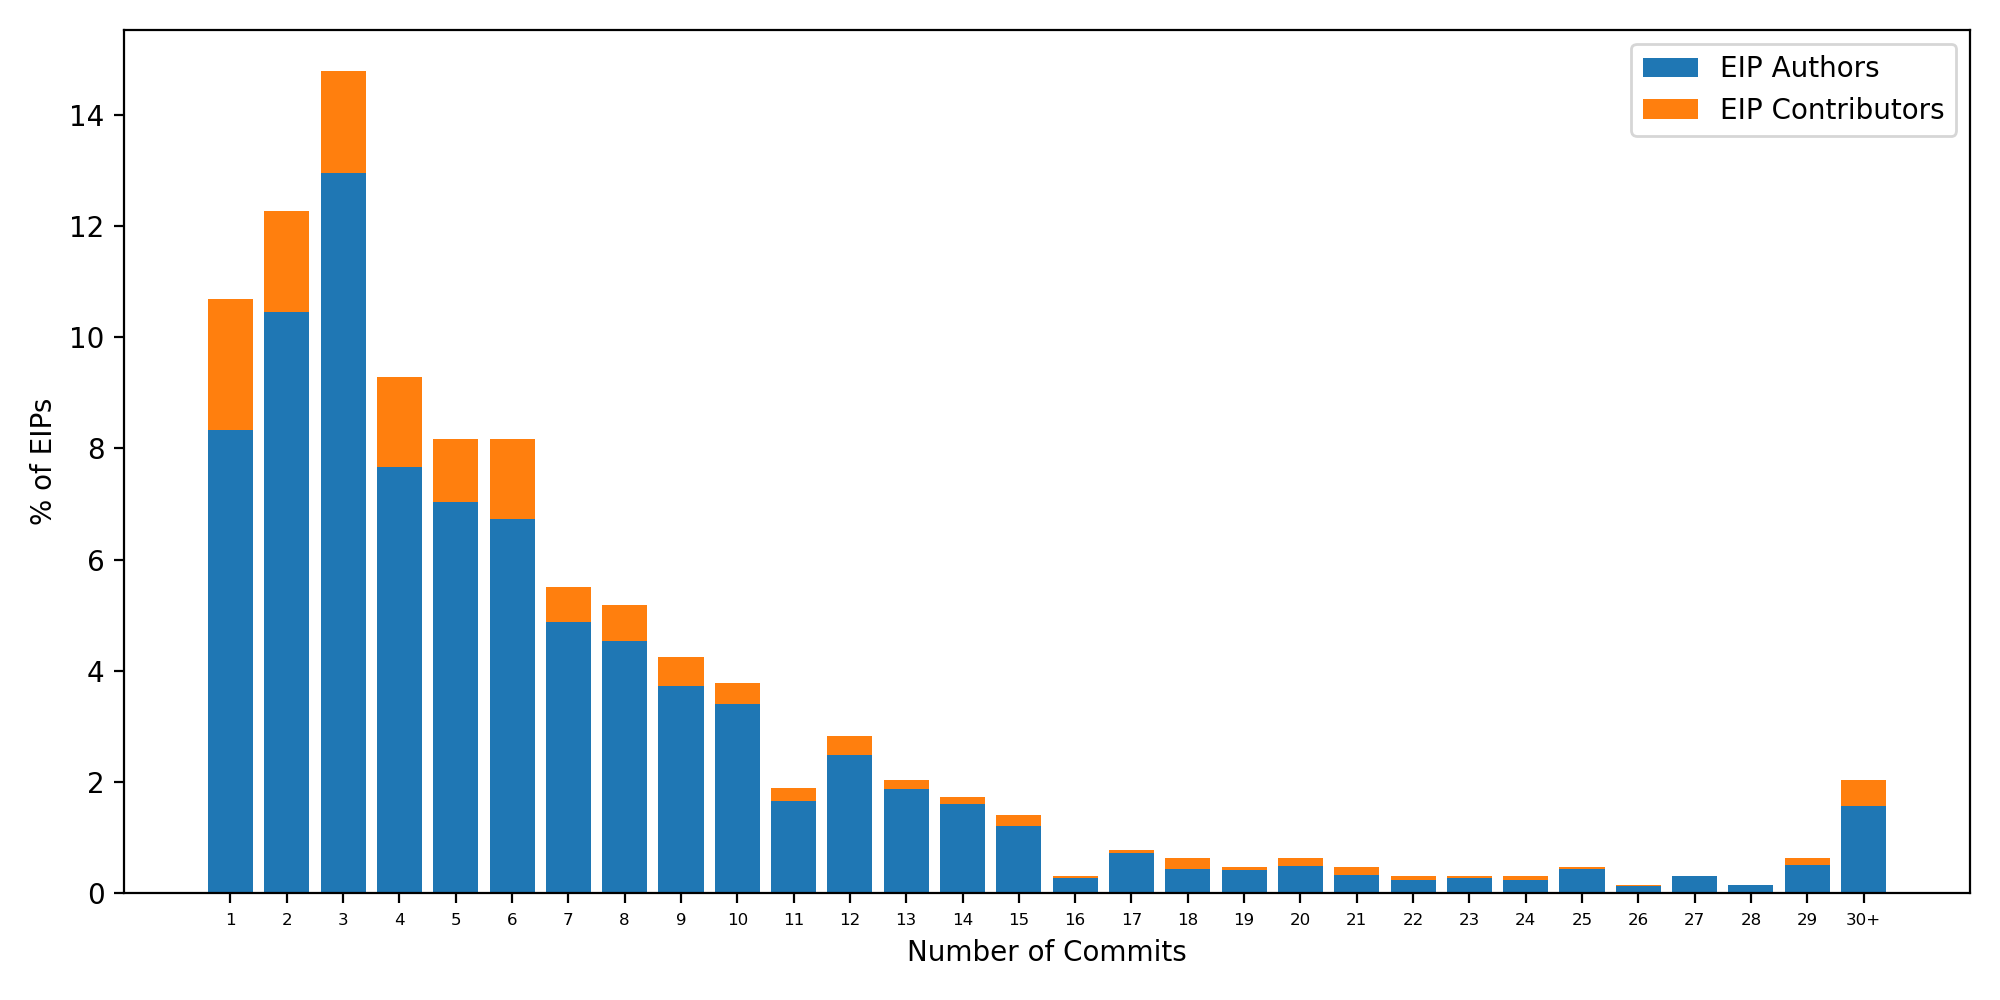
\includegraphics[width = 0.8\textwidth]{Figures/commit_total.png}\label{fig:commit_total}
\end{figure}
%%%%%%%%%%%%%%%%%%%%%%%%%%%%%%%%%%%%%%%%%%%%%%%%%%%%%%%

While changes to the proposals are mostly done by authors, each EIP receives on average 14 comments by external participants, and authors respond to most of these comments. We thus conclude that github repositories are as active as FEM in broadening the participation to governance proposals.  
















Finally, we look at AllCoreDevs calls. These live-streamed events are moderated by a facilitator, who sets the agenda and invites participants to talk. These meetings focus solely on core EIPs due to their technical nature, and the main goal is to refine and finalize EIPs for client implementation. As of June 2023, there have been 154 meetings with 387 unique attendees. As shown on panel C of table \ref{tab:participation_summary}, on average, 20 individuals actively attend each call. The number of attendees has been growing over time, from around 15 in the early years to nearly double that number by the end of our study period, as shown in figure \ref{fig:attendees_year}. 18\% of meeting attendees are EIP authors, and 20\% are client developers, while the rest come from the broader Ethereum community. Figure \ref{fig:attended_eip} shows that the most prolific EIP authors are also the most likely to attend the developers meetings. 

%%%%%%%%%%%%%%%%%%%%%%%%%%%%%%%%%%%%%%%%%%%%%%%%%%%%%%%
\begin{figure}[ht!]
    \caption{AllCoreDevs Calls Attendees}
     \begin{small}
    \begin{minipage}{\textwidth}
      Panel (a) shows the average number of attendees at the bi-weekly AllCoreDevs Calls over time. Panel (b) shows a scatter plot where each dot is an EIP author. The vertical axis measures the number of AllCoreDevs meetings attended by the author, and on the horizontal axis the number of EIPs co-authored. In panel (a), the year 2023 value is incomplete, as data collection ended on June 21, and is marked with an asterisk.

     \end{minipage}
         \end{small}
         \\[0.5cm]
   \begin{subfigure}{0.49\textwidth}
           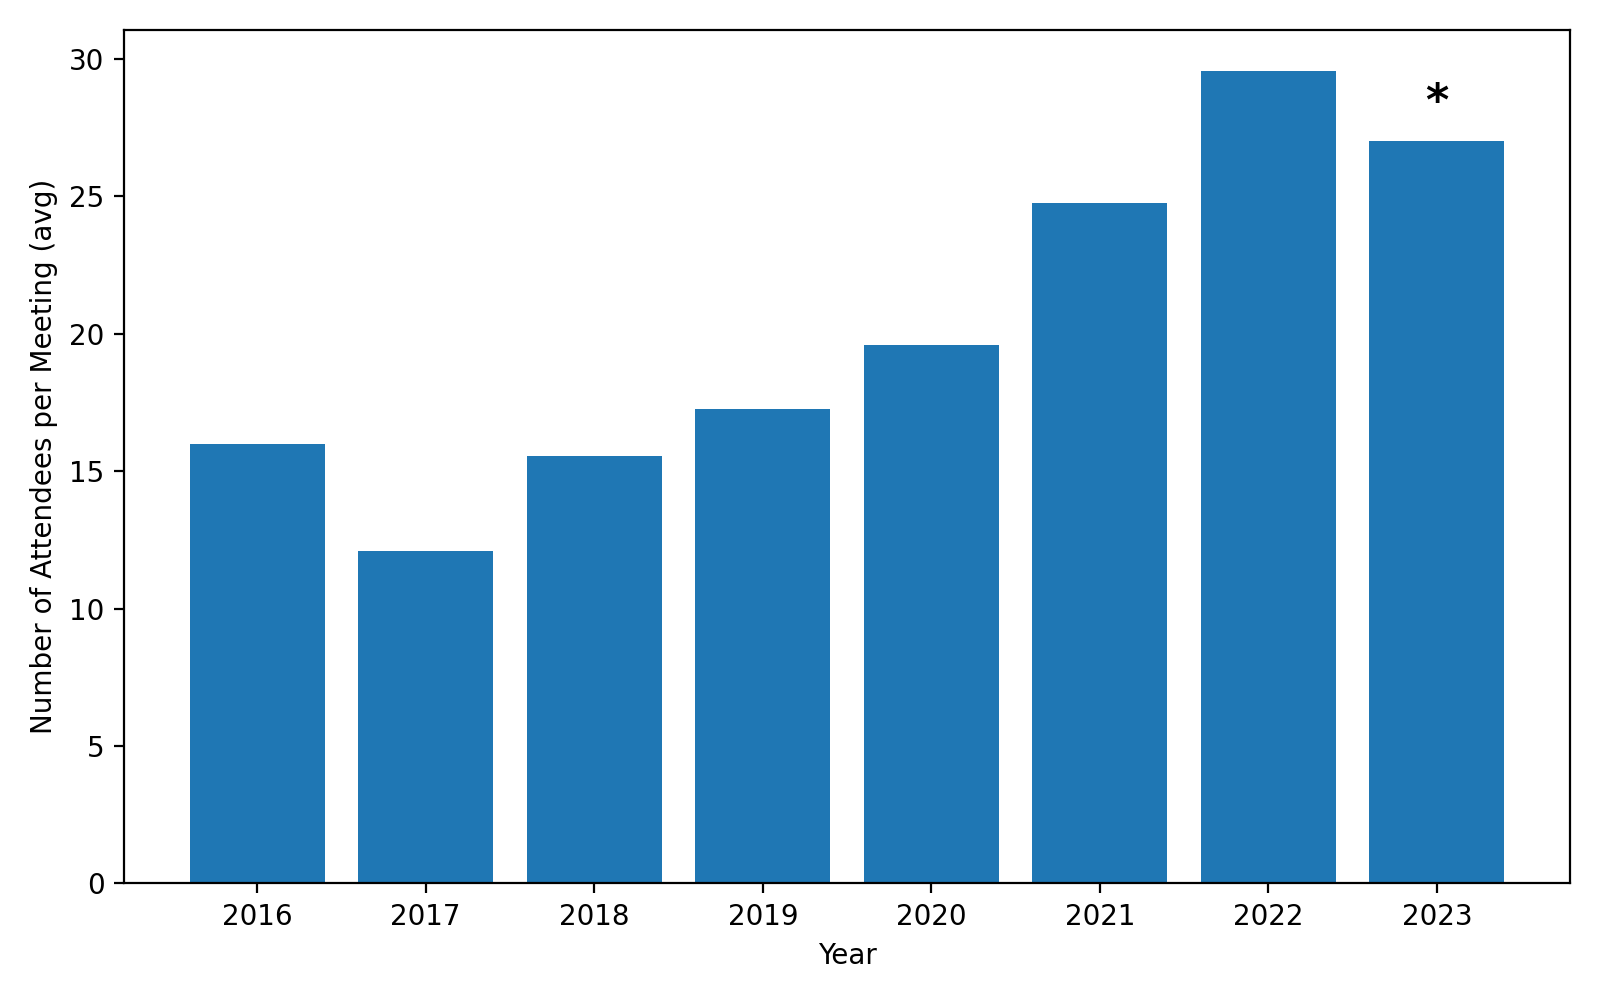
\includegraphics[width = 1\textwidth]{Figures/attendees_year.png}
            \caption{N. Attendees by Year}
            \label{fig:attendees_year}
   \end{subfigure}
    \begin{subfigure}{0.49\textwidth}
           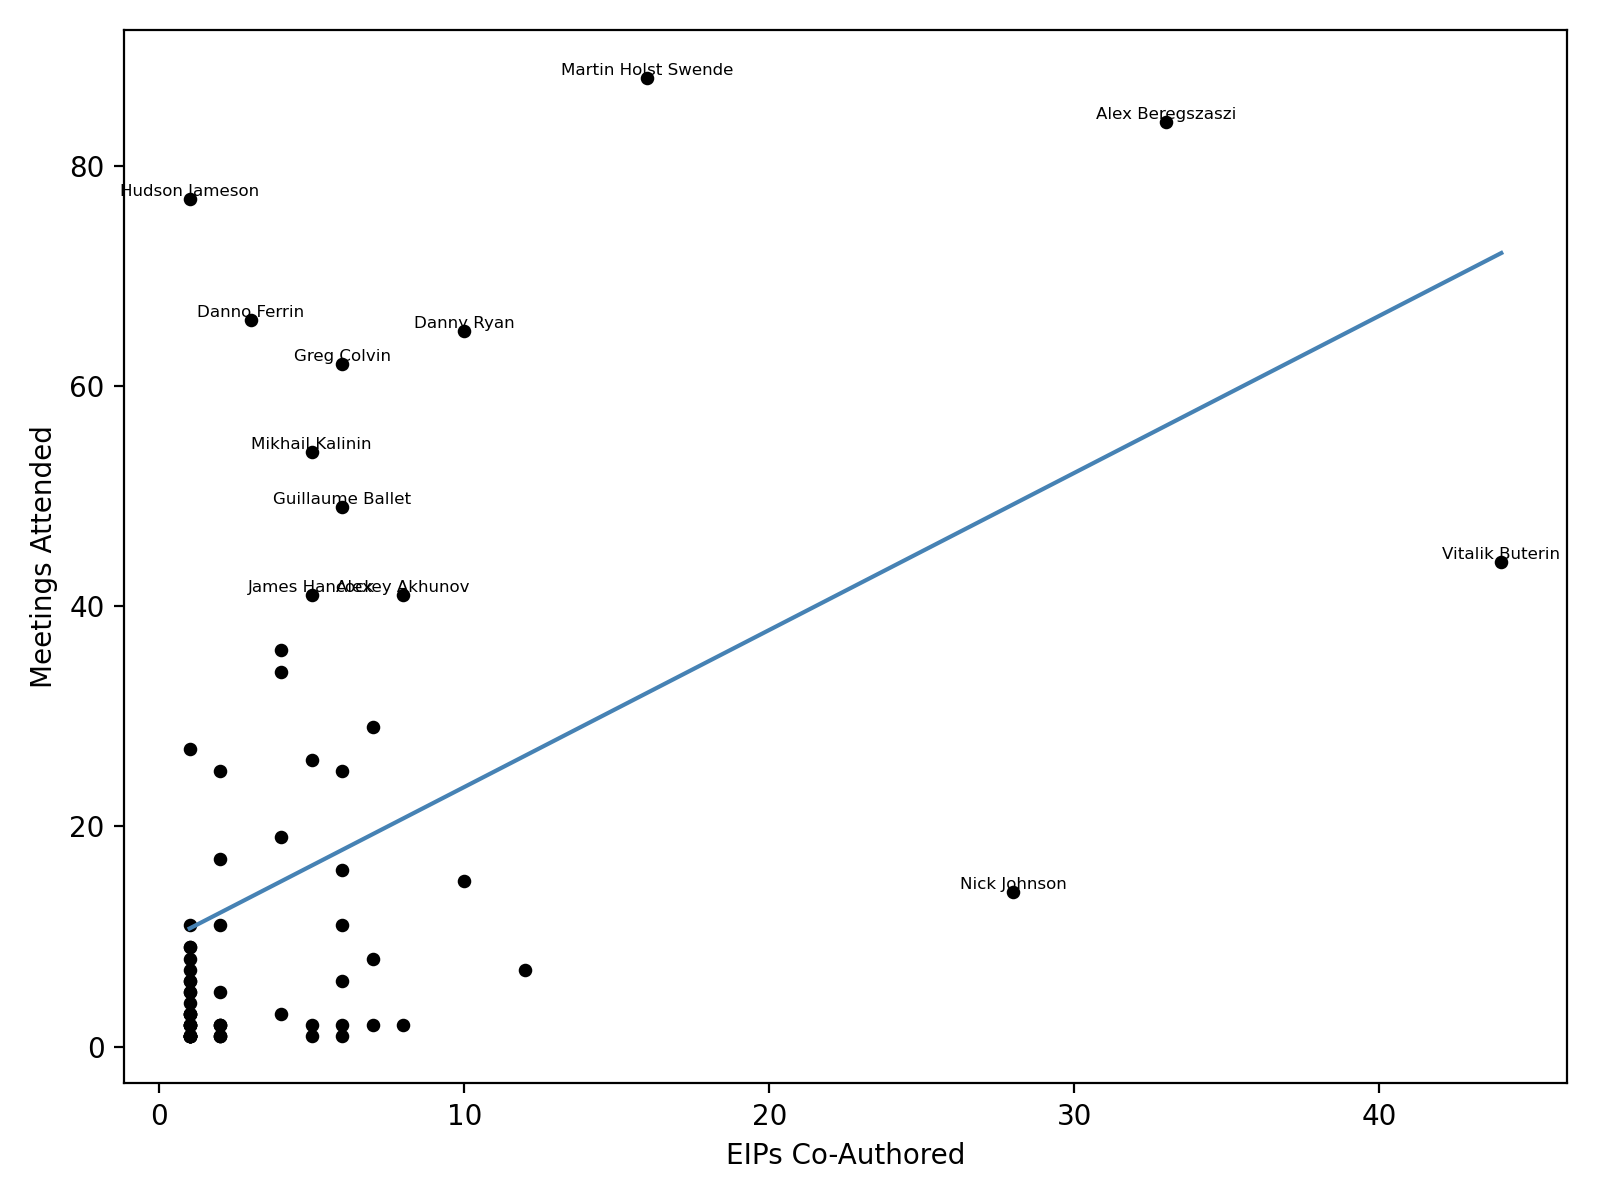
\includegraphics[width = 1\textwidth]{Figures/attended_eip.png}
            \caption{Attendees and EIP Authorship}
            \label{fig:attended_eip}
   \end{subfigure}
  
    \label{fig:attendees}
\end{figure}
%%%%%%%%%%%%%%%%%%%%%%%%%%%%%%%%%%%%%%%%%%%%%%%%%%%%%%%

In contrast with what we have uncovered on the elevated concentration in EIP proposal, the participation in the discussion of EIP is broad-based, both in the number of official venues, from FEM forum, to github repositories and AllCoreDevs meetings, as well in the number of active participants in these venues. 


%%%%%%%%%%%%%%%%%%%%%%%%%%%%%%%%%%%%%%%%%%%%%%%%%%%%%%%%%%%%%%%%
\subsection{Concentration in Client Development} \label{subsec:concentration_client_development}
%%%%%%%%%%%%%%%%%%%%%%%%%%%%%%%%%%%%%%%%%%%%%%%%%%%%%%%%%%%%%%%%


The finalization of core EIPs marks the beginning of an important phase where core client developers integrate these changes into the client software. Ethereum currently operates with four main clients: Geth, Besu, Nethermind, and Erigon. Our objective is to analyze the involvement and concentration of development efforts among these clients using GitHub commit data.

We start by aggregating all commits from the GitHub repositories of these clients. In total, around 1,277 unique contributors have made contributions, amounting to 47,400 commits. Among these, Geth emerges as the most contributed-to client with 868 unique contributors, followed by Erigon with 760, Besu with 157, and Nethermind with 106. Despite the seemingly large number of contributors, most of them contribute on a very small scale: over 80\% of the contributors have made fewer than 7 commits, accounting for about 5.5\% of the total commits. 

To further understand the concentration of client implementation efforts, we employ a similar method to that used in section \ref{subsec:concentration_EIP_Proposal}. We rank developers by the number of client commits, and then plot a Lorenz curve to represent the cumulative percentage of commits by these contributors. Figure \ref{fig:lorenz_commits} reveals a concentration of contributions in the hands of a few developers across all four main clients, with an average Gini coefficient of 89\%. Specifically, Nethermind shows the steepest Lorenz curve, with 7 developers responsible for 80\% of commits, followed by Erigon with 17 and Geth with 18 developers, whereas Besu has the least concentration with 23 developers contributing 80\% of commits. 

Client software development is clearly concentrated in the hands of very few contributors, most of whom are affiliated with the Ethereum Foundation or Consensys, as we show in section \ref{subsec:companies}. Given the critical role of client implementation in the EIP governance process, this is an area that warrants more discussion and disclosure regarding inside information and conflict of interests. 


%%%%%%%%%%%%%%%%%%%%%%%%%%%%%%%%%%%%%%%%%%%%%%%%%%%%%%%
\begin{figure}[htb!]
    \caption{Client Implementation Concentration}
     \begin{small}
    \begin{minipage}{\textwidth}
      This figure shows the Lorenz curve adapted to Client Commits Concentration. The horizontal axis represents the fraction of developers, sorted from the most prolific to the least ones. The vertical axis represents the cumulative number of commits authored by the number of developers indicated in the horizontal axis. 
  \end{minipage}
         \end{small}
    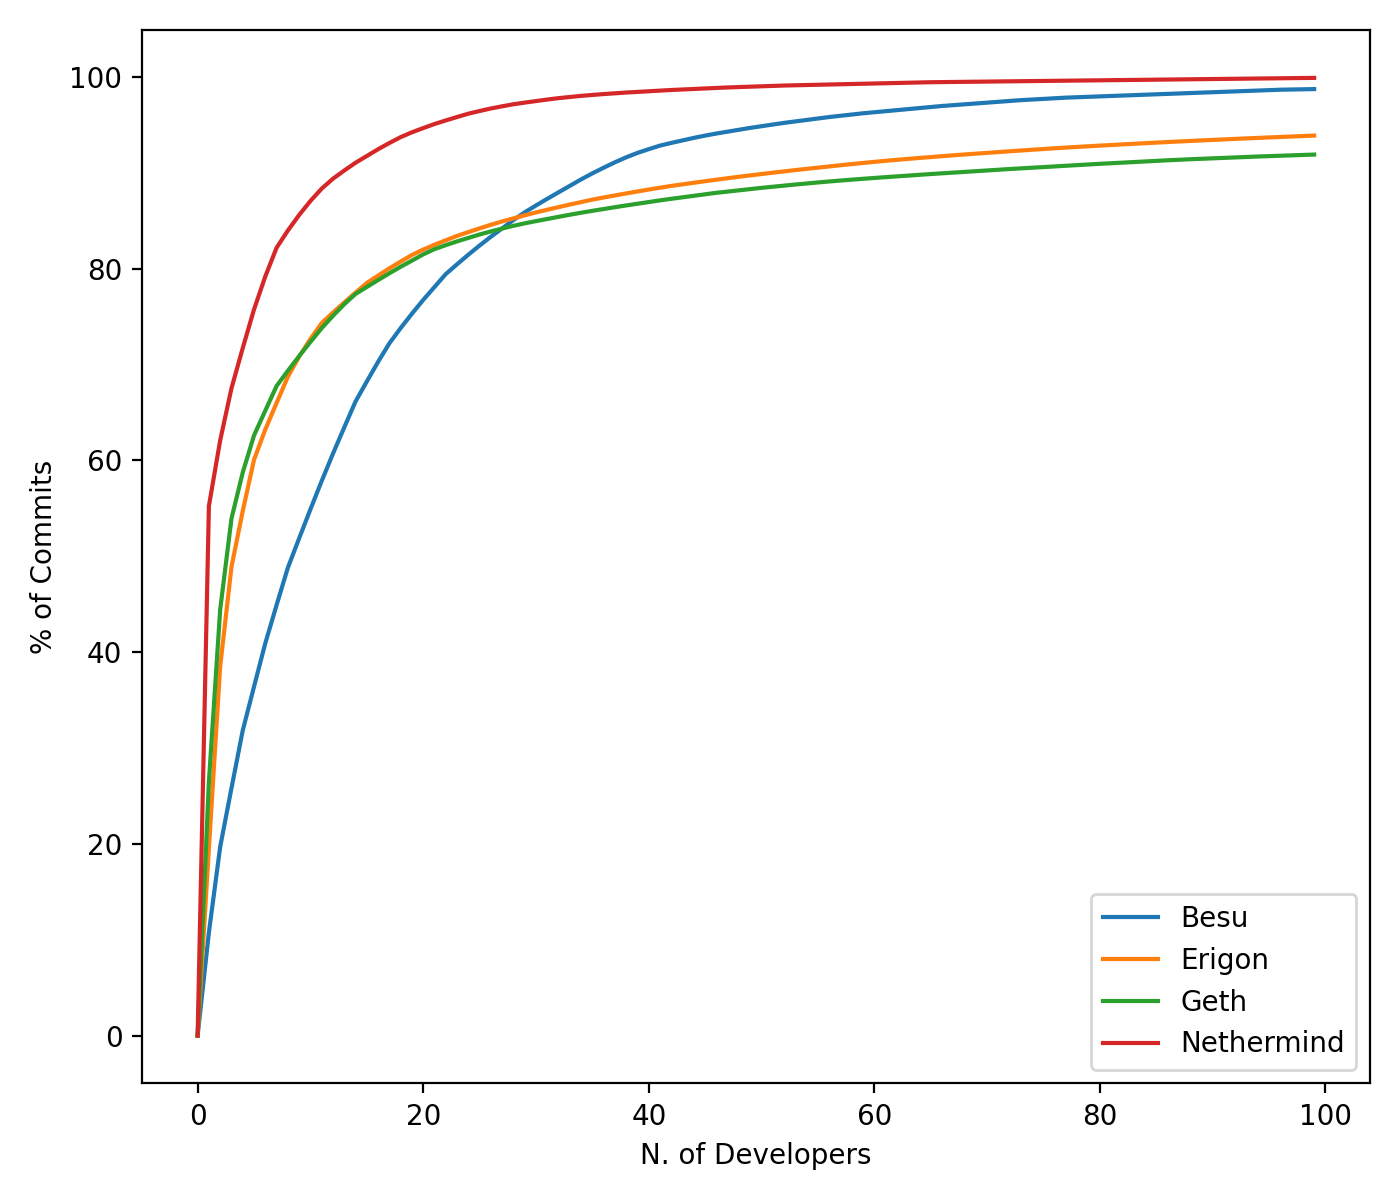
\includegraphics[width = 0.8\textwidth]{Figures/lorenz_commits.png}
    \label{fig:lorenz_commits}
\end{figure}



%%%%%%%%%%%%%%%%%%%%%%%%%%%%%%%%%%%%%%%%%%%%%%%%%%%%%%%%%%%%%%%%
\subsection{Concentration in Client Adoption} \label{subsec:concentration_Client_Adoption}
%%%%%%%%%%%%%%%%%%%%%%%%%%%%%%%%%%%%%%%%%%%%%%%%%%%%%%%%%%%%%%%%



The culmination of the EIP process is the adoption of client software updates by network nodes and participants. Figure \ref{fig:forks} shows the timeline for the most important Ethereum hard forks. Typically, these updates are ``hard forks,'' requiring nodes to upgrade by a specified deadline to maintain network compatibility. Failing to upgrade results in a network bifurcation: one with upgraded nodes and another with nodes on the older software version. This bifurcation extends to governance as well.

%%%%%%%%%%%%%%%%%%%%%%%%%%%%%%%%%%%%%%%%%%%%%%%%%%%%%%%%%%%%%%%%
\begin{figure}[ht!]
 \caption{History of Forks}
  \begin{small}
    \begin{minipage}{\textwidth}
      This figure shows the timeline of the major Ethereum hard forks. 
  \end{minipage}
    \end{small}
\makebox[\textwidth][c]{
\begin{chronology}[1]{2015}{2023}{1.1\textwidth}
\event{\decimaldate{14}{3}{2016}}{Homestead}
\event{\decimaldate{15}{7}{2016}}{DAO}
\event{\decimaldate{16}{10}{2017}}{Byzantium}
\event{\decimaldate{28}{2}{2019}}{Constantinople}
\event{\decimaldate{8}{12}{2019}}{Istanbul}
\event{\decimaldate{15}{4}{2021}}{Berlin}
\event{\decimaldate{5}{8}{2021}}{London}
\event{\decimaldate{24}{8}{2022}}{Bellatrix/Paris}
\event{\decimaldate{12}{4}{2023}}{Shapella}

\end{chronology}    \label{fig:forks}
}
\end{figure}

A prime example of this was the fork on July 20, 2016, following a vulnerability in ``The DAO'' smart contract, which led to the theft of approximately 5\% of all Ether tokens then in existence. The community's response, a contentious implementation of EIP 779, reversed Ethereum's history to a pre-attack state. Not all participants agreed, leading to a split into two distinct blockchain networks and tokens: Ethereum and Ethereum Classic. This divergence marked not just a split in transaction histories but also in governance, contributors, and client developers.

Another notable, albeit minor, disagreement occurred in 2022 during Ethereum's shift from proof-of-work to proof-of-stake. A faction of miners and participants, resistant to this change, opted not to upgrade, leading to another split. However, most software updates have been universally accepted without causing network or governance forks.

As the Ethereum ecosystem has grown since the 2016 DAO fork, any major network division now risks a greater loss of network externalities. Consequently, the likelihood increases that the vast majority of participants will align with the fork receiving the most support. In this section, we explore two centralization vectors in the adoption of new client updates: stablecoin issuers and oracle providers.

%%%%%%%%%%%%%%%%%%%%%%%%%%%%%%%%%%%%%%%%%%%%%%%%%%%%%%%%%%%%%%%%
%\subsubsection{Stablecoin Issuers and Their Influence on EIP Adoption}
%%%%%%%%%%%%%%%%%%%%%%%%%%%%%%%%%%%%%%%%%%%%%%%%%%%%%%%%%%%%%%%%

Stablecoin issuers face a unique challenge in the event of a network fork: they must choose a single chain, as their stablecoins are backed one-to-one by off-chain reserves, usually consisting of cash and cash equivalents. The stablecoins on the supported chain instance will still be redeemable and priced accordingly, while the ``stablecoins'' on the chain instance that is not supported by the issuer would be worthless. Considering the fact that stablecoins are being used as collateral across a large variety of smart contract-based financial protocols, the invalidation of a stablecoin on one blockchain instance could create systemic shocks and render many protocols on that chain dysfunctional. 

Consequently, the direction chosen by these issuers could influence the broader community's alignment. Many protocols, and by extension protocol users, are forced to follow whatever decision the stablecoin issuer might take. If the stablecoin issuer decides (not) to support an update, many protocols and financial service providers would find themselves in a difficult position, where it would be hard to oppose this decision. A high concentration in stablecoin issuance could hence grant a few entities the ability to veto or push through governance changes.

Our analysis focuses on the three predominant stablecoins on the Ethereum network: USDC, USDT, and DAI. In decentralized finance (DeFi) applications, liquidity providers lock tokens in smart contracts to facilitate token swaps or lending. We collected the Total Value Locked (TVL) for all the major liquidity pools, and flagged the ones which include one or more of the three stablecoins. Figure \ref{fig:stable_perc} shows the importance of stablecoins over time for DeFi liquidity pools. The percentage of TVL associated with stablecoins increased dramatically in early 2022, from around 15\% to 55\% of aggregate TVL in Ethereum, and then stabilized since then. As of Q3 of 2023, the stablecoin-related pools accounted for \$12.9B, or 51\% of the value of all liquidity pools. The graph shows how important stablecoins are for the Ethereum ecosystem, and thus the possible influence they might have in controversial governance discussions. 

Further, we analyze the market share of each major stablecoin. Figure \ref{fig:stable} shows that USDC has a large and growing market share of the DeFi stablecoin market. This is in contrast to the off-chain stablecoin market, where USDT is mostly used. Stablecoin issuers with large TVL market shares could become central figures in governance decisions. While their involvement in Ethereum's governance has been limited to date, the potential for their future influence, particularly on controversial EIPs concerning stablecoins, should not be underestimated.


%%%%%%%%%%%%%%%%%%%%%%%%%%%%%%%%%%%%%%%%%%%%%%%%%%%%%%%
\begin{figure}[ht!]
    \caption{Stablecoin Concentration}
     \begin{small}
    \begin{minipage}{\textwidth}
      Panel (a) shows the percentage of Total Value Locked (TVL) in liquidity pools that include one of the three major stablecoins USDC, USDT, and DAI over time. Panel (b) shows the TVL market share for each of the three major stablecoins USDC, USDT, and DAI over time.  
     \end{minipage}
         \end{small}
         \\[0.5cm]
   \begin{subfigure}{0.49\textwidth}
           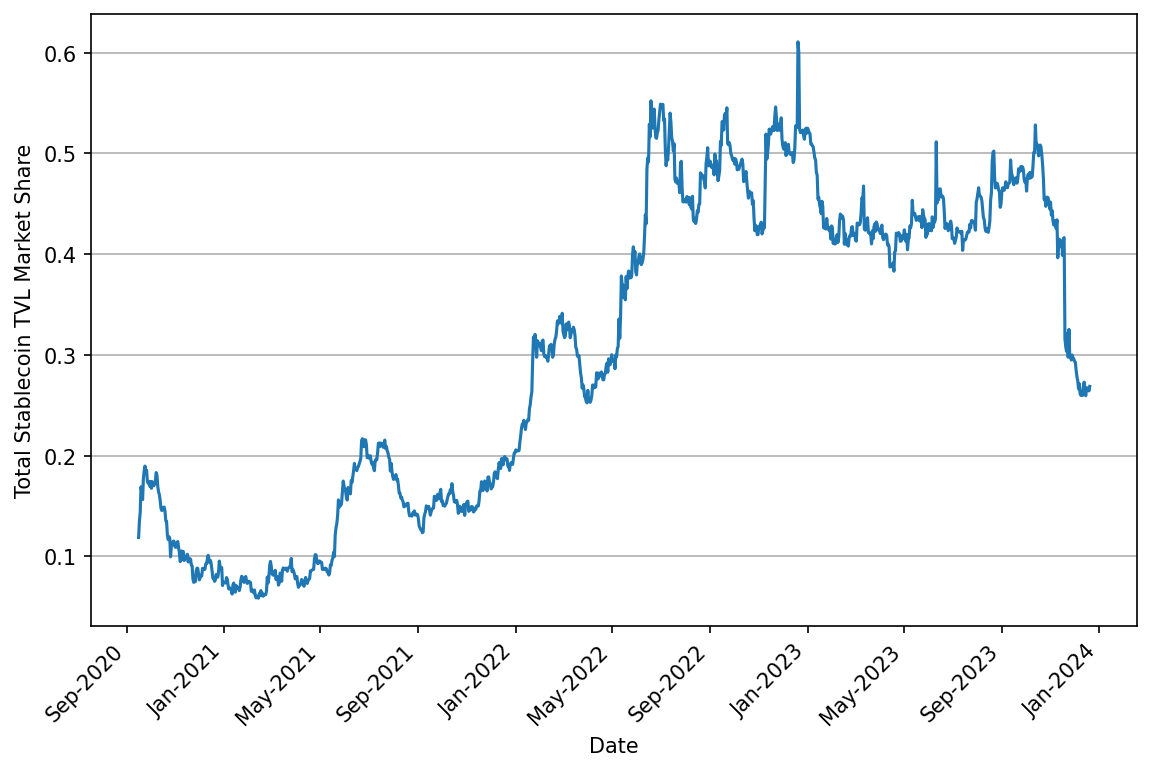
\includegraphics[width = 1\textwidth]{Figures/stable_perc.png}
            \caption{Stablecoin Percentage in All Liquidity Pools}
            \label{fig:stable_perc}
   \end{subfigure}
    \begin{subfigure}{0.49\textwidth}
           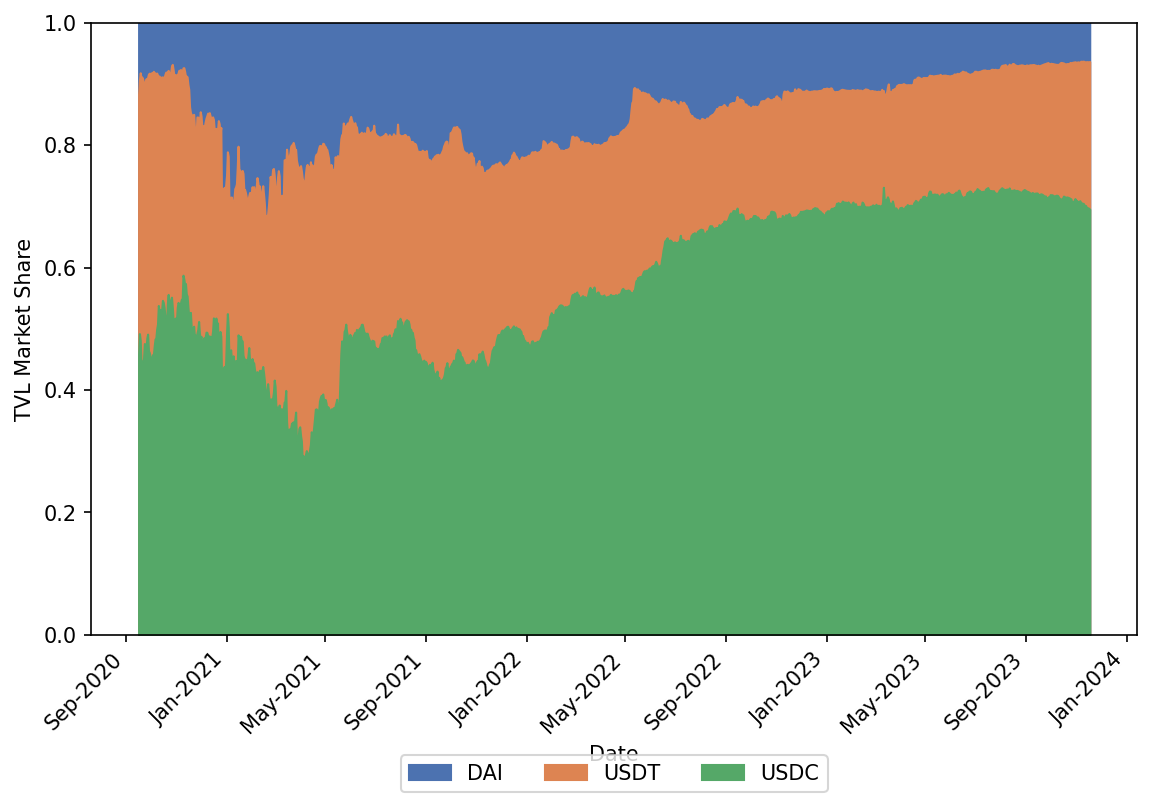
\includegraphics[width = 1\textwidth]{Figures/stable.png}
            \caption{Market Share of Major Stablecoin Issuers}
            \label{fig:stable}
   \end{subfigure}
  
\end{figure}



%%%%%%%%%%%%%%%%%%%%%%%%%%%%%%%%%%%%%%%%%%%%%%%%%%%%%%%%%%%%%%%%
%\subsubsection{The Role of Oracle Providers in EIP Adoption}
%%%%%%%%%%%%%%%%%%%%%%%%%%%%%%%%%%%%%%%%%%%%%%%%%%%%%%%%%%%%%%%%

Oracles represent another potential governance concentration vector. Many smart contracts depend on external data, sourced from oracles, for critical functions like maintaining collateralization ratios in borrowing and lending platforms. A dominant oracle provider's refusal to support a network upgrade could severely disrupt numerous DeFi applications. In turn, this means that oracles with large market shares could influence the governance process with their effective veto power. We identify the largest DeFi protocols that use oracle providers, and collect the total value locked (TVL) in these protocols using data from DefiLlama.com. Overall, over 200 protocols use oracle providers to receive on-chain and off-chain data for their smart contracts, with an aggregate TVL of \$23.5B. Panel (a) of Figure \ref{fig:oracle} shows the market share of oracles by protocol TVL. Similar to  \cite{cong2023financial}, we find that Chainlink and Chronicle provide oracle services to protocols that account for 90\% of the TVL. However, Chronicle is primarily used only by one large protocol, MakerDAO. In fact, panel (b) shows that Chainlink is the oracle used by the vast majority of protocols. The extensive reliance on Chainlink by most DeFi applications raises concerns. This reliance not only poses risks regarding the potential exploitation of smart contracts but also represents another facet of governance centralization and reverse dependency within the Ethereum ecosystem.


%%%%%%%%%%%%%%%%%%%%%%%%%%%%%%%%%%%%%%%%%%%%%%%%%%%%%%%
\begin{figure}[ht!]
    \caption{Oracle Concentration}
     \begin{small}
    \begin{minipage}{\textwidth}
      Panel (a) shows the percentage of Total Value Locked (TVL) in liquidity pools that use a specific oracle provider. Panel (b) shows the number of protocols that use a specific oracle provider. Data from DefiLlama.com
     \end{minipage}
         \end{small}
         \\[0.5cm]
   \begin{subfigure}{0.49\textwidth}
           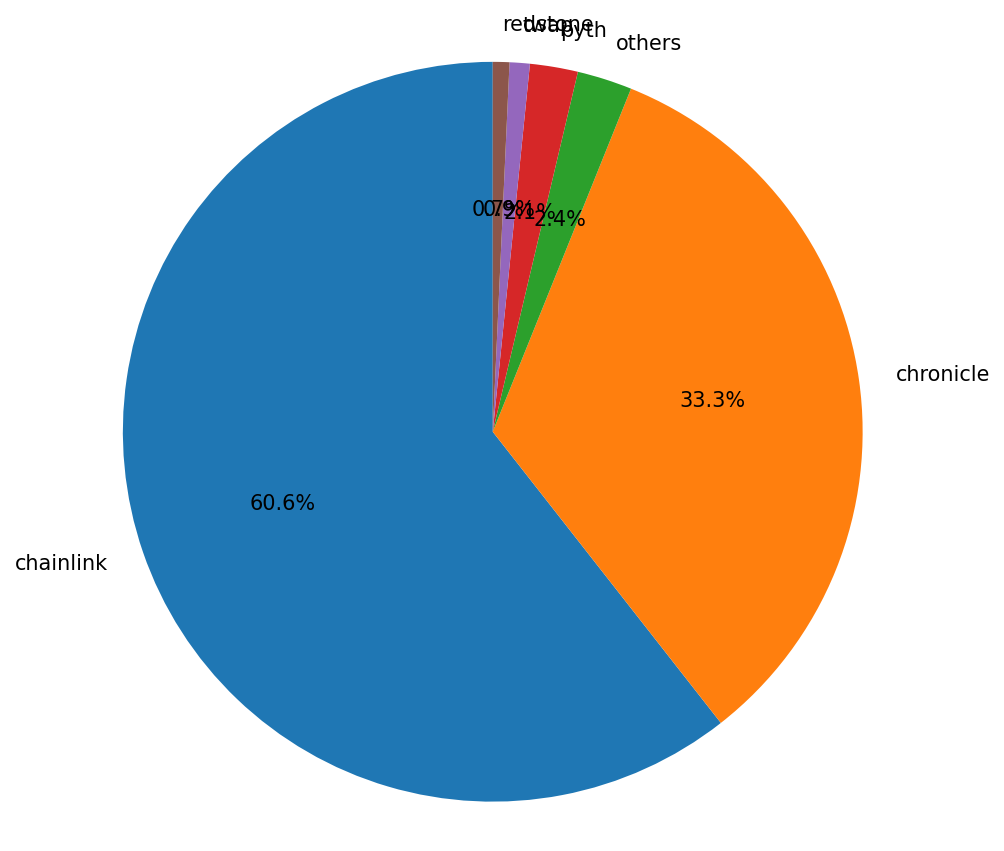
\includegraphics[width = 1\textwidth]{Figures/oracle_pie.png}
            \caption{Protocols TVL by Oracle}
            \label{fig:oracle_pie}
   \end{subfigure}
    \begin{subfigure}{0.49\textwidth}
           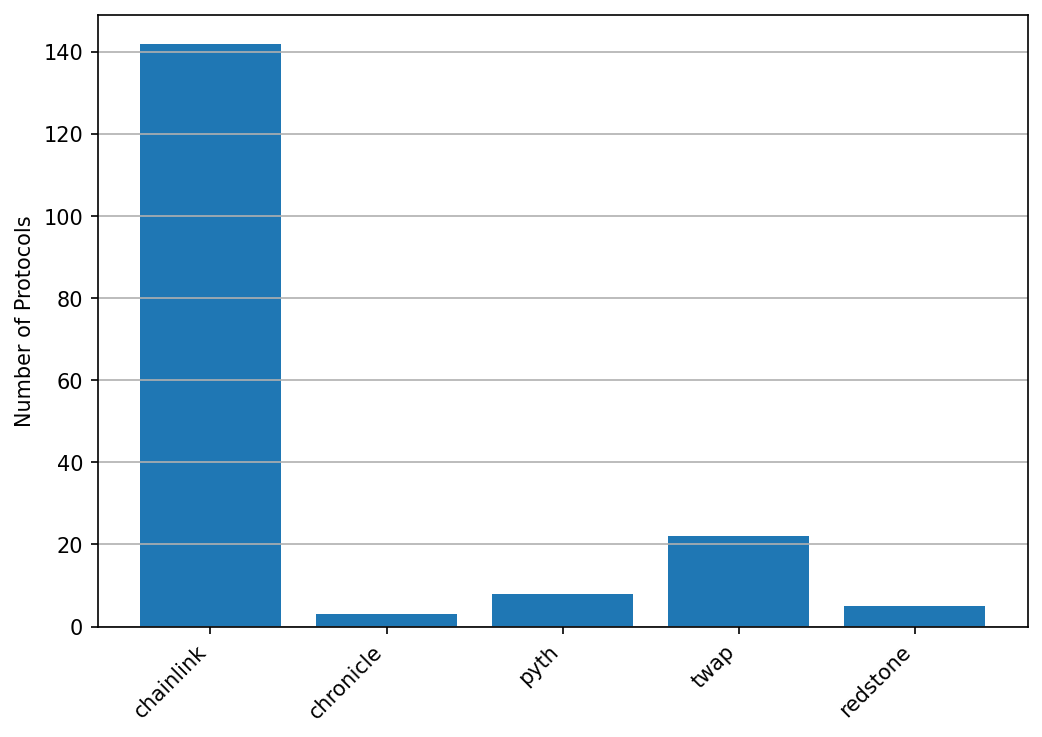
\includegraphics[width = 1\textwidth]{Figures/oracle_bar.png}
            \caption{Number of Protocols by Oracle}
            \label{fig:oracle_bar}
   \end{subfigure}
  \label{fig:oracle}
\end{figure}





%%%%%%%%%%%%%%%%%%%%%%%%%%%%%%%%%%%%%%%%%%%%%%%%%%%%%%%%%%%%%%%%
%%%%%%%%%%%%%%%%%%%%%%%%%%%%%%%%%%%%%%%%%%%%%%%%%%%%%%%%%%%%%%%%
\subsection{The Influence of the Ethereum Foundation and other Entities} \label{subsec:companies}
%%%%%%%%%%%%%%%%%%%%%%%%%%%%%%%%%%%%%%%%%%%%%%%%%%%%%%%%%%%%%%%%
%%%%%%%%%%%%%%%%%%%%%%%%%%%%%%%%%%%%%%%%%%%%%%%%%%%%%%%%%%%%%%%%

The involvement of developers in Ethereum governance is a voluntary effort, often balanced alongside their full-time employment. This raises a pertinent question about the alignment of authors' incentives with the objectives of their employers. Historically, open-source communities have held mixed perspectives on the involvement of for-profit companies in open source project development and support. On one hand, these companies contribute valuable financial and human resources to open source initiatives, which are often resource-constrained. Conversely, concerns have arisen regarding the potential for undue influence exerted by companies on the trajectory of open source projects. The literature on open source identifies trust as central to sustained contributor participation (see \cite{Jarvenpaaetal2004}, \cite{Korsgaardetal1995}, and \cite{StewartGosain2006}). Continued participation therefore depends on governance that contributors see as fair, where their voices are heard and all participants work towards the project's greater good, rather than governance dominated by the for-profit interests of a single company or a group of companies.

To explore the impact of company affiliations, we examined the current employment status of all EIP authors and client developers. We gathered details about their current and previous jobs from LinkedIn and linked these with their contributions to various EIPs and Ethereum clients. Most of these contributors, actively engaged in EIPs, are volunteers with full-time roles in firms, often linked to the cryptocurrency sector. Our findings, illustrated in Figure \ref{fig:ncomp}, cover the employment affiliations of EIP authors in panels (a) to (c) and client developers in panel (d).

Our methodology for assessing the influence of these companies on EIP introductions involved tallying unique authors and their company affiliations. However, this approach does not account for the possibility that prolific authors may be associated with specific companies. Therefore, we also tracked the number of EIPs co-authored by individuals linked to each company.

First, the data reveals that the Ethereum community exhibits a remarkably diverse range of employment backgrounds, with no single company representing more than 3.5\% of all authors. The blue line in panel (a) of figure \ref{fig:ncomp} is very close to the 45-degree line, demonstrating a fairly even distribution of company participation in Ethereum governance, as indicated by a Gini coefficient of 0.15. Panel (b) reveals that the Ethereum Foundation, followed by Consensys and Coinbase, employs the largest number of authors. However, this does not fully capture the influence of companies, because prolific authors could cluster in specific companies. Panel (a)'s red line indicates a moderate concentration of EIPs authored by individuals from specific companies, with a Gini coefficient of 0.50. Panel (c) shows that over 20\% of all EIPs were co-authored by individuals employed by the Ethereum Foundation. 

Shifting focus to client development, we identified the main employers of the top 20 developers for each client, who collectively are responsible for over 80\% of all commits. Our findings, as shown in panel (d), reveal that each client benefits from the backing of a prominent organization: the Ethereum Foundation supports all four main clients included in our analysis: Erigon, Geth, Besu, and Nethermind. Some clients receive additional funding from firms like Consensys, public grants or have additional business models like auditing services.\footnote{See e.g., \url{https://blog.ethereum.org/2021/03/23/supporting-ethereums-client-ecosystem} or \url{https://blog.ethereum.org/2021/08/24/building-together}}

%%%%%%%%%%%%%%%%%%%%%%%%%%%%%%%%%%%%%%%%%%%%%%%%%%%%%%%
\begin{figure}[ht!]
    \caption{Organizations Affiliated with EIP Authors and Client Developers}
     \begin{small}
    \begin{minipage}{\textwidth}
      Panel (a) shows the Lorenz curve for affiliated company concentration in EIPs and authors. Panel (b) counts how many authors are employed by an affiliated company. Panel (c) counts the number of EIPs co-authored by at least one individual who is affiliated with a company. Panel (d) shows the percentage of top-20 client developers working for affiliated companies for each of the four main clients.  
  \end{minipage}
     \end{small}
         \\[0.5cm]
  \begin{subfigure}{0.49\textwidth}
           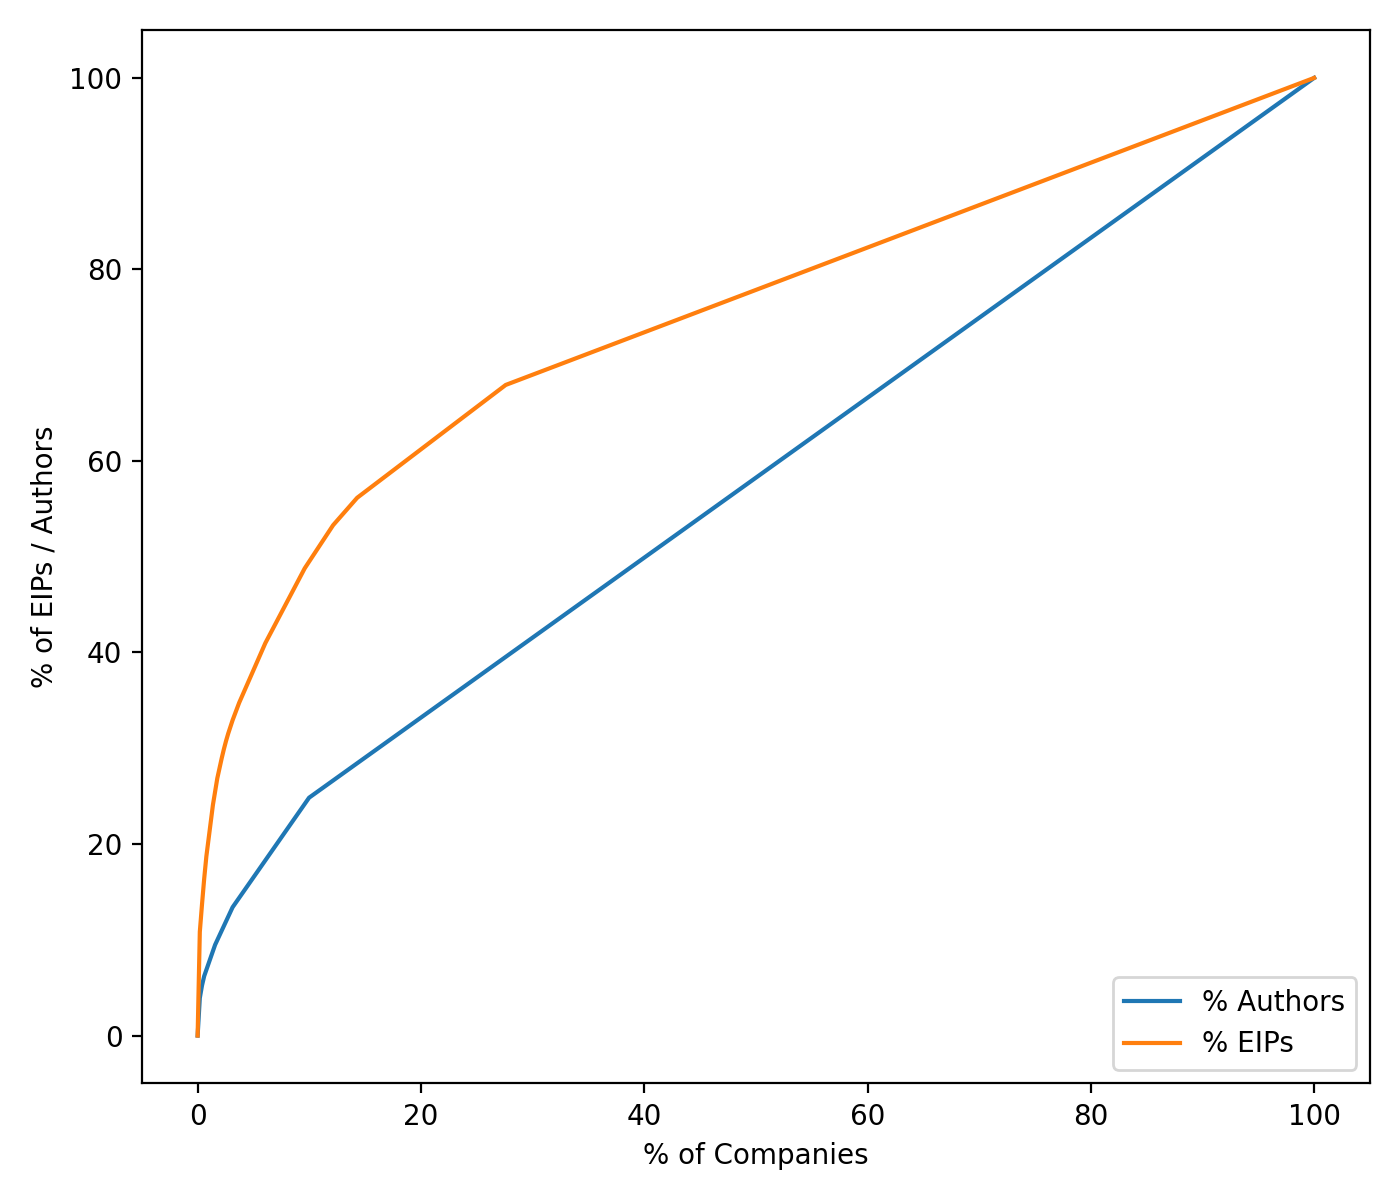
\includegraphics[width = 1\textwidth]{Figures/company_lorenz.png}
            \caption{by EIP}
            \label{fig:ncomp_lorenz}
   \end{subfigure}
   \begin{subfigure}{0.49\textwidth}
           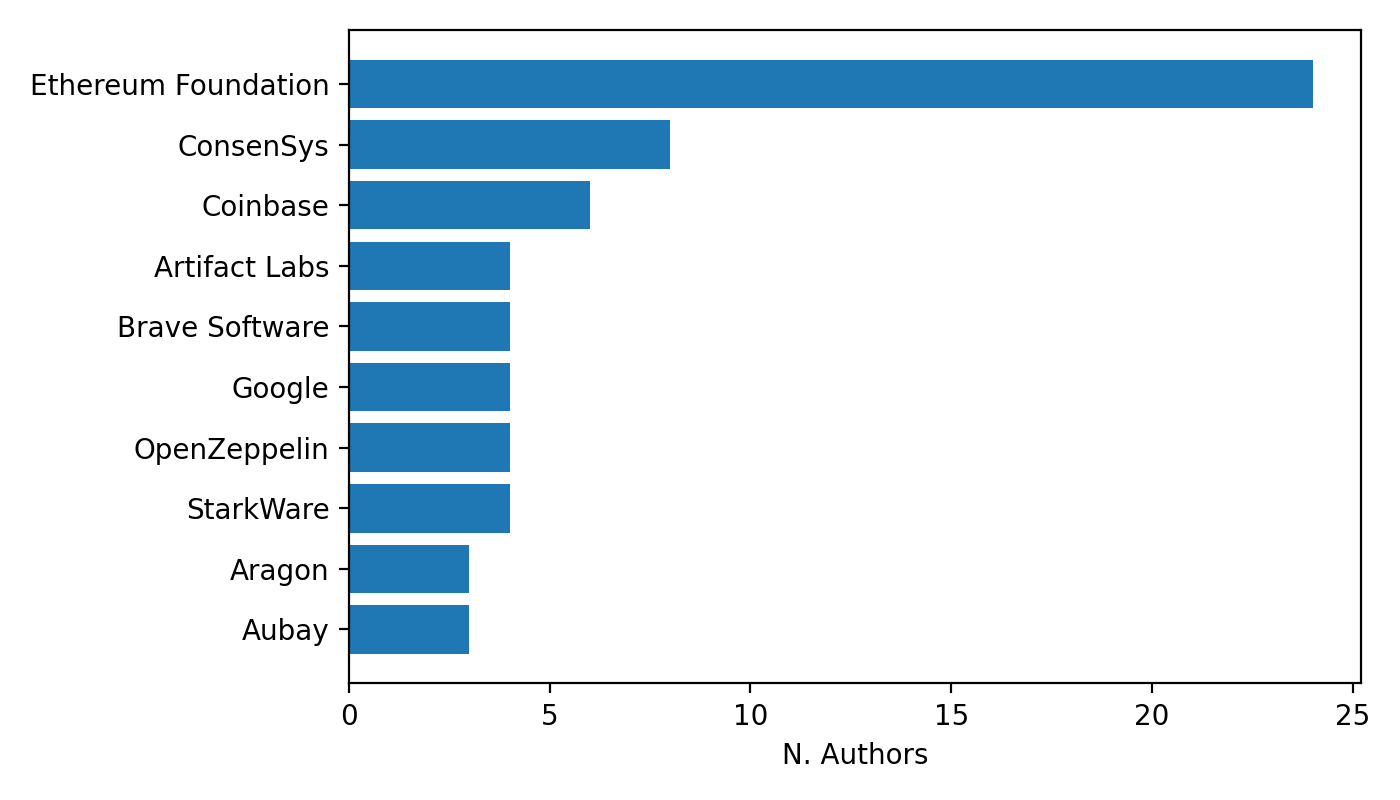
\includegraphics[width = 1\textwidth]{Figures/company_neip2.png}
            \caption{by Author}
            \label{fig:ncomp_author}
   \end{subfigure}
       \\[0.5cm]
   \begin{subfigure}{0.49\textwidth}
           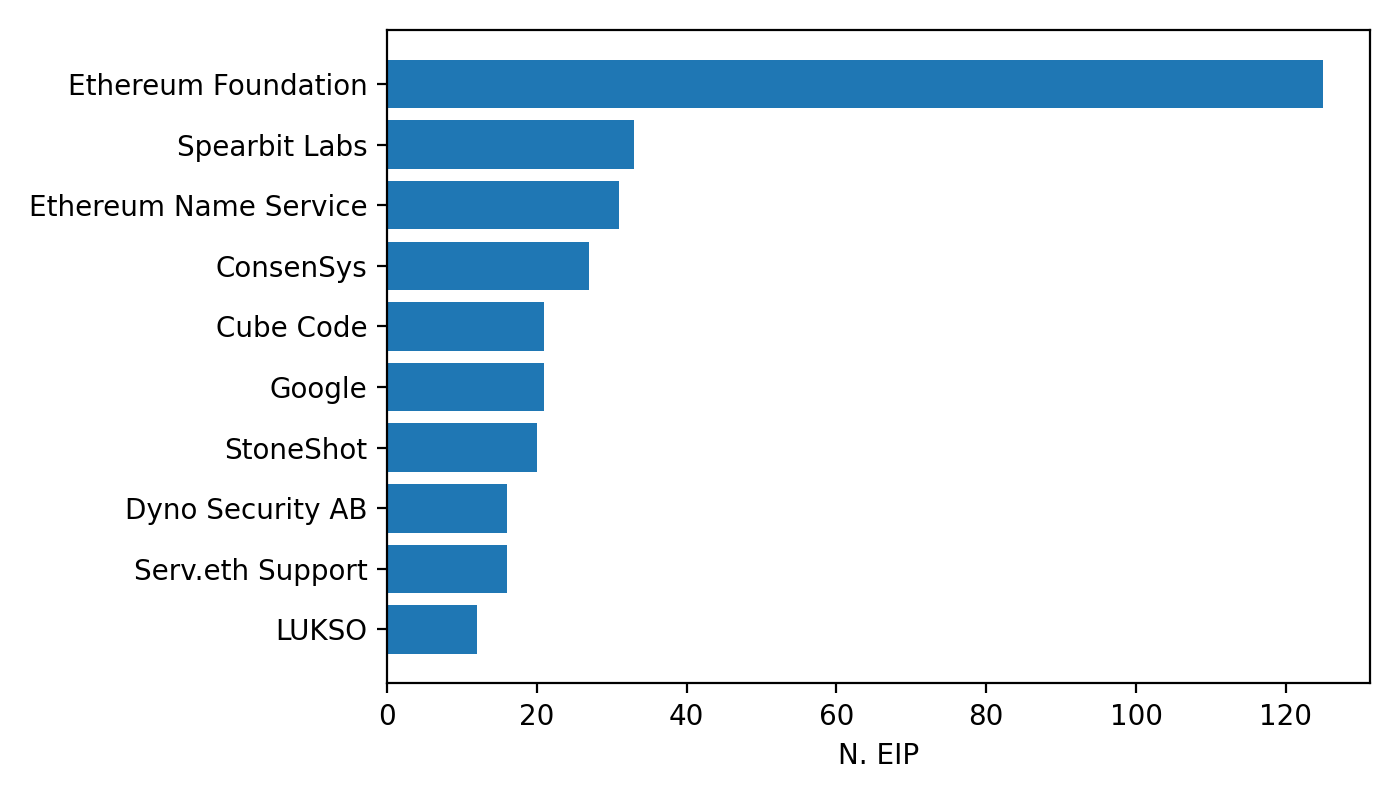
\includegraphics[width = 1\textwidth]{Figures/company_neip3.png}
            \caption{by EIP}
            \label{fig:ncomp_eipauthor}
   \end{subfigure}
  \begin{subfigure}{0.49\textwidth}
           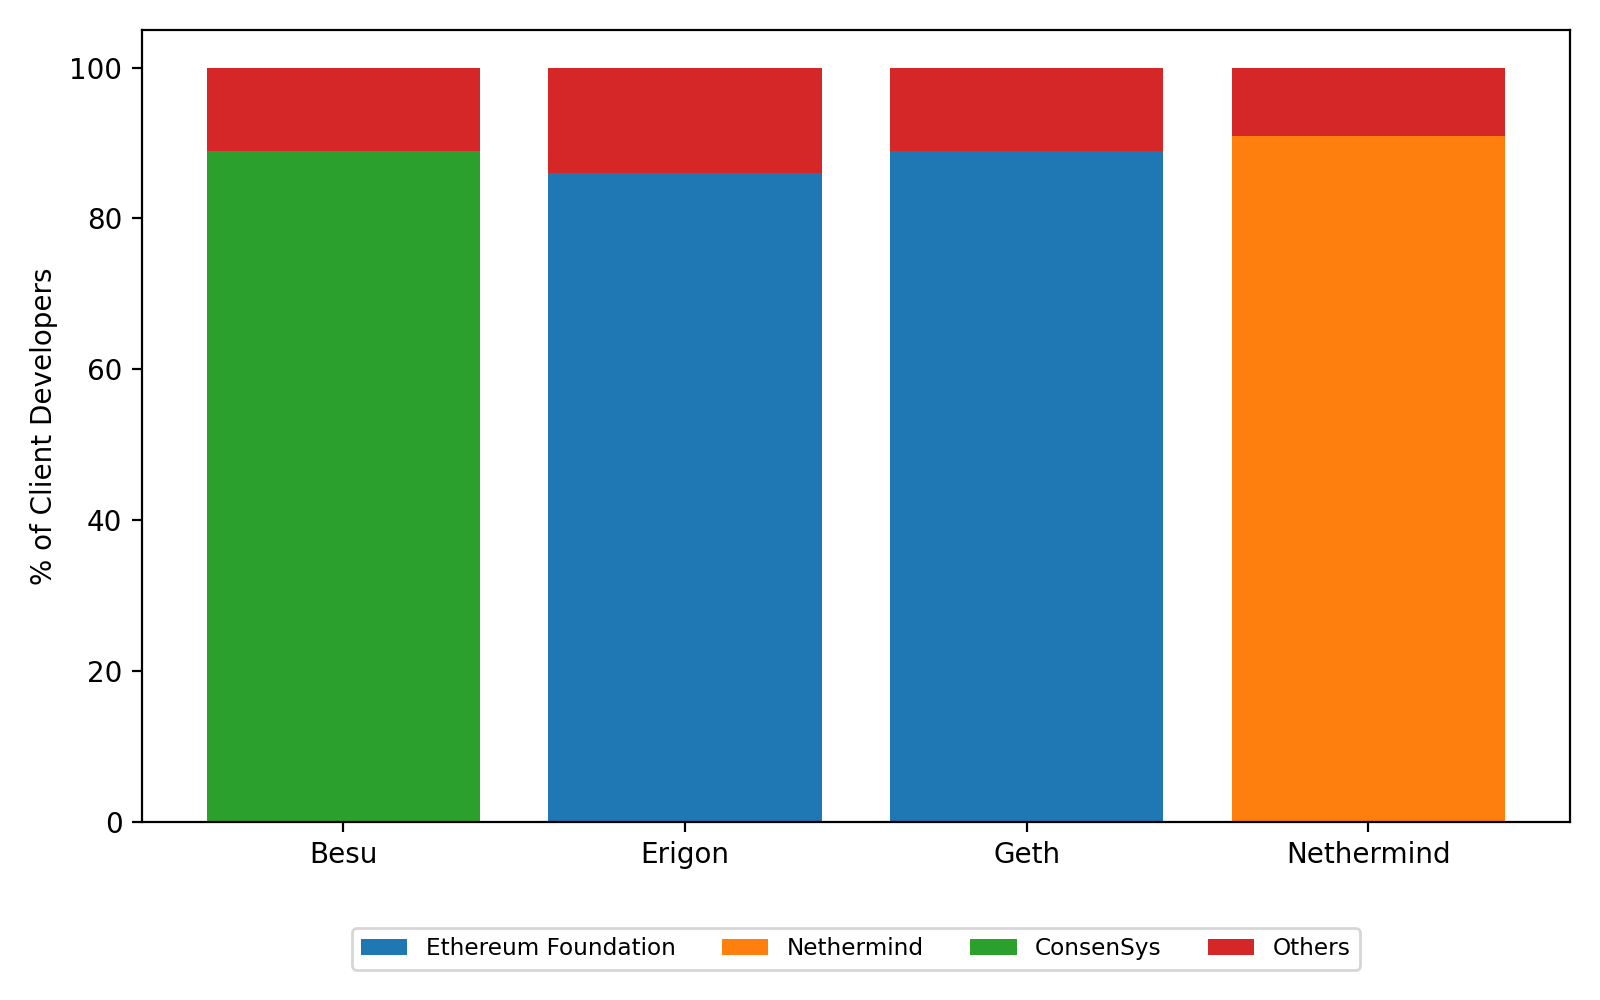
\includegraphics[width = 1\textwidth]{Figures/client_company.png}
            \caption{by Client}
            \label{fig:client_company}
   \end{subfigure}
   \label{fig:ncomp}
\end{figure}

Overall, the Ethereum Foundation's influence in both EIP production and client development has persisted throughout our study period, as shown in figure \ref{fig:ef_year}. As discussed in section \ref{sec:transparency}, the Ethereum Foundation was instrumental in the initial development stages of the Ethereum protocol. This leads us to question whether the Foundation's influence has waned over time. Figure \ref{fig:ef_year} plots the annual proportion of EIPs co-authored by someone from the Ethereum Foundation. Initially, the Foundation was involved in about 75\% of all EIPs, but this figure has declined sharply to under 20\% in recent years. However, the decline seems to be mostly due to ERC EIPs, in the red line. The percentage of core EIPs with some involvement of the Ethereum Foundation has been slowly increasing since 2019, reaching over 40\% of core EIPs today. The divergence in the Ethereum Foundation's involvement between core and ERC EIPs aligns with the initial steps towards the transition from Proof-of-Work to Proof-of-Stake and may be related to increased specialization and complexity of the proposals.

%%%%%%%%%%%%%%%%%%%%%%%%%%%%%%%%%%%%%%%%%%%%%%%%%%%%%%%
\begin{figure}[ht!]
    \caption{Influence of Ethereum Foundation over Time}
     \begin{small}
    \begin{minipage}{\textwidth}
      This figure shows the percentage of EIPs produced for each two-year rolling window where at least one author is affiliated with the Ethereum Foundation over time. Year 2023 numbers are incomplete, as data collection ended on June 21, and are marked with an asterisk.
  \end{minipage}
         \end{small}
    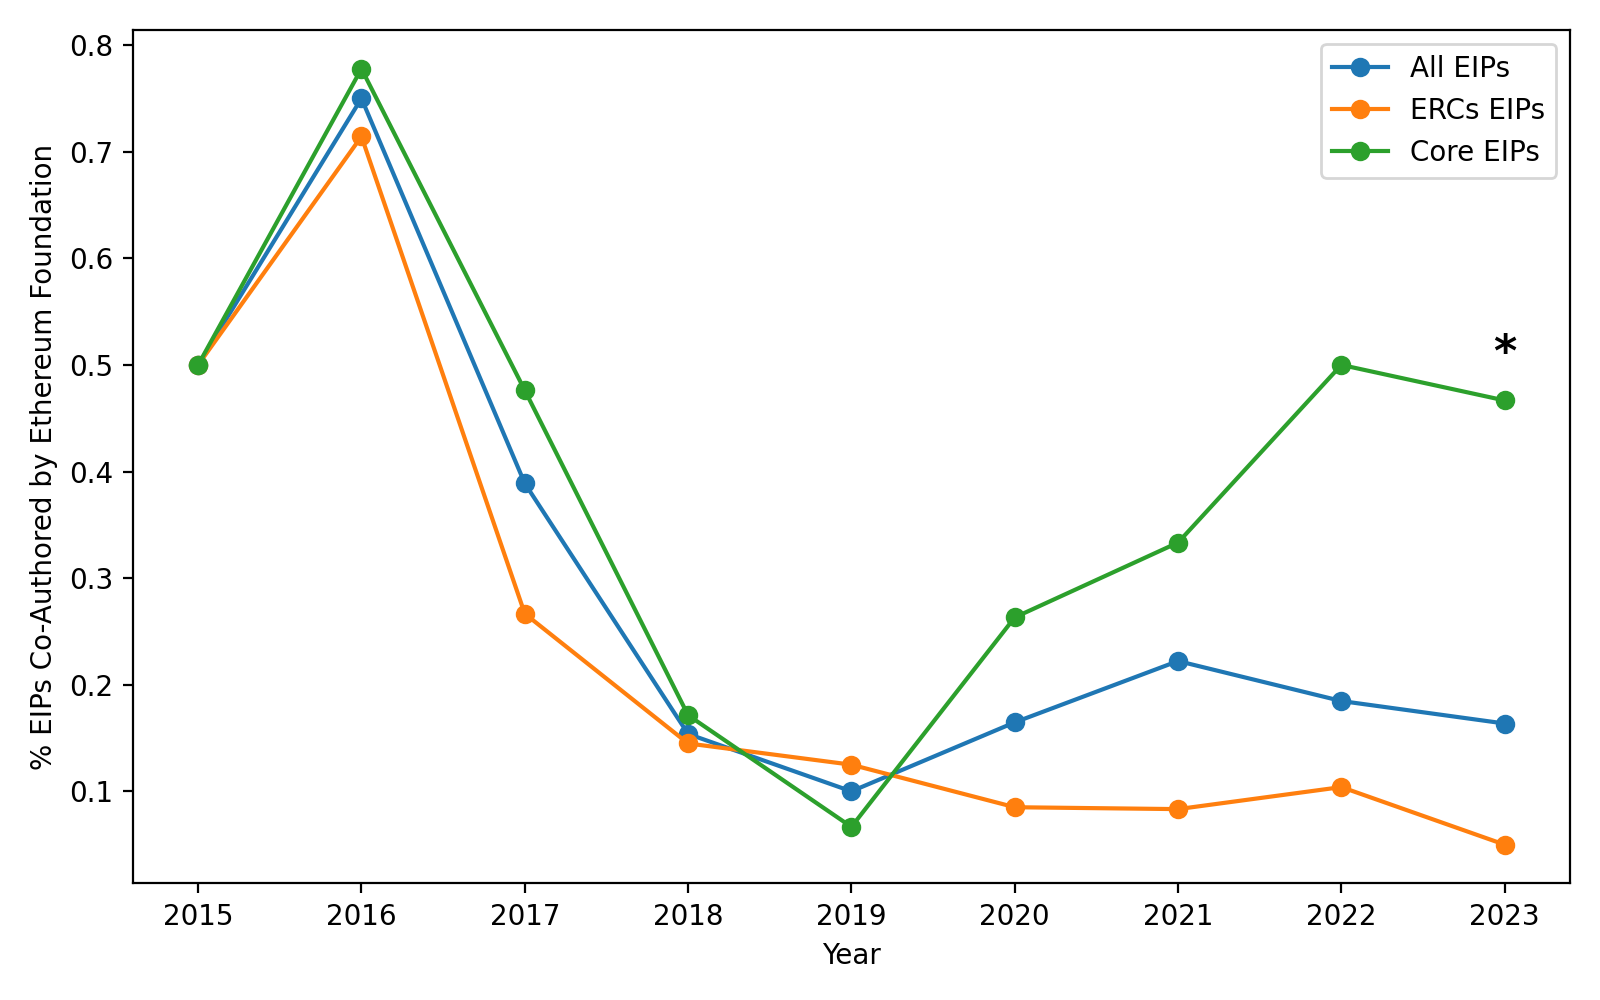
\includegraphics[width = 0.8\textwidth]{Figures/eip_ef_by_year.png}\label{fig:ef_year}
\end{figure}
%%%%%%%%%%%%%%%%%%%%%%%%%%%%%%%%%%%%%%%%%%%%%%%%%%%%%%%

%%%%%%%%%%%%%%%%%%%%%%%%%%%%%%%%%%%%%%%%%%%%%%%%%%%%%%%
%%%%%%%%%%%%%%%%%%%%%%%%%%%%%%%%%%%%%%%%%%%%%%%%%%%%%%%


Taken together, the evidence indicates that Ethereum governance is characterized by broad participation but substantial concentration at the stages that are most consequential for the protocol's development. While hundreds of individuals participate in EIP production and discussion, the proposals that ultimately affect the core protocol are disproportionately associated with a relatively small group of authors, developers, and organizations. This concentration becomes particularly pronounced during client implementation, where a small number of developers account for the majority of commits, and can extend to client adoption through the influence of economically important intermediaries such as stablecoin issuers and oracle providers. The resulting governance structure therefore differs from a model in which decision-making authority is broadly dispersed: influence is distributed across multiple actors, but meaningful control can become concentrated at successive points along the path from proposal to implementation and adoption. This structure is relevant to the three corporate governance concerns examined in this paper. First, concentrated participation may create opportunities for insider information, as individuals involved in multiple stages of the process may learn about material protocol changes before they become widely understood by the broader market. Second, concentration raises questions of liability, since identifying the individuals or entities responsible for a consequential governance decision becomes more difficult when authority is informal, distributed across organizations, and not tied to a conventional corporate hierarchy. Third, overlapping affiliations and the economic importance of particular companies, developers, and infrastructure providers create potential conflicts of interest, particularly when participants may simultaneously contribute to Ethereum's development and have commercial interests affected by particular protocol changes. Thus, the relevant issue is not simply whether Ethereum governance is decentralized in aggregate, but whether decision-making power, information, and incentives remain sufficiently dispersed at the specific stages where consequential governance decisions are made.



%%%%%%%%%%%%%%%%%%%%%%%%%%%%%%%%%%%%%%%%%%%%%%%%%%%%%%%
%%%%%%%%%%%%%%%%%%%%%%%%%%%%%%%%%%%%%%%%%%%%%%%%%%%%%%%
%%%%%%%%%%%%%%%%%%%%%%%%%%%%%%%%%%%%%%%%%%%%%%%%%%%%%%%

%%%%%%%%%%%%%%%%%%%%%%%%%%%%%%%%%%%%%%%%%%%%%%%%%%%%%%%
%%%%%%%%%%%%%%%%%%%%%%%%%%%%%%%%%%%%%%%%%%%%%%%%%%%%%%%
%%%%%%%%%%%%%%%%%%%%%%%%%%%%%%%%%%%%%%%%%%%%%%%%%%%%%%%

\section{Conclusion}

Our analysis of Ethereum's governance process examines three classical corporate governance concerns in the context of an open-source community: (i) the availability and importance of information, (ii) the alignment of contributors' incentives, and (iii) the concentration of effective control.

Our analysis suggests that most of the relevant information about Ethereum's governance is publicly available, and anyone is able to contribute to the governance process. We were able to obtain the history of governance proposals, collect data from discussion forums and developer meetings, and follow proposals through implementation in client software and adoption by the network. This high level of openness distinguishes Ethereum governance from traditional organizational structures. At the same time, the public availability of information does not imply that it is equally accessible or easy to interpret. The technical complexity of proposals, the distributed nature of the governance process, and the volume of available information can make it difficult for outside participants to understand the implications of a proposed change. The information is therefore public, but not necessarily costless to process.

This distinction matters for the first governance concern: the potential for information asymmetries. The Ethereum governance process provides extensive visibility into proposals, discussions, developer calls, and implementation. Most participants also disclose their identities, making the individuals involved in consequential decisions identifiable. Yet the technical nature of the process means that meaningful information may remain concentrated among participants with the expertise to evaluate particular proposals. The absence of a formal organizational hierarchy also means that there is no clearly defined management group with conventional disclosure obligations. Thus, transparency substantially limits the scope for purely private information, while specialized knowledge and the complexity of the governance process can still create differences in who is able to interpret publicly available information.

Our analysis of the effect of governance on token value shows that governance milestones contain economically relevant information. In particular, EIP finalization is associated with changes in the price of Ether, indicating that the market responds to information about the resolution of governance proposals. This finding is important for the broader governance analysis because it establishes that protocol governance is not merely a technical process: decisions made through the governance process can have direct financial consequences for token holders.

The price response also creates a potential information advantage for participants who are closely involved in the development and finalization of protocol changes. In this setting, the openness of the governance process may limit information asymmetries, but it does not eliminate them, since participants with specialized knowledge or early access to information may be better positioned to interpret or anticipate governance outcomes. More broadly, the fact that governance milestones are reflected in token prices connects the governance process to the incentives of contributors and to the potential conflicts that can arise when individuals involved in protocol development also have economic exposure to the token.

The second part of our analysis concerns the incentives of contributors. Unlike a traditional firm, Ethereum does not employ the individuals responsible for proposing and implementing protocol changes, and there is no contractual relationship through which the protocol can directly compensate contributors. Our evidence indicates that labor-market returns provide an important alternative incentive mechanism. Following the introduction of an EIP, authors experience increases in employment seniority and estimated compensation, with the effects particularly pronounced among junior contributors. These results are consistent with the signaling mechanism emphasized in the open-source literature: participation in Ethereum governance provides contributors with a visible opportunity to demonstrate technical ability and receive subsequent labor-market rewards. Taken together, these mechanisms suggest that contributors can have meaningful economic incentives to participate in maintaining and improving Ethereum even in the absence of a conventional employment relationship.

The third part of our analysis concerns effective control. The data indicate that broad participation in discussion does not translate into equally broad participation at every stage of the governance process. Hundreds of individuals contribute to EIP production and discussion, and the authorship network has become more interconnected over time. However, when we focus on proposals that affect the underlying protocol, the number of relevant contributors declines substantially. The ten most prolific authors account for 62\% of implemented Core and Networking EIPs, and client software development is even more concentrated, with a Gini coefficient of approximately 89\%. The concentration of implementation therefore creates an important distinction between participation in governance and effective influence over protocol changes.

The distribution of control also extends beyond individual contributors. No single company accounts for more than 3.5\% of the EIP author pool, indicating substantial diversity in the employment backgrounds of contributors. At the same time, the Ethereum Foundation has been involved in more than 20\% of EIPs and continues to have a substantial presence in core protocol development. This concentration does not necessarily imply that the Foundation controls Ethereum's governance. Rather, it illustrates how influence can arise through sustained participation in the development and implementation of protocol changes even when formal authority is absent. The same distinction applies to client development, where a small number of developers account for a large share of contributions despite a much larger pool of individuals making occasional contributions.

Finally, effective control can arise at the adoption stage through actors that are not formally part of Ethereum's governance process. Stablecoin issuers and oracle providers are important examples. Because many applications depend on these services, their decisions about which version of the network to support can influence whether a protocol upgrade is ultimately adopted. These reverse dependencies introduce an additional form of concentration: an actor need not participate directly in the EIP process to acquire meaningful influence over its outcome. As Ethereum becomes an increasingly important infrastructure for financial applications, these dependencies become an important part of understanding where effective control resides.

Our analysis therefore suggests that Ethereum governance combines broad participation and substantial transparency with meaningful concentration at the stages where protocol changes are proposed, implemented, and adopted. The governance process differs fundamentally from a conventional corporation: there is no board, no formal management hierarchy, and no contractual employment relationship connecting contributors to the protocol. Yet the absence of these formal structures does not eliminate the underlying governance concerns. Information can become concentrated through technical expertise, incentives can operate through token holdings and labor-market returns, and effective control can become concentrated among particular contributors, organizations, and infrastructure providers. Read together, these findings are consistent with \cite{Olson1965}’s and \cite{Ostrom1990}’s accounts of collective action: a non-rival public good is under-provided by the group at large, but sustained by a smaller set of participants who capture a private benefit large enough to justify the cost of contributing and who, through transparency and reputational monitoring, keep the system functioning without a formal hierarchy.

Our analysis provides an initial empirical characterization of these mechanisms. Further research is needed to understand how governance concentration evolves as the protocol becomes more technically complex, how contributors' incentives interact with their affiliations and token holdings, and how dependencies on external infrastructure affect the distribution of effective control.

\newpage
\bibliographystyle{aea}
\bibliography{bib.bib}

\end{document}
